% Options for packages loaded elsewhere
% Options for packages loaded elsewhere
\PassOptionsToPackage{unicode}{hyperref}
\PassOptionsToPackage{hyphens}{url}
\PassOptionsToPackage{dvipsnames,svgnames,x11names}{xcolor}
%
\documentclass[
  spanish,
  letterpaper,
  DIV=11,
  numbers=noendperiod]{scrreprt}
\usepackage{xcolor}
\usepackage{amsmath,amssymb}
\setcounter{secnumdepth}{5}
\usepackage{iftex}
\ifPDFTeX
  \usepackage[T1]{fontenc}
  \usepackage[utf8]{inputenc}
  \usepackage{textcomp} % provide euro and other symbols
\else % if luatex or xetex
  \usepackage{unicode-math} % this also loads fontspec
  \defaultfontfeatures{Scale=MatchLowercase}
  \defaultfontfeatures[\rmfamily]{Ligatures=TeX,Scale=1}
\fi
\usepackage{lmodern}
\ifPDFTeX\else
  % xetex/luatex font selection
  \setmainfont[]{Calibri}
\fi
% Use upquote if available, for straight quotes in verbatim environments
\IfFileExists{upquote.sty}{\usepackage{upquote}}{}
\IfFileExists{microtype.sty}{% use microtype if available
  \usepackage[]{microtype}
  \UseMicrotypeSet[protrusion]{basicmath} % disable protrusion for tt fonts
}{}
\makeatletter
\@ifundefined{KOMAClassName}{% if non-KOMA class
  \IfFileExists{parskip.sty}{%
    \usepackage{parskip}
  }{% else
    \setlength{\parindent}{0pt}
    \setlength{\parskip}{6pt plus 2pt minus 1pt}}
}{% if KOMA class
  \KOMAoptions{parskip=half}}
\makeatother
% Make \paragraph and \subparagraph free-standing
\makeatletter
\ifx\paragraph\undefined\else
  \let\oldparagraph\paragraph
  \renewcommand{\paragraph}{
    \@ifstar
      \xxxParagraphStar
      \xxxParagraphNoStar
  }
  \newcommand{\xxxParagraphStar}[1]{\oldparagraph*{#1}\mbox{}}
  \newcommand{\xxxParagraphNoStar}[1]{\oldparagraph{#1}\mbox{}}
\fi
\ifx\subparagraph\undefined\else
  \let\oldsubparagraph\subparagraph
  \renewcommand{\subparagraph}{
    \@ifstar
      \xxxSubParagraphStar
      \xxxSubParagraphNoStar
  }
  \newcommand{\xxxSubParagraphStar}[1]{\oldsubparagraph*{#1}\mbox{}}
  \newcommand{\xxxSubParagraphNoStar}[1]{\oldsubparagraph{#1}\mbox{}}
\fi
\makeatother

\usepackage{color}
\usepackage{fancyvrb}
\newcommand{\VerbBar}{|}
\newcommand{\VERB}{\Verb[commandchars=\\\{\}]}
\DefineVerbatimEnvironment{Highlighting}{Verbatim}{commandchars=\\\{\}}
% Add ',fontsize=\small' for more characters per line
\usepackage{framed}
\definecolor{shadecolor}{RGB}{241,243,245}
\newenvironment{Shaded}{\begin{snugshade}}{\end{snugshade}}
\newcommand{\AlertTok}[1]{\textcolor[rgb]{0.68,0.00,0.00}{#1}}
\newcommand{\AnnotationTok}[1]{\textcolor[rgb]{0.37,0.37,0.37}{#1}}
\newcommand{\AttributeTok}[1]{\textcolor[rgb]{0.40,0.45,0.13}{#1}}
\newcommand{\BaseNTok}[1]{\textcolor[rgb]{0.68,0.00,0.00}{#1}}
\newcommand{\BuiltInTok}[1]{\textcolor[rgb]{0.00,0.23,0.31}{#1}}
\newcommand{\CharTok}[1]{\textcolor[rgb]{0.13,0.47,0.30}{#1}}
\newcommand{\CommentTok}[1]{\textcolor[rgb]{0.37,0.37,0.37}{#1}}
\newcommand{\CommentVarTok}[1]{\textcolor[rgb]{0.37,0.37,0.37}{\textit{#1}}}
\newcommand{\ConstantTok}[1]{\textcolor[rgb]{0.56,0.35,0.01}{#1}}
\newcommand{\ControlFlowTok}[1]{\textcolor[rgb]{0.00,0.23,0.31}{\textbf{#1}}}
\newcommand{\DataTypeTok}[1]{\textcolor[rgb]{0.68,0.00,0.00}{#1}}
\newcommand{\DecValTok}[1]{\textcolor[rgb]{0.68,0.00,0.00}{#1}}
\newcommand{\DocumentationTok}[1]{\textcolor[rgb]{0.37,0.37,0.37}{\textit{#1}}}
\newcommand{\ErrorTok}[1]{\textcolor[rgb]{0.68,0.00,0.00}{#1}}
\newcommand{\ExtensionTok}[1]{\textcolor[rgb]{0.00,0.23,0.31}{#1}}
\newcommand{\FloatTok}[1]{\textcolor[rgb]{0.68,0.00,0.00}{#1}}
\newcommand{\FunctionTok}[1]{\textcolor[rgb]{0.28,0.35,0.67}{#1}}
\newcommand{\ImportTok}[1]{\textcolor[rgb]{0.00,0.46,0.62}{#1}}
\newcommand{\InformationTok}[1]{\textcolor[rgb]{0.37,0.37,0.37}{#1}}
\newcommand{\KeywordTok}[1]{\textcolor[rgb]{0.00,0.23,0.31}{\textbf{#1}}}
\newcommand{\NormalTok}[1]{\textcolor[rgb]{0.00,0.23,0.31}{#1}}
\newcommand{\OperatorTok}[1]{\textcolor[rgb]{0.37,0.37,0.37}{#1}}
\newcommand{\OtherTok}[1]{\textcolor[rgb]{0.00,0.23,0.31}{#1}}
\newcommand{\PreprocessorTok}[1]{\textcolor[rgb]{0.68,0.00,0.00}{#1}}
\newcommand{\RegionMarkerTok}[1]{\textcolor[rgb]{0.00,0.23,0.31}{#1}}
\newcommand{\SpecialCharTok}[1]{\textcolor[rgb]{0.37,0.37,0.37}{#1}}
\newcommand{\SpecialStringTok}[1]{\textcolor[rgb]{0.13,0.47,0.30}{#1}}
\newcommand{\StringTok}[1]{\textcolor[rgb]{0.13,0.47,0.30}{#1}}
\newcommand{\VariableTok}[1]{\textcolor[rgb]{0.07,0.07,0.07}{#1}}
\newcommand{\VerbatimStringTok}[1]{\textcolor[rgb]{0.13,0.47,0.30}{#1}}
\newcommand{\WarningTok}[1]{\textcolor[rgb]{0.37,0.37,0.37}{\textit{#1}}}

\usepackage{longtable,booktabs,array}
\newcounter{none} % for unnumbered tables
\usepackage{calc} % for calculating minipage widths
% Correct order of tables after \paragraph or \subparagraph
\usepackage{etoolbox}
\makeatletter
\patchcmd\longtable{\par}{\if@noskipsec\mbox{}\fi\par}{}{}
\makeatother
% Allow footnotes in longtable head/foot
\IfFileExists{footnotehyper.sty}{\usepackage{footnotehyper}}{\usepackage{footnote}}
\makesavenoteenv{longtable}
\usepackage{graphicx}
\makeatletter
\newsavebox\pandoc@box
\newcommand*\pandocbounded[1]{% scales image to fit in text height/width
  \sbox\pandoc@box{#1}%
  \Gscale@div\@tempa{\textheight}{\dimexpr\ht\pandoc@box+\dp\pandoc@box\relax}%
  \Gscale@div\@tempb{\linewidth}{\wd\pandoc@box}%
  \ifdim\@tempb\p@<\@tempa\p@\let\@tempa\@tempb\fi% select the smaller of both
  \ifdim\@tempa\p@<\p@\scalebox{\@tempa}{\usebox\pandoc@box}%
  \else\usebox{\pandoc@box}%
  \fi%
}
% Set default figure placement to htbp
\def\fps@figure{htbp}
\makeatother



\ifLuaTeX
\usepackage[bidi=basic,shorthands=off]{babel}
\else
\usepackage[bidi=default,shorthands=off]{babel}
\fi
\ifPDFTeX
\else
\babelfont{rm}[]{Calibri}
\fi
\ifLuaTeX
  \usepackage{selnolig} % disable illegal ligatures
\fi


\setlength{\emergencystretch}{3em} % prevent overfull lines

\providecommand{\tightlist}{%
  \setlength{\itemsep}{0pt}\setlength{\parskip}{0pt}}



 


\usepackage{booktabs}
\usepackage{longtable}
\usepackage{array}
\usepackage{multirow}
\usepackage{wrapfig}
\usepackage{float}
\usepackage{colortbl}
\usepackage{pdflscape}
\usepackage{tabu}
\usepackage{threeparttable}
\usepackage{threeparttablex}
\usepackage[normalem]{ulem}
\usepackage{makecell}
\usepackage{xcolor}
\KOMAoption{captions}{tableheading}
\makeatletter
\@ifpackageloaded{tcolorbox}{}{\usepackage[skins,breakable]{tcolorbox}}
\@ifpackageloaded{fontawesome5}{}{\usepackage{fontawesome5}}
\definecolor{quarto-callout-color}{HTML}{909090}
\definecolor{quarto-callout-note-color}{HTML}{0758E5}
\definecolor{quarto-callout-important-color}{HTML}{CC1914}
\definecolor{quarto-callout-warning-color}{HTML}{EB9113}
\definecolor{quarto-callout-tip-color}{HTML}{00A047}
\definecolor{quarto-callout-caution-color}{HTML}{FC5300}
\definecolor{quarto-callout-color-frame}{HTML}{acacac}
\definecolor{quarto-callout-note-color-frame}{HTML}{4582ec}
\definecolor{quarto-callout-important-color-frame}{HTML}{d9534f}
\definecolor{quarto-callout-warning-color-frame}{HTML}{f0ad4e}
\definecolor{quarto-callout-tip-color-frame}{HTML}{02b875}
\definecolor{quarto-callout-caution-color-frame}{HTML}{fd7e14}
\makeatother
\makeatletter
\@ifpackageloaded{bookmark}{}{\usepackage{bookmark}}
\makeatother
\makeatletter
\@ifpackageloaded{caption}{}{\usepackage{caption}}
\AtBeginDocument{%
\ifdefined\contentsname
  \renewcommand*\contentsname{Tabla de contenidos}
\else
  \newcommand\contentsname{Tabla de contenidos}
\fi
\ifdefined\listfigurename
  \renewcommand*\listfigurename{Listado de Figuras}
\else
  \newcommand\listfigurename{Listado de Figuras}
\fi
\ifdefined\listtablename
  \renewcommand*\listtablename{Listado de Tablas}
\else
  \newcommand\listtablename{Listado de Tablas}
\fi
\ifdefined\figurename
  \renewcommand*\figurename{Figura}
\else
  \newcommand\figurename{Figura}
\fi
\ifdefined\tablename
  \renewcommand*\tablename{Tabla}
\else
  \newcommand\tablename{Tabla}
\fi
}
\@ifpackageloaded{float}{}{\usepackage{float}}
\floatstyle{ruled}
\@ifundefined{c@chapter}{\newfloat{codelisting}{h}{lop}}{\newfloat{codelisting}{h}{lop}[chapter]}
\floatname{codelisting}{Listado}
\newcommand*\listoflistings{\listof{codelisting}{Listado de Listados}}
\makeatother
\makeatletter
\makeatother
\makeatletter
\@ifpackageloaded{caption}{}{\usepackage{caption}}
\@ifpackageloaded{subcaption}{}{\usepackage{subcaption}}
\makeatother
\usepackage{bookmark}
\IfFileExists{xurl.sty}{\usepackage{xurl}}{} % add URL line breaks if available
\urlstyle{same}
\hypersetup{
  pdftitle={Epidemiología: Nivel Avanzado},
  pdfauthor={Instituto Nacional de Epidemiología `Dr.~J. H. Jara'},
  pdflang={es},
  colorlinks=true,
  linkcolor={blue},
  filecolor={Maroon},
  citecolor={Blue},
  urlcolor={Blue},
  pdfcreator={LaTeX via pandoc}}


\title{Epidemiología: Nivel Avanzado}
\author{Instituto Nacional de Epidemiología `Dr.~J. H. Jara'}
\date{}
\begin{document}
\maketitle


\bookmarksetup{startatroot}

\chapter*{¡Les damos la bienvenida al curso de Epidemiología Nivel
Avanzado!}\label{les-damos-la-bienvenida-al-curso-de-epidemiologuxeda-nivel-avanzado}
\addcontentsline{toc}{chapter}{¡Les damos la bienvenida al curso de
Epidemiología Nivel Avanzado!}

\markboth{¡Les damos la bienvenida al curso de Epidemiología Nivel
Avanzado!}{¡Les damos la bienvenida al curso de Epidemiología Nivel
Avanzado!}

Es un gusto recibirles en esta nueva edición del curso, diseñado para
profundizar en el análisis de datos provenientes de distintos diseños de
estudio mediante el uso de modelos estadísticos.

A lo largo del curso, abordaremos herramientas analíticas avanzadas que
nos permitirán modelar adecuadamente la relación entre exposiciones y
desenlaces en estudios transversales, de casos y controles, de cohortes
y experimentales. Nos enfocaremos en la aplicación práctica de estos
modelos, en la interpretación de resultados y en los supuestos que los
sustentan, promoviendo una mirada crítica sobre su uso en la
investigación epidemiológica.

Esperamos que este espacio sea una experiencia formativa enriquecedora y
un nuevo impulso en su desarrollo como investigadoras e investigadores
en salud.

\textbf{El equipo docente}

Christian Ballejo
\href{https://orcid.org/0000-0002-7346-5701}{\pandocbounded{\includegraphics[keepaspectratio]{index_files/mediabag/orcid_16x16.png}}}

Andrea Silva
\href{https://orcid.org/0000-0002-4791-9706}{\pandocbounded{\includegraphics[keepaspectratio]{index_files/mediabag/orcid_16x16.png}}}

Tamara Ricardo
\href{https://orcid.org/0000-0002-0921-2611}{\pandocbounded{\includegraphics[keepaspectratio]{index_files/mediabag/orcid_16x16.png}}}

Ramiro Dana Smith
\href{https://orcid.org/0009-0001-2243-3419}{\pandocbounded{\includegraphics[keepaspectratio]{index_files/mediabag/orcid_16x16.png}}}

Julia Maxwell
\href{https://orcid.org/0009-0004-7410-1661}{\pandocbounded{\includegraphics[keepaspectratio]{index_files/mediabag/orcid_16x16.png}}}

\part{Unidad 1}

\chapter{Introducción a R}\label{introducciuxf3n-a-r}

\begin{figure}[H]

{\centering 
\includegraphics[width=6.25in,height=\textheight,keepaspectratio]{unidad_1/images/intro_R.png}

}

\caption{Artwork por @allison\_horst}

\end{figure}%

\begin{tcolorbox}[enhanced jigsaw, arc=.35mm, bottomrule=.15mm, breakable, colback=white, colframe=quarto-callout-warning-color-frame, left=2mm, leftrule=.75mm, opacityback=0, rightrule=.15mm, toprule=.15mm]
\begin{minipage}[t]{5.5mm}
\textcolor{quarto-callout-warning-color}{\faExclamationTriangle}
\end{minipage}%
\begin{minipage}[t]{\textwidth - 5.5mm}

Estos materiales, que forman parte del \textbf{Módulo 1 del Curso de
Epidemiología Avanzada}, no pretenden cubrir exhaustivamente todos los
temas relevantes de un curso de lenguaje R. Su objetivo es introducir
únicamente aquellos aspectos más importantes y necesarios para su
aplicación en los módulos siguientes.

\end{minipage}%
\end{tcolorbox}

\section{¿Qué es R?}\label{quuxe9-es-r}

El sitio oficial
\href{https://www.r-project.org/}{\textbf{r-project.org}} define a R
como \emph{``un entorno de software libre para gráficos y computación
estadística. Se compila y se ejecuta en una amplia variedad de
plataformas UNIX, Windows y MacOS.''}

Profundizando en su descripción, podemos decir que R es un
\emph{lenguaje de programación interpretado, orientado a objetos,
multiplataforma y de código abierto (open source) aplicado al manejo y
análisis de datos estadísticos.}

A continuación, detallamos cada una de sus características:

\subsubsection{R es un lenguaje de programación
estadístico}\label{r-es-un-lenguaje-de-programaciuxf3n-estaduxedstico}

Si bien posee un entorno y se puede utilizar como calculadora avanzada o
para simulaciones, R es fundamentalmente un lenguaje de programación.
Presenta una estructura y reglas de sintaxis propias, así como gran
variedad de funciones desarrolladas con fines estadísticos.

\subsubsection{R es un lenguaje orientado a
objetos}\label{r-es-un-lenguaje-orientado-a-objetos}

R implementa conceptos de la programación orientada a objetos, lo cual
le permite ofrecer simpleza y flexibilidad en el manejo de datos. En R,
todo con lo que trabajamos ---variables, funciones, datos, resultados---
son objetos que pueden ser modificados o combinados con otros objetos.

\subsubsection{R es un lenguaje
interpretado}\label{r-es-un-lenguaje-interpretado}

R no requiere compilación previa. Los scripts se ejecutan directamente
mediante el intérprete del lenguaje, que devuelve resultados de forma
inmediata.

\subsubsection{R es un lenguaje
multiplataforma}\label{r-es-un-lenguaje-multiplataforma}

R puede instalarse y utilizarse en sistemas operativos Linux, Windows y
MacOS. En todos ellos funciona de la misma manera, lo que garantiza que
los scripts pueden correr en cualquier plataforma sin necesidad de
modificaciones.

\subsubsection{R es software libre y de código
abierto}\label{r-es-software-libre-y-de-cuxf3digo-abierto}

R se distribuye gratuitamente bajo licencia GNU - GPL (\emph{General
Public License}), lo que otorga a los usuarios la libertad de usar,
estudiar, compartir y modificar el software. Esto ha favorecido el
crecimiento de una comunidad global activa y colaborativa.

\section{Breve historia del lenguaje}\label{breve-historia-del-lenguaje}

R tiene su origen en el lenguaje \textbf{S}, desarrollado en los años 70
en los laboratorios Bell de AT\&T (actualmente Lucent Technologies).
Posteriormente, S dio lugar a una versión comercial llamada
\textbf{S-Plus}, distribuida por Insightful Corporation.

En 1995, los profesores de estadística
\href{https://en.wikipedia.org/wiki/Ross_Ihaka}{\textbf{Ross Ihaka}} y
\href{https://en.wikipedia.org/wiki/Robert_Gentleman_(statistician)}{\textbf{Robert
Gentleman}}, de la Universidad de Auckland (Nueva Zelanda) iniciaron el
\href{https://en.wikipedia.org/wiki/R_(programming_language)}{\textbf{``Proyecto
R''}}, con la intención de desarrollar un programa estadístico inspirado
en el lenguaje S pero de dominio público.

Aunque R es considerado un dialecto de S, existen diferencias
importantes en el diseño de ambos lenguajes.

El software está desarrollado principalmente en lenguaje C++, con
algunas rutinas en Fortran. El nombre ``R'' hace referencia a las
iniciales de sus creadores: Ross y Robert. Actualmente, R es mantenido
por un grupo internacional de desarrolladores voluntarios conocido como
el \href{https://www.r-project.org/contributors.html}{\textbf{Core
Development Team}}.

\section{Scripts de R}\label{scripts-de-r}

Un script es un archivo de texto plano que contiene una secuencia de
instrucciones para ser ejecutadas por el intérprete de R.

El término \emph{script} puede traducirse como guión, archivo de
órdenes, archivo de procesamiento por lotes o archivo de sintaxis.

Puede crearse con cualquier editor de texto o con entornos
especializados, y permite ser leído, modificado, guardado y ejecutado de
forma completa o línea por línea.

Una de sus principales ventajas es su \textbf{reutilización}: los
scripts pueden adaptarse fácilmente a distintos análisis o contextos, lo
que facilita la replicabilidad del trabajo.

\section{Características generales del
lenguaje}\label{caracteruxedsticas-generales-del-lenguaje}

R posee una \textbf{sintaxis textual precisa}. Como en otros lenguajes
de programación, la escritura debe ser exacta: distingue entre
mayúsculas y minúsculas (\emph{case sensitive}), y cada línea escrita en
la consola comienza con el símbolo \texttt{\textgreater{}}
(\emph{prompt}\footnote{Símbolo que aparece en la pantalla de la
  computadora indicando que el sistema está esperando información del
  usuario o que el sistema está listo para recibir instrucciones del
  usuario.}).

\section{Documentación del código}\label{documentaciuxf3n-del-cuxf3digo}

La documentación es una tarea fundamental en cualquier lenguaje de
programación, ya que nos permite entender el propósito del script,
facilita su mantenimiento y posibilita su reutilización tanto por quien
lo creó como por otras personas.

En R, la documentación de los scripts se realiza a través de
\textbf{comentarios}, indicados con el símbolo \texttt{\#}. Todo lo que
sigue a ese símbolo es ignorado por el intérprete cuando se ejecute el
código:

\begin{Shaded}
\begin{Highlighting}[]
\CommentTok{\# esto es una línea de comentario y el intérprete no la ejecuta}
\end{Highlighting}
\end{Shaded}

Así que a la hora de documentar es preferible abusar de estos
comentarios que no utilizarlos.

\section{Funciones}\label{funciones}

Las órdenes elementales en R se denominan comandos o \textbf{funciones}.
Algunas se conocen como ``integradas'' ya que están incluidas en el
núcleo del lenguaje (R \texttt{base}) y otras provienen de
\textbf{paquetes} adicionales.

La mayoría de las ofrecidas en los paquetes o librerías están elaboradas
con R, dado que todos los usuarios podemos crear nuevas funciones con el
mismo lenguaje.

Toda función tiene un nombre y puede recibir argumentos (obligatorios u
opcionales), que se colocan entre \textbf{paréntesis y separados por
comas}. Incluso algunas funciones que no tienen asociado argumentos
necesitan, en su sintaxis, a los paréntesis \texttt{()}.

Siempre una función devuelve un resultado, un valor o realiza una
acción:

\begin{Shaded}
\begin{Highlighting}[]
\NormalTok{nombre\_de\_la\_función(arg\_1, arg\_2, arg\_n)}
\end{Highlighting}
\end{Shaded}

Como el interprete de R no permite errores en la sintaxis de las
expresiones, debemos atender a los siguientes puntos a la hora de
escribirlas:

La sintaxis habitual de una función es la siguiente:

\begin{Shaded}
\begin{Highlighting}[]
\FunctionTok{funcion}\NormalTok{(arg1, arg2, arg3, ...)}
\end{Highlighting}
\end{Shaded}

Los títulos de los argumentos pueden escribirse y mediante un igual
agregar el valor correspondiente:

\begin{Shaded}
\begin{Highlighting}[]
\FunctionTok{funcion}\NormalTok{(}\AttributeTok{arg1 =} \DecValTok{32}\NormalTok{, }\AttributeTok{arg2 =} \DecValTok{5}\NormalTok{, }\AttributeTok{arg3 =} \DecValTok{65}\NormalTok{, ...)}
\end{Highlighting}
\end{Shaded}

Se puede omitir el título del argumento y escribir directamente el
valor, pero en este caso, hay que respetar el orden definido por la
función:

\begin{Shaded}
\begin{Highlighting}[]
\FunctionTok{funcion}\NormalTok{(}\DecValTok{32}\NormalTok{, }\DecValTok{5}\NormalTok{, }\DecValTok{65}\NormalTok{, ...)}
\end{Highlighting}
\end{Shaded}

Los valores numéricos, lógicos, especiales y objetos van escritos en
forma directa y cuando escribimos caracteres (texto) van necesariamente
encerrados entre comillas:

\begin{Shaded}
\begin{Highlighting}[]
\FunctionTok{funcion}\NormalTok{(}\AttributeTok{arg1 =} \DecValTok{3}\NormalTok{, }\AttributeTok{arg2 =} \ConstantTok{NA}\NormalTok{, }\AttributeTok{arg3 =} \ConstantTok{TRUE}\NormalTok{, }\AttributeTok{arg4 =} \StringTok{"less"}\NormalTok{, }\AttributeTok{arg5 =}\NormalTok{ x, ...)}
\end{Highlighting}
\end{Shaded}

\section{Paquetes o librerías}\label{paquetes-o-libreruxedas}

Los paquetes, también conocidos como \emph{librerías}, son conjuntos de
funciones, datos y documentación organizados organizadas en torno a una
temática específica, que permiten ampliar las capacidades del sistema
base de R.

Al instalar R, se incorpora un núcleo básico que queda activo
automáticamente en cada sesión (\texttt{base}, \texttt{datasets},
\texttt{graphics}, \texttt{grDevices}, \texttt{methods}, \texttt{stats}
y \texttt{utils}). Junto a este núcleo, se incluye un conjunto de
paquetes recomendados que forman parte de la distribución oficial y
pueden activarse manualmente cuando se los necesita. No obstante, la
verdadera potencia de R reside en la posibilidad de incorporar nuevos
paquetes desarrollados por la comunidad, lo que permite extender
continuamente sus funcionalidades.

\begin{center}
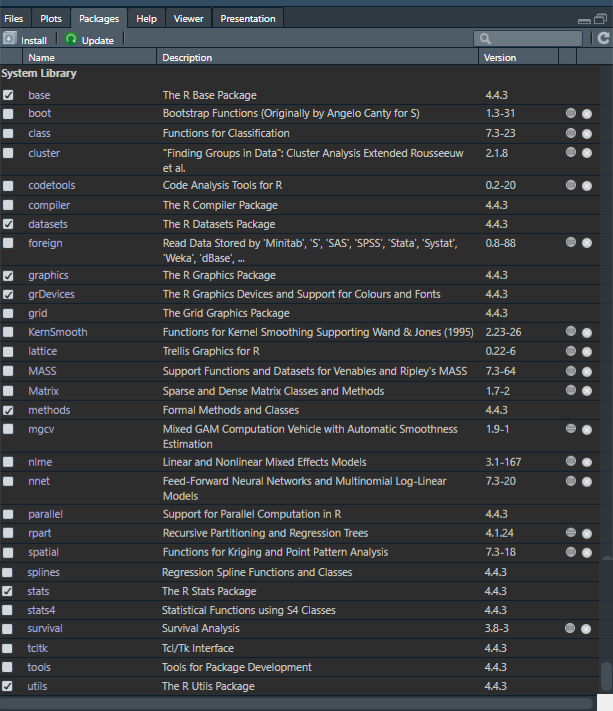
\includegraphics[width=0.75\linewidth,height=\textheight,keepaspectratio]{unidad_1/images/rbase_paquetes.png}
\end{center}

En la actualidad, existen más de 17.000 paquetes disponibles para una
amplia variedad de aplicaciones, número que crece mes a mes gracias a la
naturaleza \emph{open source} del lenguaje. Cualquier persona puede
desarrollar y compartir sus propios paquetes, aunque no todos llegan a
publicarse en el repositorio oficial CRAN (Comprehensive R Archive
Network), que actúa como principal fuente de distribución.

Los paquetes pueden descargarse directamente desde CRAN o instalarse a
partir de archivos comprimidos locales (como \texttt{.zip} o
\texttt{.tar.gz}). Una vez instalados, se los puede activar en cualquier
análisis.

\subsection{Dependencias}\label{dependencias}

En muchos casos, al utilizar un paquete, este necesita de otros para
funcionar correctamente. Esta relación se conoce como
\textbf{dependencia}, y es una característica central en el ecosistema
de R.

La mayoría de las funciones incluidas en los paquetes están
desarrolladas en el propio lenguaje R y, durante su construcción, es
habitual que recurran a funciones ya existentes en otros paquetes. Por
ejemplo, una función nueva puede hacer uso de una función auxiliar que
no pertenece al sistema base, sino a otro paquete externo.

Cuando intentamos ejecutar una función que depende de otras no
disponibles en nuestra instalación, R no podrá encontrar esas funciones
y nos devolverá un mensaje de error indicando que no reconoce el nombre
solicitado. Este tipo de errores suele alertar sobre funciones
``desconocidas'' o ``no encontradas'', lo que indica que falta instalar
o activar alguno de los paquetes requeridos.

Para evitar estos inconvenientes, R intenta resolver automáticamente las
dependencias cuando instalamos un paquete desde el repositorio oficial
CRAN. Si el paquete necesita otros para funcionar, el sistema detecta
esta relación y se encarga de instalar también aquellos paquetes
auxiliares. De todos modos, si alguno no se instala correctamente o no
se activa en la sesión, será necesario hacerlo de forma manual.

\section{Errores y advertencias}\label{errores-y-advertencias}

El lenguaje R es muy preciso en su sintaxis. Cometer errores al escribir
funciones u objetos es común durante el aprendizaje, y el intérprete de
R devuelve mensajes de error cuando detecta algo incorrecto.

Uno de los aspectos clave a tener en cuenta es que R \textbf{distingue
entre mayúsculas y minúsculas} (\emph{case sensitive}), por lo que no es
lo mismo escribir \texttt{a} que \texttt{A}.

Existen tres grupos de mensajes de error:

\begin{itemize}
\item
  Errores de sintaxis
\item
  Error de objeto no encontrado
\item
  Otros errores
\end{itemize}

\subsection{Errores de sintaxis}\label{errores-de-sintaxis}

Ocurre cuando R no puede interpretar una línea de código porque algo
está mal escrito. Los errores de sintaxis más frecuentes incluyen:

\begin{itemize}
\item
  Paréntesis, comas, comillas, corchetes o llaves mal colocados o
  ausentes.
\item
  Argumentos mal separados o incorrectamente definidos.
\end{itemize}

Por ejemplo la función \texttt{rep()} repite valores una cantidad de
veces. Tiene dos argumentos, \texttt{x} donde se coloca el valor a
repetir y \texttt{times} donde se define la cantidad de veces:

\begin{Shaded}
\begin{Highlighting}[]
\FunctionTok{rep}\NormalTok{(}\AttributeTok{x =} \DecValTok{3}\NormalTok{, }\AttributeTok{times =} \DecValTok{4}\NormalTok{) }\CommentTok{\# repetimos 4 veces 3 con rep()}
\end{Highlighting}
\end{Shaded}

\begin{verbatim}
[1] 3 3 3 3
\end{verbatim}

Si nos olvidamos de cerrar el paréntesis:

\begin{Shaded}
\begin{Highlighting}[]
\FunctionTok{rep}\NormalTok{(}\AttributeTok{x =} \DecValTok{3}\NormalTok{, }\AttributeTok{times =} \DecValTok{4}
\end{Highlighting}
\end{Shaded}

\begin{verbatim}
Error in parse(text = input): <text>:2:0: unexpected end of input
1: rep(x = 3, times = 4
   ^
\end{verbatim}

Si omitimos la coma entre argumentos:

\begin{Shaded}
\begin{Highlighting}[]
\FunctionTok{rep}\NormalTok{(}\AttributeTok{x =} \DecValTok{3} \AttributeTok{times =} \DecValTok{4}\NormalTok{)}
\end{Highlighting}
\end{Shaded}

\begin{verbatim}
Error in parse(text = input): <text>:1:11: unexpected symbol
1: rep(x = 3 times
              ^
\end{verbatim}

Si usamos un nombre de argumento no válido:

\begin{Shaded}
\begin{Highlighting}[]
\FunctionTok{rep}\NormalTok{(}\AttributeTok{y =} \DecValTok{3}\NormalTok{, }\AttributeTok{times =} \DecValTok{4}\NormalTok{)}
\end{Highlighting}
\end{Shaded}

\begin{verbatim}
Error in `rep()`:
! attempt to replicate an object of type 'symbol'
\end{verbatim}

Si escribimos mal el nombre de la función:

\begin{Shaded}
\begin{Highlighting}[]
\FunctionTok{rop}\NormalTok{(}\AttributeTok{x =} \DecValTok{3}\NormalTok{, }\AttributeTok{times =} \DecValTok{4}\NormalTok{)}
\end{Highlighting}
\end{Shaded}

\begin{verbatim}
Error in `rop()`:
! could not find function "rop"
\end{verbatim}

Este último error se asemeja a un error de objeto no encontrado, aunque
tiene origen en un problema de sintaxis.

Los mensajes de error en general y sobre todo al principio pueden
parecer extraños y difíciles de entender, pero con un poco de práctica
podemos inferir donde está el problema.

\subsection{Error de objeto no
encontrado}\label{error-de-objeto-no-encontrado}

Este tipo de error se produce cuando R no reconoce un objeto utilizado
en el código. Las causas más frecuentes incluyen:

\begin{itemize}
\item
  El nombre del objeto está mal escrito (por ejemplo, errores de
  sintaxis o uso incorrecto de mayúsculas/minúsculas).
\item
  El objeto pertenece a un paquete o archivo que no fue cargado.
\item
  Faltan comillas al declarar caracteres.
\item
  Otras causas similares.
\end{itemize}

Volvamos al ejemplo anterior, ahora repitiendo un valor tipo
\texttt{character}:

\begin{Shaded}
\begin{Highlighting}[]
\FunctionTok{rep}\NormalTok{(}\AttributeTok{x =} \StringTok{"A"}\NormalTok{, }\AttributeTok{times =} \DecValTok{4}\NormalTok{) }\CommentTok{\# repetimos 4 veces "A" con rep()}
\end{Highlighting}
\end{Shaded}

\begin{verbatim}
[1] "A" "A" "A" "A"
\end{verbatim}

Si olvidamos las comillas:

\begin{Shaded}
\begin{Highlighting}[]
\FunctionTok{rep}\NormalTok{(}\AttributeTok{x =}\NormalTok{ A, }\AttributeTok{times =} \DecValTok{4}\NormalTok{) }\CommentTok{\# repetimos 4 veces A con rep()}
\end{Highlighting}
\end{Shaded}

\begin{verbatim}
Error:
! object 'A' not found
\end{verbatim}

\subsection{Otros errores}\label{otros-errores}

Son aquellos que se generan por causas distintas a errores de sintaxis o
de objeto no encontrado. Por ejemplo:

\begin{Shaded}
\begin{Highlighting}[]
\StringTok{"x"} \SpecialCharTok{+} \DecValTok{10}
\end{Highlighting}
\end{Shaded}

\begin{verbatim}
Error in `"x" + 10`:
! non-numeric argument to binary operator
\end{verbatim}

El código anterior genera un mensaje de error porque intenta sumar
objetos de tipos incompatibles entre sí.

Veamos otro ejemplo:

\begin{Shaded}
\begin{Highlighting}[]
\FunctionTok{t.test}\NormalTok{(}\DecValTok{1}\NormalTok{)}
\end{Highlighting}
\end{Shaded}

\begin{verbatim}
Error in `t.test.default()`:
! not enough 'x' observations
\end{verbatim}

En este caso, el error se debe a que no hay suficientes observaciones
para realizar una prueba \(t\) de Student.

Otro caso frecuente ocurre cuando se intenta acceder a una posición
inexistente en un vector:

\begin{Shaded}
\begin{Highlighting}[]
\NormalTok{x }\OtherTok{\textless{}{-}} \FunctionTok{c}\NormalTok{(}\DecValTok{1}\NormalTok{, }\DecValTok{2}\NormalTok{, }\DecValTok{3}\NormalTok{)}
\NormalTok{x[[}\DecValTok{5}\NormalTok{]]}
\end{Highlighting}
\end{Shaded}

\begin{verbatim}
Error in `x[[5]]`:
! subscript out of bounds
\end{verbatim}

Este mensaje de error indica que el subíndice está fuera de los límites
del objeto (\texttt{subscript\ out\ of\ bounds}).

\subsection{Advertencias}\label{advertencias}

Las advertencia no son tan serias como un error, o al menos no lo
parece, ya que permiten el código se ejecute igual. Pero puede ocurrir
que ignorar una advertencia llegue a ser algo muy serio, si esto implica
que la salida de la función es equivocada.

Ignorar advertencias puede llevar a conclusiones erróneas, por lo que es
recomendable prestarles atención y entender su causa.

Por ejemplo:

\begin{Shaded}
\begin{Highlighting}[]
\FunctionTok{log}\NormalTok{(}\SpecialCharTok{{-}}\DecValTok{1}\NormalTok{)}
\end{Highlighting}
\end{Shaded}

\begin{verbatim}
Warning in log(-1): NaNs produced
\end{verbatim}

\begin{verbatim}
[1] NaN
\end{verbatim}

la función genera una advertencia porque el logaritmo de un número
negativo no está definido en los reales, y R devuelve un valor
\texttt{NaN} (\emph{Not a Number}).

\subsubsection{Resumiendo\ldots{}}\label{resumiendo}

\begin{center}
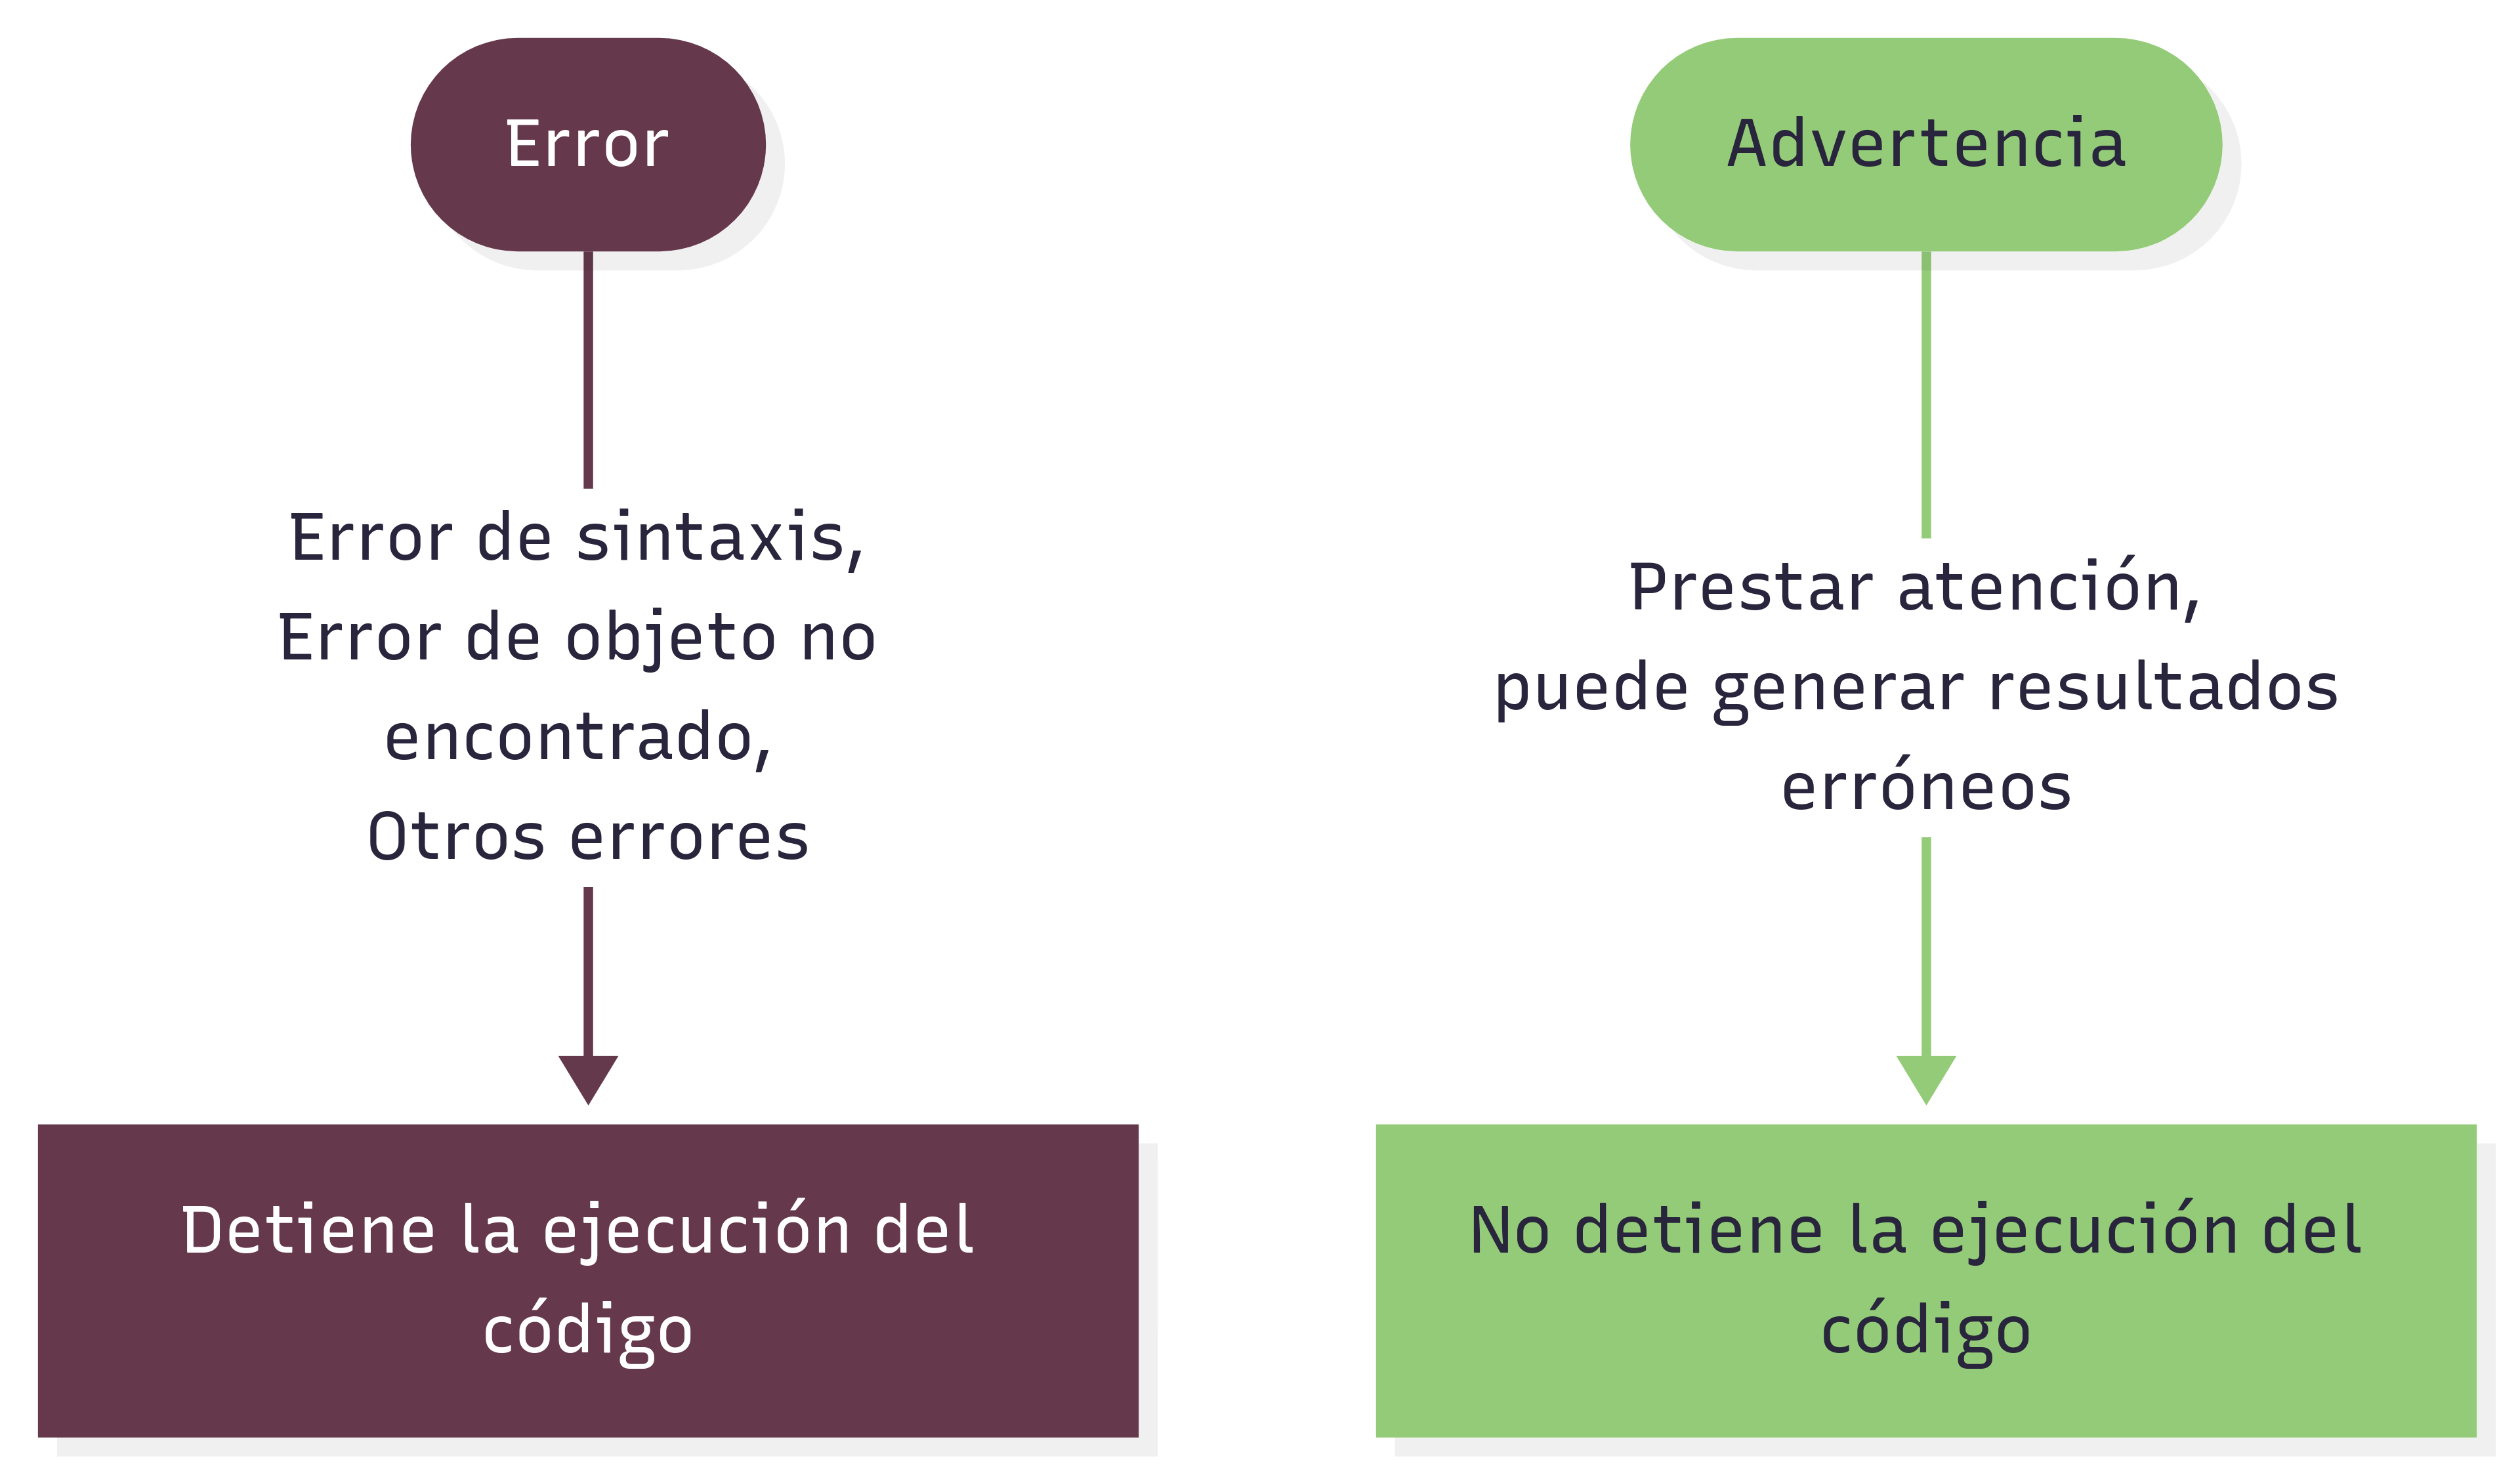
\includegraphics[width=0.7\linewidth,height=\textheight,keepaspectratio]{unidad_1/images/error_warning.png}
\end{center}

\section{Creación de objetos}\label{creaciuxf3n-de-objetos}

Todas las declaraciones donde se crean objetos usan el símbolo de
asignación \texttt{\textless{}-}:

\begin{Shaded}
\begin{Highlighting}[]
\NormalTok{nombre\_objeto }\OtherTok{\textless{}{-}}\NormalTok{ valor}
\end{Highlighting}
\end{Shaded}

Veámoslo en un ejemplo:

\begin{Shaded}
\begin{Highlighting}[]
\NormalTok{a }\OtherTok{\textless{}{-}} \DecValTok{1}
\end{Highlighting}
\end{Shaded}

En este caso asignamos el valor 1 al objeto \texttt{a}. El objeto
\texttt{a} es un vector de una posición (un solo valor). Si llamamos al
objeto, el intérprete devuelve el valor asignado previamente:

\begin{Shaded}
\begin{Highlighting}[]
\NormalTok{a}
\end{Highlighting}
\end{Shaded}

\begin{verbatim}
[1] 1
\end{verbatim}

Observemos que, además de devolvernos el valor, aparece delante un
número entre corchetes \texttt{{[}1{]}}. Este número es la ubicación o
\textbf{índice} del comienzo del objeto. En este caso, como el vector
tiene una sola posición, indica que el primer valor mostrado empieza en
la posición 1.

\section{Estructuras de datos}\label{estructuras-de-datos}

Los objetos contenedores de datos más simples pertenecen a cinco clases
atómicas, que son:

\begin{itemize}
\item
  \texttt{integer} (números enteros)
\item
  \texttt{numeric} (números reales)
\item
  \texttt{complex} (números complejos)
\item
  \texttt{character} (cadenas de caracteres)
\item
  \texttt{logical} (valores lógicos: \texttt{TRUE} o \texttt{FALSE})
\end{itemize}

\begin{center}
\pandocbounded{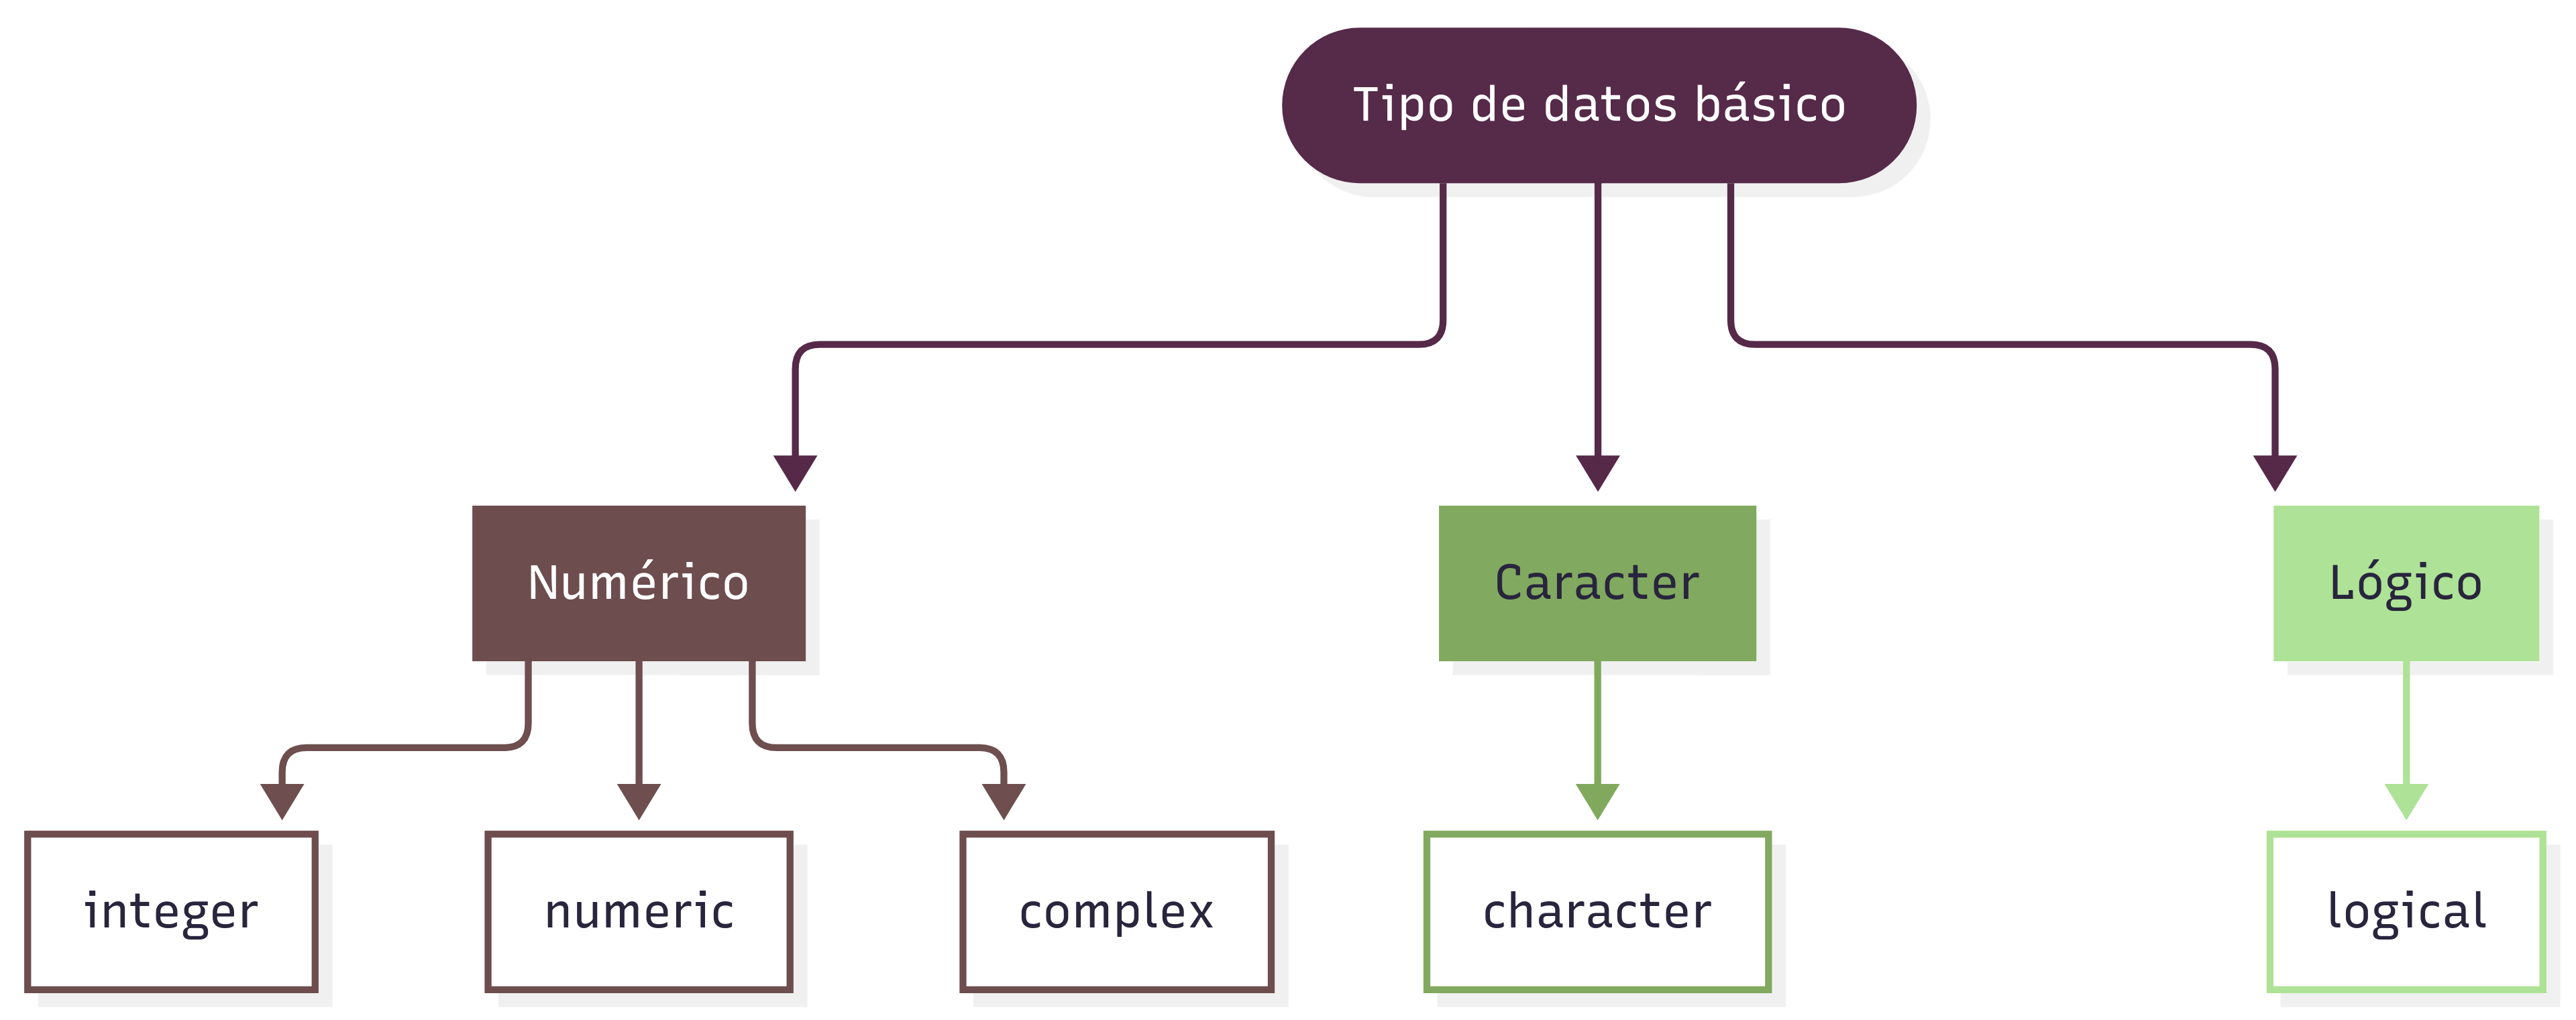
\includegraphics[keepaspectratio]{unidad_1/images/tipo_datos.png}}
\end{center}

Sin embargo, cada una de estas clases de datos no se encuentran de
manera aislada, sino encapsuladas dentro de la clase de objeto más
básica de R, a la que se denomina \textbf{vector}.

En RStudio, el sistema de colores ayuda a distinguir los tipos de
valores:

\begin{Shaded}
\begin{Highlighting}[]
\CommentTok{\# Número}
\DecValTok{1111}
\end{Highlighting}
\end{Shaded}

\begin{verbatim}
[1] 1111
\end{verbatim}

\begin{Shaded}
\begin{Highlighting}[]
\CommentTok{\# Caracter}
\StringTok{"esto es una cadena de texto"}
\end{Highlighting}
\end{Shaded}

\begin{verbatim}
[1] "esto es una cadena de texto"
\end{verbatim}

\begin{Shaded}
\begin{Highlighting}[]
\CommentTok{\# Lógico}
\ConstantTok{TRUE}
\end{Highlighting}
\end{Shaded}

\begin{verbatim}
[1] TRUE
\end{verbatim}

\begin{Shaded}
\begin{Highlighting}[]
\CommentTok{\# Objeto}
\NormalTok{a }\OtherTok{\textless{}{-}} \DecValTok{1}
\end{Highlighting}
\end{Shaded}

\subsection{Vectores}\label{vectores}

Un vector es un conjunto de valores (números o símbolos), del mismo tipo
ordenados de la forma (elemento 1, elemento 2, \ldots{} , elemento
\(n\)), donde \(n\) es la longitud o tamaño del vector.

Los atributos principales son:

\begin{itemize}
\item
  \textbf{Tipo}: puede ser \texttt{integer}, \texttt{numeric},
  \texttt{character}, \texttt{complex} o \texttt{logical}.
\item
  \textbf{Longitud}: cantidad de elementos que contiene el objeto,
\end{itemize}

El vector más simple contiene un solo dato, por ejemplo un vector de
longitud 1 y tipo \texttt{numeric}:

\begin{Shaded}
\begin{Highlighting}[]
\NormalTok{vec1 }\OtherTok{\textless{}{-}} \DecValTok{1}
\NormalTok{vec1}
\end{Highlighting}
\end{Shaded}

\begin{verbatim}
[1] 1
\end{verbatim}

Otro vector más grande por ejemplo podría ser \texttt{(1,\ 5,\ 2)}. En
este caso también es del tipo \texttt{numeric} pero tiene una longitud
de 3 elementos:

\begin{Shaded}
\begin{Highlighting}[]
\NormalTok{vec2 }\OtherTok{\textless{}{-}} \FunctionTok{c}\NormalTok{(}\DecValTok{1}\NormalTok{, }\DecValTok{5}\NormalTok{, }\DecValTok{2}\NormalTok{)}
\NormalTok{vec2}
\end{Highlighting}
\end{Shaded}

\begin{verbatim}
[1] 1 5 2
\end{verbatim}

Para concatenar elementos usamos la función \texttt{c()}, dentro de la
cual van los valores separados por comas. El orden de los elementos
importa, en nuestro ejemplo la primera posición la ocupa el 1, la
segunda el 5 y la tercera el 2. Si tuvieramos otro vector
\texttt{(5,\ 1,\ 2)}, no sería lo mismo porque los valores están
ordenados de forma diferente.

Para conocer la longitud del vector usamos:

\begin{Shaded}
\begin{Highlighting}[]
\FunctionTok{length}\NormalTok{(vec2)}
\end{Highlighting}
\end{Shaded}

\begin{verbatim}
[1] 3
\end{verbatim}

Nos informa que \texttt{vec2} tiene 3 elementos.

Para conocer el tipo de dato ejecutamos:

\begin{Shaded}
\begin{Highlighting}[]
\FunctionTok{class}\NormalTok{(vec2)}
\end{Highlighting}
\end{Shaded}

\begin{verbatim}
[1] "numeric"
\end{verbatim}

Podemos ver que los datos almacenados en este segundo ejemplo cumplen
con la definición en lo que respecta al tipo de dato, ya que cada
elemento es del mismo tipo (\texttt{numeric}).

Veamos un ejemplo de asignación de otro tipo de dato atómico, como es el
\texttt{character}:

\begin{Shaded}
\begin{Highlighting}[]
\NormalTok{vec3 }\OtherTok{\textless{}{-}} \StringTok{"Hola"}
\NormalTok{vec3}
\end{Highlighting}
\end{Shaded}

\begin{verbatim}
[1] "Hola"
\end{verbatim}

Siempre que escribamos contenido de tipo \texttt{character} debemos
hacerlo entre comillas. En este caso generamos el vector \texttt{vec3}
con el contenido \texttt{"Hola"}, que, a pesar de ser una palabra
compuesta de varios caracteres, dentro del vector \texttt{vec3} esta
ocupa una sola posición:

\begin{Shaded}
\begin{Highlighting}[]
\FunctionTok{length}\NormalTok{(vec3)}
\end{Highlighting}
\end{Shaded}

\begin{verbatim}
[1] 1
\end{verbatim}

Respecto al tipo de dato si usamos la función \texttt{class()}
tendremos:

\begin{Shaded}
\begin{Highlighting}[]
\FunctionTok{class}\NormalTok{(vec3)}
\end{Highlighting}
\end{Shaded}

\begin{verbatim}
[1] "character"
\end{verbatim}

\subsection{Factores}\label{factores}

Un factor es un objeto especialmente diseñado para contener datos
categóricos y se asocia particularmente con las \emph{variables
cualitativas}.

En su estructura interna está compuesto por dos vectores:

\begin{itemize}
\item
  Un vector de índices enteros.
\item
  Un vector de categorías (niveles) de tipo \texttt{character}, a los
  que hace referencia el primer vector.
\end{itemize}

Existen de dos tipos: factores nominales y factores ordinales. En el
caso del segundo se establece un orden en los niveles.

Normalmente, obtenemos un tipo \texttt{factor} de convertir un vector u
otro tipo de objeto con caracteres, pero para mostrar un ejemplo lo
realizamos con la función \texttt{factor()}:

\begin{Shaded}
\begin{Highlighting}[]
\NormalTok{factor1 }\OtherTok{\textless{}{-}} \FunctionTok{factor}\NormalTok{(}
  \AttributeTok{x =} \FunctionTok{c}\NormalTok{(}\StringTok{"a"}\NormalTok{, }\StringTok{"b"}\NormalTok{, }\StringTok{"a"}\NormalTok{, }\StringTok{"c"}\NormalTok{, }\StringTok{"b"}\NormalTok{, }\StringTok{"a"}\NormalTok{),}
  \AttributeTok{levels =} \FunctionTok{c}\NormalTok{(}\StringTok{"a"}\NormalTok{, }\StringTok{"b"}\NormalTok{, }\StringTok{"c"}\NormalTok{)}
\NormalTok{)}
\NormalTok{factor1}
\end{Highlighting}
\end{Shaded}

\begin{verbatim}
[1] a b a c b a
Levels: a b c
\end{verbatim}

Creamos el objeto \texttt{factor}1 con 6 elementos caracteres y tres
niveles sin orden.

Además de la practicidad de trabajar con factores, muchas funciones de R
requieren que las variables categóricas estén en formato factor para
funcionar correctamente.

\subsection{\texorpdfstring{\emph{Dataframe}}{Dataframe}}\label{dataframe}

Un \emph{dataframe} es un objeto diseñado para contener conjuntos de
datos y representa una estructura bidimensional similar a una tabla, con
filas y columnas. Cada columna puede almacenar elementos de distintos
tipos (por ejemplo, numéricos, de texto o lógicos), siempre que todos
tengan la misma longitud.

Las columnas suelen tener nombres únicos, lo que permite referenciarlas
fácilmente como si fueran variables individuales dentro del conjunto de
datos.

Este es el tipo de objeto que se utiliza habitualmente para almacenar
información importada desde archivos externos (por ejemplo, archivos de
texto separados por comas o planillas de Excel), y con el que más
frecuentemente trabajamos en los análisis.

Desde el punto de vista estructural, un \emph{dataframe} está compuesto
por una serie de vectores de igual longitud dispuestos verticalmente,
uno al lado del otro, conformando las columnas de la tabla.

Veamos un ejemplo:

\begin{Shaded}
\begin{Highlighting}[]
\CommentTok{\# Historia clínica}
\NormalTok{HC }\OtherTok{\textless{}{-}} \FunctionTok{c}\NormalTok{(}\StringTok{"F324"}\NormalTok{, }\StringTok{"G21"}\NormalTok{, }\StringTok{"G34"}\NormalTok{, }\StringTok{"F231"}\NormalTok{)}

\CommentTok{\# Edad}
\NormalTok{edad }\OtherTok{\textless{}{-}} \FunctionTok{c}\NormalTok{(}\DecValTok{34}\NormalTok{, }\DecValTok{32}\NormalTok{, }\DecValTok{34}\NormalTok{, }\DecValTok{54}\NormalTok{)}

\CommentTok{\# Sexo}
\NormalTok{sexo }\OtherTok{\textless{}{-}} \FunctionTok{c}\NormalTok{(}\StringTok{"M"}\NormalTok{, }\StringTok{"V"}\NormalTok{, }\StringTok{"V"}\NormalTok{, }\StringTok{"M"}\NormalTok{)}

\CommentTok{\# dataframe}
\NormalTok{df1 }\OtherTok{\textless{}{-}} \FunctionTok{data.frame}\NormalTok{(HC, edad, sexo)}

\NormalTok{df1}
\end{Highlighting}
\end{Shaded}

\begin{verbatim}
    HC edad sexo
1 F324   34    M
2  G21   32    V
3  G34   34    V
4 F231   54    M
\end{verbatim}

Creamos tres vectores con datos de supuestos individuos, su historia
clinica, la edad y el sexo. Luego mediante la función
\texttt{data.frame()} ``unimos'' esos vectores en forma vertical para
formar un \emph{dataframe} de 3 variables y 4 observaciones.

\begin{tcolorbox}[enhanced jigsaw, arc=.35mm, bottomrule=.15mm, breakable, colback=white, colframe=quarto-callout-warning-color-frame, left=2mm, leftrule=.75mm, opacityback=0, rightrule=.15mm, toprule=.15mm]
\begin{minipage}[t]{5.5mm}
\textcolor{quarto-callout-warning-color}{\faExclamationTriangle}
\end{minipage}%
\begin{minipage}[t]{\textwidth - 5.5mm}

Existen otras estructuras de datos que aparecen en la siguiente figura.
Las más habituales en nuestro trabajo son los vectores y los
\emph{dataframes}. Los factores serán necesarios cuando tengamos que
especificar distintos órdenes de niveles.

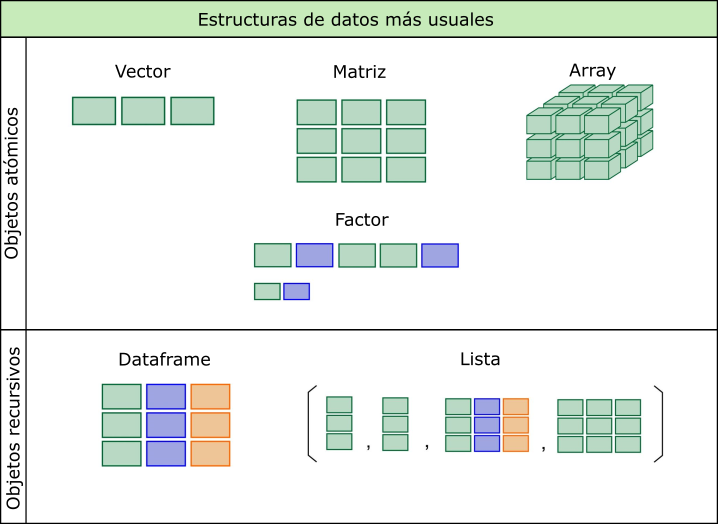
\includegraphics[width=6.25in,height=\textheight,keepaspectratio]{unidad_1/images/objetos_R.png}

\end{minipage}%
\end{tcolorbox}

\section{Operadores}\label{operadores}

Además de funciones, el lenguaje R cuenta con operadores de uso
relativamente intuitivo, que permiten realizar operaciones de diferentes
tipos con los objetos que contienen datos.

\subsection{Operadores aritméticos}\label{operadores-aritmuxe9ticos}

\begin{table}
\centering
\begin{tabular}[t]{l|l}
\hline
\cellcolor[HTML]{2f2e4e}{\textcolor{white}{Operador}} & \cellcolor[HTML]{2f2e4e}{\textcolor{white}{Descripción}}\\
\hline
+ & Suma\\
\hline
- & Resta\\
\hline
* & Multiplicación\\
\hline
/ & División\\
\hline
\textasciicircum{} & Potencia\\
\hline
\%\% & Módulo\\
\hline
\%/\% & División de enteros\\
\hline
\end{tabular}
\end{table}

Los operadores aritméticos se utilizan como si el lenguaje fuese una
calculadora:

\begin{Shaded}
\begin{Highlighting}[]
\CommentTok{\# Suma}
\DecValTok{2} \SpecialCharTok{+} \DecValTok{5}
\end{Highlighting}
\end{Shaded}

\begin{verbatim}
[1] 7
\end{verbatim}

\begin{Shaded}
\begin{Highlighting}[]
\CommentTok{\# Resta}
\DecValTok{3} \SpecialCharTok{{-}} \DecValTok{2}
\end{Highlighting}
\end{Shaded}

\begin{verbatim}
[1] 1
\end{verbatim}

\begin{Shaded}
\begin{Highlighting}[]
\CommentTok{\# Multiplicación}
\DecValTok{9} \SpecialCharTok{*} \DecValTok{3}
\end{Highlighting}
\end{Shaded}

\begin{verbatim}
[1] 27
\end{verbatim}

\begin{Shaded}
\begin{Highlighting}[]
\CommentTok{\# División}
\DecValTok{10} \SpecialCharTok{/} \DecValTok{2}
\end{Highlighting}
\end{Shaded}

\begin{verbatim}
[1] 5
\end{verbatim}

\begin{Shaded}
\begin{Highlighting}[]
\CommentTok{\# Potencia}
\DecValTok{5}\SpecialCharTok{\^{}}\DecValTok{2}
\end{Highlighting}
\end{Shaded}

\begin{verbatim}
[1] 25
\end{verbatim}

También se pueden hacer operaciones con los objetos que almacenan
valores numéricos:

\begin{Shaded}
\begin{Highlighting}[]
\NormalTok{a }\OtherTok{\textless{}{-}} \DecValTok{3}

\NormalTok{b }\OtherTok{\textless{}{-}} \DecValTok{6}

\NormalTok{(a }\SpecialCharTok{+}\NormalTok{ b) }\SpecialCharTok{*}\NormalTok{ b}
\end{Highlighting}
\end{Shaded}

\begin{verbatim}
[1] 54
\end{verbatim}

Y funciona con objetos con más de un elemento, aplicando aritmética
vectorial, donde las operaciones se realizan elemento a elemento:

\begin{Shaded}
\begin{Highlighting}[]
\NormalTok{a }\OtherTok{\textless{}{-}} \FunctionTok{c}\NormalTok{(}\DecValTok{1}\NormalTok{, }\DecValTok{2}\NormalTok{, }\DecValTok{3}\NormalTok{)}

\NormalTok{a }\SpecialCharTok{*} \DecValTok{3}
\end{Highlighting}
\end{Shaded}

\begin{verbatim}
[1] 3 6 9
\end{verbatim}

O bien, con operaciones entre los objetos, donde se realiza entre los
elementos de la misma posición:

\begin{Shaded}
\begin{Highlighting}[]
\NormalTok{a }\OtherTok{\textless{}{-}} \FunctionTok{c}\NormalTok{(}\DecValTok{1}\NormalTok{, }\DecValTok{2}\NormalTok{, }\DecValTok{3}\NormalTok{)}

\NormalTok{a }\SpecialCharTok{*}\NormalTok{ a}
\end{Highlighting}
\end{Shaded}

\begin{verbatim}
[1] 1 4 9
\end{verbatim}

\subsection{Operadores relacionales}\label{operadores-relacionales}

\begin{table}
\centering
\begin{tabular}[t]{l|l}
\hline
\cellcolor[HTML]{2f2e4e}{\textcolor{white}{Operador}} & \cellcolor[HTML]{2f2e4e}{\textcolor{white}{Descripción}}\\
\hline
< & Menor que\\
\hline
> & Mayor que\\
\hline
<= & Menor o igual que\\
\hline
>= & Mayor o igual que\\
\hline
== & Igual que\\
\hline
!= & No igual que\\
\hline
\end{tabular}
\end{table}

Habitualmente estos operadores se utilizan asiduamente en expresiones
para indicar relaciones entre valores.

Podemos ver su funcionamiento en el ejemplo siguiente:

\begin{Shaded}
\begin{Highlighting}[]
\NormalTok{a }\OtherTok{\textless{}{-}} \FunctionTok{c}\NormalTok{(}\DecValTok{3}\NormalTok{, }\DecValTok{8}\NormalTok{, }\DecValTok{2}\NormalTok{)}

\NormalTok{a }\SpecialCharTok{==} \FunctionTok{c}\NormalTok{(}\DecValTok{3}\NormalTok{, }\DecValTok{4}\NormalTok{, }\DecValTok{5}\NormalTok{)}
\end{Highlighting}
\end{Shaded}

\begin{verbatim}
[1]  TRUE FALSE FALSE
\end{verbatim}

El lenguaje evalúa las comparaciones que hace el operador relacional
igual (en este caso) y en aquellos valores que coinciden devuelve
\texttt{TRUE} y en los que no hay coincidencia devuelve \texttt{FALSE}.

Lo mismo sucede con los otros operadores relacionales:

\begin{Shaded}
\begin{Highlighting}[]
\NormalTok{a }\OtherTok{\textless{}{-}} \FunctionTok{c}\NormalTok{(}\DecValTok{4}\NormalTok{, }\DecValTok{8}\NormalTok{, }\DecValTok{10}\NormalTok{)}

\NormalTok{a }\SpecialCharTok{\textgreater{}} \DecValTok{8}
\end{Highlighting}
\end{Shaded}

\begin{verbatim}
[1] FALSE FALSE  TRUE
\end{verbatim}

\begin{Shaded}
\begin{Highlighting}[]
\NormalTok{a }\SpecialCharTok{\textless{}} \DecValTok{8}
\end{Highlighting}
\end{Shaded}

\begin{verbatim}
[1]  TRUE FALSE FALSE
\end{verbatim}

\begin{Shaded}
\begin{Highlighting}[]
\NormalTok{a }\SpecialCharTok{!=} \DecValTok{8}
\end{Highlighting}
\end{Shaded}

\begin{verbatim}
[1]  TRUE FALSE  TRUE
\end{verbatim}

\subsection{Operadores lógicos}\label{operadores-luxf3gicos}

\begin{table}
\centering
\begin{tabular}[t]{l|l}
\hline
\cellcolor[HTML]{2f2e4e}{\textcolor{white}{Operador}} & \cellcolor[HTML]{2f2e4e}{\textcolor{white}{Descripción}}\\
\hline
! & NOT\\
\hline
\& & AND booleano\\
\hline
\&\& & AND booleano para vectores de longitud 1\\
\hline
| & OR booleano\\
\hline
|| & OR booleano para vectores de longitud 1\\
\hline
\end{tabular}
\end{table}

Cuando queremos conectar algunas de las expresiones relacionales hacemos
uso de estos operadores lógicos típicos (AND, OR, NOT).

Para ejemplificar podemos hacer:

\begin{Shaded}
\begin{Highlighting}[]
\NormalTok{a }\OtherTok{\textless{}{-}} \FunctionTok{c}\NormalTok{(}\DecValTok{1}\SpecialCharTok{:}\DecValTok{8}\NormalTok{)}

\NormalTok{a}
\end{Highlighting}
\end{Shaded}

\begin{verbatim}
[1] 1 2 3 4 5 6 7 8
\end{verbatim}

\begin{Shaded}
\begin{Highlighting}[]
\NormalTok{(a }\SpecialCharTok{\textgreater{}} \DecValTok{3}\NormalTok{) }\SpecialCharTok{\&}\NormalTok{ (a }\SpecialCharTok{\textless{}} \DecValTok{7}\NormalTok{)}
\end{Highlighting}
\end{Shaded}

\begin{verbatim}
[1] FALSE FALSE FALSE  TRUE  TRUE  TRUE FALSE FALSE
\end{verbatim}

En el caso anterior usamos el operador \& como conector AND de dos
expresiones relacionales donde el lenguaje devuelve \texttt{TRUE} en el
rango mayor a 3 y menor a 7 (valores 4,5 y 6).

\section{Valores especiales}\label{valores-especiales}

Existen algunos valores especiales para datos con expresiones reservadas
en R, entre ellos encontramos los valores \texttt{NA}, \texttt{NaN},
\texttt{Inf} y \texttt{NULL}.

\begin{table}
\centering
\begin{tabular}[t]{l|l|l}
\hline
\cellcolor[HTML]{2f2e4e}{\textcolor{white}{Operador}} & \cellcolor[HTML]{2f2e4e}{\textcolor{white}{Significado}} & \cellcolor[HTML]{2f2e4e}{\textcolor{white}{Descripción}}\\
\hline
NA & Not available & Es la forma de expresar a los valores perdidos o faltantes (missing values)\\
\hline
NaN & Not a number & Utilizado para resultados de operaciones que devuelven error numérico\\
\hline
Inf & Infinity & Valor infinito (positivo)\\
\hline
-Inf & Infinity & Valor infinito (negativo)\\
\hline
NULL & Null & Valor nulo\\
\hline
\end{tabular}
\end{table}

El más relevante de estos valores especiales es el \texttt{NA} que sirve
para indicar que no hay valor en esa posición o elemento de un objeto.

\section{Secuencias regulares}\label{secuencias-regulares}

Además de concatenar elementos con la función \texttt{c()}, existen tres
formas comunes de generar secuencias regulares.

La primera es mediante un \textbf{operador secuencial} (\texttt{:}), que
genera una secuencia de enteros entre dos valores, ya sea en forma
ascendente o descendente:

\begin{Shaded}
\begin{Highlighting}[]
\DecValTok{1}\SpecialCharTok{:}\DecValTok{10}
\end{Highlighting}
\end{Shaded}

\begin{verbatim}
 [1]  1  2  3  4  5  6  7  8  9 10
\end{verbatim}

\begin{Shaded}
\begin{Highlighting}[]
\DecValTok{10}\SpecialCharTok{:}\DecValTok{1}
\end{Highlighting}
\end{Shaded}

\begin{verbatim}
 [1] 10  9  8  7  6  5  4  3  2  1
\end{verbatim}

La segunda forma es mediante la función \texttt{seq()}, cuyos argumentos
principales son \texttt{from}, \texttt{to} y \texttt{by}. Esta función
permite mayor flexibilidad:

\begin{Shaded}
\begin{Highlighting}[]
\FunctionTok{seq}\NormalTok{(}\AttributeTok{from =} \DecValTok{1}\NormalTok{, }\AttributeTok{to =} \DecValTok{20}\NormalTok{, }\AttributeTok{by =} \DecValTok{2}\NormalTok{)}
\end{Highlighting}
\end{Shaded}

\begin{verbatim}
 [1]  1  3  5  7  9 11 13 15 17 19
\end{verbatim}

El ejemplo anterior genera una secuencia de números que comienza en 1 y
llega hasta 20, avanzando de dos en dos.

Algunos otros ejemplos de la misma función:

\begin{Shaded}
\begin{Highlighting}[]
\FunctionTok{seq}\NormalTok{(}\AttributeTok{from =} \FloatTok{0.1}\NormalTok{, }\AttributeTok{to =} \FloatTok{0.9}\NormalTok{, }\AttributeTok{by =} \FloatTok{0.1}\NormalTok{)}
\end{Highlighting}
\end{Shaded}

\begin{verbatim}
[1] 0.1 0.2 0.3 0.4 0.5 0.6 0.7 0.8 0.9
\end{verbatim}

\begin{Shaded}
\begin{Highlighting}[]
\FunctionTok{seq}\NormalTok{(}\AttributeTok{from =} \SpecialCharTok{{-}}\DecValTok{5}\NormalTok{, }\AttributeTok{to =} \DecValTok{5}\NormalTok{, }\AttributeTok{by =} \DecValTok{1}\NormalTok{)}
\end{Highlighting}
\end{Shaded}

\begin{verbatim}
 [1] -5 -4 -3 -2 -1  0  1  2  3  4  5
\end{verbatim}

\begin{Shaded}
\begin{Highlighting}[]
\FunctionTok{seq}\NormalTok{(}\AttributeTok{from =} \DecValTok{300}\NormalTok{, }\AttributeTok{to =} \DecValTok{0}\NormalTok{, }\AttributeTok{by =} \SpecialCharTok{{-}}\DecValTok{50}\NormalTok{)}
\end{Highlighting}
\end{Shaded}

\begin{verbatim}
[1] 300 250 200 150 100  50   0
\end{verbatim}

La tercera opción es la función \texttt{rep()}, que permite duplicar
valores. Su forma más básica es \texttt{rep(x,\ times\ =\ n)}, donde se
repite el valor \texttt{x} la cantidad de veces indicada por \texttt{n}.

Algunos ejemplos:

\begin{Shaded}
\begin{Highlighting}[]
\FunctionTok{rep}\NormalTok{(}\AttributeTok{x =} \DecValTok{2}\NormalTok{, }\AttributeTok{times =} \DecValTok{5}\NormalTok{)}
\end{Highlighting}
\end{Shaded}

\begin{verbatim}
[1] 2 2 2 2 2
\end{verbatim}

\begin{Shaded}
\begin{Highlighting}[]
\CommentTok{\# combinada con el operador :}
\FunctionTok{rep}\NormalTok{(}\DecValTok{1}\SpecialCharTok{:}\DecValTok{4}\NormalTok{, }\DecValTok{5}\NormalTok{)}
\end{Highlighting}
\end{Shaded}

\begin{verbatim}
 [1] 1 2 3 4 1 2 3 4 1 2 3 4 1 2 3 4 1 2 3 4
\end{verbatim}

\begin{Shaded}
\begin{Highlighting}[]
\CommentTok{\# combinada con la función c()}
\FunctionTok{rep}\NormalTok{(}\FunctionTok{c}\NormalTok{(}\FloatTok{4.5}\NormalTok{, }\FloatTok{6.8}\NormalTok{, }\FloatTok{7.2}\NormalTok{), }\DecValTok{2}\NormalTok{)}
\end{Highlighting}
\end{Shaded}

\begin{verbatim}
[1] 4.5 6.8 7.2 4.5 6.8 7.2
\end{verbatim}

\section{Índices}\label{uxedndices}

R implementa una forma eficiente y flexible de acceder selectivamente a
elementos de un objeto basado en una indexación interna.

Para acceder a un índice se utiliza la notación de corchetes. Por
ejemplo, si tenemos un vector \texttt{x} con varios elementos y queremos
acceder al segundo, usamos \texttt{x{[}2{]}}.

Esta forma de indexar los elementos de los distintos objetos nos permite
realizar muchas operaciones desde el simple llamado, hasta seleccionar,
eliminar o modificar valores.

Veamos algunos ejemplos:

\begin{Shaded}
\begin{Highlighting}[]
\CommentTok{\# generamos un vector x con 5 letras}
\NormalTok{x }\OtherTok{\textless{}{-}} \FunctionTok{c}\NormalTok{(}\StringTok{"a"}\NormalTok{, }\StringTok{"b"}\NormalTok{, }\StringTok{"c"}\NormalTok{, }\StringTok{"d"}\NormalTok{, }\StringTok{"e"}\NormalTok{)}

\CommentTok{\# llamamos a la primer posición y nos devuelve su valor}
\NormalTok{x[}\DecValTok{1}\NormalTok{]}
\end{Highlighting}
\end{Shaded}

\begin{verbatim}
[1] "a"
\end{verbatim}

\begin{Shaded}
\begin{Highlighting}[]
\CommentTok{\# llamamos a la tercer posición y nos devuelve su valor}
\NormalTok{x[}\DecValTok{3}\NormalTok{]}
\end{Highlighting}
\end{Shaded}

\begin{verbatim}
[1] "c"
\end{verbatim}

\begin{Shaded}
\begin{Highlighting}[]
\CommentTok{\# llamamos a las posiciones 1 y 3 juntas mediante c()}
\NormalTok{x[}\FunctionTok{c}\NormalTok{(}\DecValTok{1}\NormalTok{, }\DecValTok{3}\NormalTok{)]}
\end{Highlighting}
\end{Shaded}

\begin{verbatim}
[1] "a" "c"
\end{verbatim}

\begin{Shaded}
\begin{Highlighting}[]
\CommentTok{\# llamamos a las posiciones menos la 1 y la 4}
\NormalTok{x[}\SpecialCharTok{{-}}\FunctionTok{c}\NormalTok{(}\DecValTok{1}\NormalTok{, }\DecValTok{4}\NormalTok{)]}
\end{Highlighting}
\end{Shaded}

\begin{verbatim}
[1] "b" "c" "e"
\end{verbatim}

\begin{Shaded}
\begin{Highlighting}[]
\CommentTok{\# creamos otro vector y con los valores 1,2 y 5}
\NormalTok{y }\OtherTok{\textless{}{-}} \FunctionTok{c}\NormalTok{(}\DecValTok{1}\NormalTok{, }\DecValTok{2}\NormalTok{, }\DecValTok{5}\NormalTok{)}

\CommentTok{\# utilizamos el vector y como índice}
\NormalTok{x[y]}
\end{Highlighting}
\end{Shaded}

\begin{verbatim}
[1] "a" "b" "e"
\end{verbatim}

\begin{Shaded}
\begin{Highlighting}[]
\CommentTok{\# asignamos el valor “h” a la posición 2 del vector x}
\NormalTok{x[}\DecValTok{2}\NormalTok{] }\OtherTok{\textless{}{-}} \StringTok{"h"}

\NormalTok{x}
\end{Highlighting}
\end{Shaded}

\begin{verbatim}
[1] "a" "h" "c" "d" "e"
\end{verbatim}

\begin{Shaded}
\begin{Highlighting}[]
\CommentTok{\# creamos el vector z eliminando la posición 5 de x}
\NormalTok{z }\OtherTok{\textless{}{-}}\NormalTok{ x[}\SpecialCharTok{{-}}\DecValTok{5}\NormalTok{]}

\NormalTok{z}
\end{Highlighting}
\end{Shaded}

\begin{verbatim}
[1] "a" "h" "c" "d"
\end{verbatim}

Estos ejemplos muestran las múltiples posibilidades que ofrece el uso de
índices para manipular objetos en R, lo que hace al lenguaje muy
poderoso y versátil.

Cuando se aplican índices a estructuras bidimensionales, como matrices o
\emph{dataframes}, la notación general es:

\begin{Shaded}
\begin{Highlighting}[]
\NormalTok{nombre[índice de fila, índice de columna]}
\end{Highlighting}
\end{Shaded}

\section{Gestión de factores}\label{gestiuxf3n-de-factores}

Al presentar las distintas estructuras de datos mencionamos que los
factores suelen generarse a partir de vectores u otros objetos de tipo
carácter.

Para entender cómo funcionan, partamos de un vector con datos
categóricos:

\begin{Shaded}
\begin{Highlighting}[]
\NormalTok{respuesta }\OtherTok{\textless{}{-}} \FunctionTok{c}\NormalTok{(}\StringTok{"Si"}\NormalTok{, }\StringTok{"No"}\NormalTok{, }\StringTok{"No"}\NormalTok{, }\StringTok{"Si"}\NormalTok{, }\StringTok{"Si"}\NormalTok{, }\StringTok{"Si"}\NormalTok{, }\StringTok{"No"}\NormalTok{)}
\end{Highlighting}
\end{Shaded}

Creamos un vector llamado \texttt{respuesta} con 7 elementos de tipo
carácter, en el que se repiten las categorías \texttt{"Si"} y
\texttt{"No"}.

Podemos confirmar que se trata de un vector y que su contenido es de
tipo carácter:

\begin{Shaded}
\begin{Highlighting}[]
\CommentTok{\# preguntamos si sexo es un vector}
\FunctionTok{is.vector}\NormalTok{(respuesta)}
\end{Highlighting}
\end{Shaded}

\begin{verbatim}
[1] TRUE
\end{verbatim}

\begin{Shaded}
\begin{Highlighting}[]
\CommentTok{\# visualizamos el tipo de dato de sexo}
\FunctionTok{class}\NormalTok{(respuesta)}
\end{Highlighting}
\end{Shaded}

\begin{verbatim}
[1] "character"
\end{verbatim}

Para crear un factor a partir de este vector debemos utilizar la función
\texttt{factor()}:

\begin{Shaded}
\begin{Highlighting}[]
\NormalTok{respuesta }\OtherTok{\textless{}{-}} \FunctionTok{factor}\NormalTok{(respuesta)}

\NormalTok{respuesta}
\end{Highlighting}
\end{Shaded}

\begin{verbatim}
[1] Si No No Si Si Si No
Levels: No Si
\end{verbatim}

En la salida observamos los siete elementos y, debajo, una línea con los
niveles del factor, indicados por \texttt{Levels}. Estos niveles son
identificados automáticamente.

Podemos verificar cómo cambió el tipo de objeto:

\begin{Shaded}
\begin{Highlighting}[]
\CommentTok{\# preguntamos si respuesta es un vector}
\FunctionTok{is.vector}\NormalTok{(respuesta)}
\end{Highlighting}
\end{Shaded}

\begin{verbatim}
[1] FALSE
\end{verbatim}

\begin{Shaded}
\begin{Highlighting}[]
\CommentTok{\# preguntamos si respuesta es un factor}
\FunctionTok{is.factor}\NormalTok{(respuesta)}
\end{Highlighting}
\end{Shaded}

\begin{verbatim}
[1] TRUE
\end{verbatim}

\begin{Shaded}
\begin{Highlighting}[]
\CommentTok{\# visualizamos el tipo de dato de respuesta}
\FunctionTok{class}\NormalTok{(respuesta)}
\end{Highlighting}
\end{Shaded}

\begin{verbatim}
[1] "factor"
\end{verbatim}

Aunque visualmente vemos palabras, internamente R trata al factor como
un tipo especial basado en números. ¿Por qué sucede esto? Veámoslo con
más detalle:

\begin{Shaded}
\begin{Highlighting}[]
\FunctionTok{str}\NormalTok{(respuesta)}
\end{Highlighting}
\end{Shaded}

\begin{verbatim}
 Factor w/ 2 levels "No","Si": 2 1 1 2 2 2 1
\end{verbatim}

La función \texttt{str()} devuelve la estructura interna del objeto. En
este caso, muestra que \texttt{respuesta} tiene dos niveles y que cada
elemento del vector es representado por un número (1 o 2), donde
\texttt{1} corresponde a \texttt{"No"} y \texttt{2} a \texttt{"Si"}.

Esto significa que la estructura de los factores está compuesta por dos
vectores: uno numérico que funciona como índice de enteros, que
sustituye al vector de caracteres original, y el otro es un vector de
caracteres, que contiene los niveles o categorías, a los que hace
referencia el primer vector.

Para ver solo los niveles o categorías del factor podemos usar:

\begin{Shaded}
\begin{Highlighting}[]
\FunctionTok{levels}\NormalTok{(respuesta)}
\end{Highlighting}
\end{Shaded}

\begin{verbatim}
[1] "No" "Si"
\end{verbatim}

En los factores nominales donde no importa el orden, la función
\texttt{factor()} implementa el orden alfabético para determinar a qué
índice numérico pertenece cada categoría. Es claro en el ejemplo que a
\texttt{No} le asigna el \texttt{1} y a \texttt{Si} el \texttt{2}.

Pero si nos encontramos frente a una variable cualitativa ordinal vamos
a necesitar indicarle a la función cual es el orden de las categorías.

Vamos al siguiente ejemplo:

\begin{Shaded}
\begin{Highlighting}[]
\NormalTok{salud }\OtherTok{\textless{}{-}} \FunctionTok{c}\NormalTok{(}\DecValTok{4}\NormalTok{, }\DecValTok{3}\NormalTok{, }\DecValTok{1}\NormalTok{, }\DecValTok{3}\NormalTok{, }\DecValTok{2}\NormalTok{, }\DecValTok{2}\NormalTok{, }\DecValTok{3}\NormalTok{, }\DecValTok{3}\NormalTok{, }\DecValTok{1}\NormalTok{)}
\NormalTok{salud}
\end{Highlighting}
\end{Shaded}

\begin{verbatim}
[1] 4 3 1 3 2 2 3 3 1
\end{verbatim}

Tenemos en el vector salud algunos códigos numéricos que representan
nivel de salud de personas registradas por una encuesta donde \texttt{1}
significa mala salud, \texttt{2} regular, \texttt{3} buena y \texttt{4}
muy buena.

Procedemos a crear el factor \texttt{nivsalud} a partir de este vector:

\begin{Shaded}
\begin{Highlighting}[]
\NormalTok{nivsalud }\OtherTok{\textless{}{-}} \FunctionTok{factor}\NormalTok{(}
\NormalTok{  salud,}
  \AttributeTok{label =} \FunctionTok{c}\NormalTok{(}\StringTok{"Mala"}\NormalTok{, }\StringTok{"Regular"}\NormalTok{, }\StringTok{"Buena"}\NormalTok{, }\StringTok{"Muy buena"}\NormalTok{),}
  \AttributeTok{levels =} \DecValTok{1}\SpecialCharTok{:}\DecValTok{4}
\NormalTok{)}

\NormalTok{nivsalud}
\end{Highlighting}
\end{Shaded}

\begin{verbatim}
[1] Muy buena Buena     Mala      Buena     Regular   Regular   Buena    
[8] Buena     Mala     
Levels: Mala Regular Buena Muy buena
\end{verbatim}

Aquí utilizamos dos argumentos adicionales:

\begin{itemize}
\item
  \texttt{labels}: define las etiquetas que queremos mostrar para cada
  categoría.
\item
  \texttt{levels}: indica el orden de los niveles originales (en este
  caso, 1 a 4).
\end{itemize}

Aquí es necesario definir estos argumentos porque, a diferencia del
factor \texttt{respuesta}, el vector \texttt{salud} contiene números en
lugar de las palabras correspondientes a las categorías.

Hasta aquí hemos creado un factor pero si miramos sus niveles no
encontraremos señales que sigan un orden específico:

\begin{Shaded}
\begin{Highlighting}[]
\FunctionTok{levels}\NormalTok{(nivsalud)}
\end{Highlighting}
\end{Shaded}

\begin{verbatim}
[1] "Mala"      "Regular"   "Buena"     "Muy buena"
\end{verbatim}

Sin embargo, aún no hemos definido un \textbf{orden} explícito entre las
categorías. Para hacerlo, agregamos el argumento
\texttt{ordered\ =\ TRUE}:

\begin{Shaded}
\begin{Highlighting}[]
\NormalTok{nivsalud }\OtherTok{\textless{}{-}} \FunctionTok{factor}\NormalTok{(}
\NormalTok{  salud,}
  \AttributeTok{label =} \FunctionTok{c}\NormalTok{(}\StringTok{"Mala"}\NormalTok{, }\StringTok{"Regular"}\NormalTok{, }\StringTok{"Buena"}\NormalTok{, }\StringTok{"Muy buena"}\NormalTok{),}
  \AttributeTok{levels =} \DecValTok{1}\SpecialCharTok{:}\DecValTok{4}\NormalTok{,}
  \AttributeTok{ordered =} \ConstantTok{TRUE}
\NormalTok{)}

\NormalTok{nivsalud}
\end{Highlighting}
\end{Shaded}

\begin{verbatim}
[1] Muy buena Buena     Mala      Buena     Regular   Regular   Buena    
[8] Buena     Mala     
Levels: Mala < Regular < Buena < Muy buena
\end{verbatim}

Al incorporar este argumento, estamos diciendo que los niveles tienen
orden natural. Esto puede observarse en la salida donde se muestra que
\texttt{"Mala"} \textless{} \texttt{"Regular"} \textless{}
\texttt{"Buena"} \textless{} \texttt{"Muy\ buena"}.

\section{\texorpdfstring{Gestión de
\emph{dataframes}}{Gestión de dataframes}}\label{gestiuxf3n-de-dataframes}

En R, la estructura utilizada para almacenar datos provenientes de
fuentes externas (como archivos .csv, planillas de cálculo, bases SQL,
etc.) es el \emph{dataframe}.

A modo de ejemplo, vamos a construir un \emph{dataframe} llamado
\texttt{datos} con 4 variables y 5 observaciones. Las variables serán:

\begin{itemize}
\item
  \texttt{id}: identificador numérico entero y correlativo.
\item
  \texttt{edad}: edad en años.
\item
  \texttt{sexo}: codificado como \texttt{"V"} para varón y \texttt{"M"}
  para mujer.
\item
  \texttt{trabaja}: variable lógica, donde \texttt{TRUE} (\texttt{T})
  representa que la persona trabaja y \texttt{FALSE} (\texttt{F}) que no
  lo hace.
\end{itemize}

\begin{Shaded}
\begin{Highlighting}[]
\CommentTok{\# construimos el vector id}
\NormalTok{id }\OtherTok{\textless{}{-}} \DecValTok{1}\SpecialCharTok{:}\DecValTok{5}

\CommentTok{\# construimos el vector edad}
\NormalTok{edad }\OtherTok{\textless{}{-}} \FunctionTok{c}\NormalTok{(}\DecValTok{23}\NormalTok{, }\DecValTok{43}\NormalTok{, }\DecValTok{12}\NormalTok{, }\DecValTok{65}\NormalTok{, }\DecValTok{37}\NormalTok{)}

\CommentTok{\# construimos el vector sexo}
\NormalTok{sexo }\OtherTok{\textless{}{-}} \FunctionTok{c}\NormalTok{(}\StringTok{"V"}\NormalTok{, }\StringTok{"M"}\NormalTok{, }\StringTok{"M"}\NormalTok{, }\StringTok{"V"}\NormalTok{, }\StringTok{"M"}\NormalTok{)}

\CommentTok{\# construimos el vector trabaja}
\NormalTok{trabaja }\OtherTok{\textless{}{-}} \FunctionTok{c}\NormalTok{(T, T, F, F, T)}

\CommentTok{\# construimos el dataframe datos}
\NormalTok{datos }\OtherTok{\textless{}{-}} \FunctionTok{data.frame}\NormalTok{(id, edad, sexo, trabaja)}
\end{Highlighting}
\end{Shaded}

Aunque para el ejemplo construimos un \emph{dataframe} manualmente, lo
habitual en la práctica es leer archivos externos que se importan
directamente como \emph{dataframes}.

Algunas de las funciones generales que podemos aplicar son:

\begin{Shaded}
\begin{Highlighting}[]
\CommentTok{\# pedimos el número de columnas (variables)}
\FunctionTok{ncol}\NormalTok{(datos)}
\end{Highlighting}
\end{Shaded}

\begin{verbatim}
[1] 4
\end{verbatim}

\begin{Shaded}
\begin{Highlighting}[]
\CommentTok{\# pedimos el número de filas (registros u observaciones)}
\FunctionTok{nrow}\NormalTok{(datos)}
\end{Highlighting}
\end{Shaded}

\begin{verbatim}
[1] 5
\end{verbatim}

\begin{Shaded}
\begin{Highlighting}[]
\CommentTok{\# pedimos las dimensiones del dataframe (observaciones,variables)}
\FunctionTok{dim}\NormalTok{(datos)}
\end{Highlighting}
\end{Shaded}

\begin{verbatim}
[1] 5 4
\end{verbatim}

También podemos visualizar como se compone el objeto \texttt{datos}
aplicando \texttt{str()} que devuelve la estructura interna de cualquier
objeto en R.

\begin{Shaded}
\begin{Highlighting}[]
\FunctionTok{str}\NormalTok{(datos)}
\end{Highlighting}
\end{Shaded}

\begin{verbatim}
'data.frame':   5 obs. of  4 variables:
 $ id     : int  1 2 3 4 5
 $ edad   : num  23 43 12 65 37
 $ sexo   : chr  "V" "M" "M" "V" ...
 $ trabaja: logi  TRUE TRUE FALSE FALSE TRUE
\end{verbatim}

Esta salida nos informa que:

\begin{itemize}
\item
  \texttt{datos} es un \emph{dataframe} con 5 observaciones y 4
  variables.
\item
  \texttt{id} es un entero (\texttt{int}).
\item
  \texttt{edad} es numérica (\texttt{num}).
\item
  \texttt{sexo} es de tipo carácter (\texttt{chr}).
\item
  \texttt{trabaja} es lógica (\texttt{logi}).
\end{itemize}

Además, \texttt{str()} muestra los primeros valores de cada variable,
que en este caso son todos, ya que el \emph{dataframe} tiene solo 5
registros.

Cuando necesitemos llamar al contenido de alguna columna o variable del
\emph{dataframe}, utilizamos la siguiente notación:

\begin{Shaded}
\begin{Highlighting}[]
\NormalTok{nombre\_del\_dataframe}\SpecialCharTok{$}\NormalTok{nombre\_de\_la\_variable}
\end{Highlighting}
\end{Shaded}

Por ejemplo, si queremos mostrar el contenido de la variable
\texttt{sexo} del objeto \texttt{datos} hacemos:

\begin{Shaded}
\begin{Highlighting}[]
\NormalTok{datos}\SpecialCharTok{$}\NormalTok{sexo}
\end{Highlighting}
\end{Shaded}

\begin{verbatim}
[1] "V" "M" "M" "V" "M"
\end{verbatim}

Esto devuelve todos los valores de la variable \texttt{sexo}.

También podemos acceder a los elementos del \emph{dataframe} usando
\textbf{indexación por filas y columnas}:

\begin{Shaded}
\begin{Highlighting}[]
\CommentTok{\# pedimos la tercer variable (sexo)}
\NormalTok{datos[, }\DecValTok{3}\NormalTok{]}
\end{Highlighting}
\end{Shaded}

\begin{verbatim}
[1] "V" "M" "M" "V" "M"
\end{verbatim}

Observemos que las dos salidas son idénticas, dado que muestran todas
las observaciones de la variable \texttt{sexo}, aunque la solicitud sea
de manera diferente.

Algunos otros ejemplos de uso de índices:

\begin{Shaded}
\begin{Highlighting}[]
\CommentTok{\# observación 1 de la variable 2}
\NormalTok{datos[}\DecValTok{1}\NormalTok{, }\DecValTok{2}\NormalTok{]}
\end{Highlighting}
\end{Shaded}

\begin{verbatim}
[1] 23
\end{verbatim}

\begin{Shaded}
\begin{Highlighting}[]
\CommentTok{\# observación 4 de todas las variables}
\NormalTok{datos[}\DecValTok{4}\NormalTok{, ]}
\end{Highlighting}
\end{Shaded}

\begin{verbatim}
  id edad sexo trabaja
4  4   65    V   FALSE
\end{verbatim}

\begin{Shaded}
\begin{Highlighting}[]
\CommentTok{\# observación 1,2 y 3 de la variable 3}
\NormalTok{datos[}\DecValTok{1}\SpecialCharTok{:}\DecValTok{3}\NormalTok{, }\DecValTok{3}\NormalTok{]}
\end{Highlighting}
\end{Shaded}

\begin{verbatim}
[1] "V" "M" "M"
\end{verbatim}

\begin{Shaded}
\begin{Highlighting}[]
\CommentTok{\# observación 5 de las variables 1 y 4}
\NormalTok{datos[}\DecValTok{5}\NormalTok{, }\FunctionTok{c}\NormalTok{(}\DecValTok{1}\NormalTok{, }\DecValTok{4}\NormalTok{)]}
\end{Highlighting}
\end{Shaded}

\begin{verbatim}
  id trabaja
5  5    TRUE
\end{verbatim}

Por último, vamos podemos mostrar y gestionar los nombres de las
variables con la función \texttt{names()}:

\begin{Shaded}
\begin{Highlighting}[]
\FunctionTok{names}\NormalTok{(datos)}
\end{Highlighting}
\end{Shaded}

\begin{verbatim}
[1] "id"      "edad"    "sexo"    "trabaja"
\end{verbatim}

\section{Fórmulas}\label{fuxf3rmulas}

En R, las fórmulas se utilizan principalmente para describir modelos
estadísticos, y las vamos a emplear a lo largo de toda la cursada.

Las fórmulas se escriben utilizando operadores como
\texttt{\textasciitilde{}}, \texttt{+}, \texttt{*}, entre otros. Se usan
para especificar modelos como regresiones, ANOVA, pruebas de hipótesis
y, en algunos casos, también para generar ciertos tipos de gráficos.

\subsubsection{Formula genérica}\label{formula-genuxe9rica}

Aquí la formula está dada por el operador \texttt{\textasciitilde{}}, a
la izquierda está la variable de respuesta o dependiente, a la derecha
la o las variables explicativas o independientes. El esquema general es
el siguiente:

\begin{Shaded}
\begin{Highlighting}[]
\NormalTok{variable\_dependiente }\SpecialCharTok{\textasciitilde{}}\NormalTok{ variable}
\NormalTok{independiente}
\end{Highlighting}
\end{Shaded}

El símbolo \texttt{\textasciitilde{}} (llamado virgulilla) puede
interpretarse como \emph{``es modelada por''} o \emph{``en función
de''}.

Por ejemplo, en una regresión lineal se utiliza la función base
\texttt{lm()} y el argumento principal de esta función es una formula:

\begin{Shaded}
\begin{Highlighting}[]
\NormalTok{regresion\_lineal }\OtherTok{\textless{}{-}} \FunctionTok{lm}\NormalTok{(variable\_respuesta }\SpecialCharTok{\textasciitilde{}}\NormalTok{ variable\_explicativa, }\AttributeTok{data =}\NormalTok{ datos)}
\end{Highlighting}
\end{Shaded}

Además de la fórmula, la función \texttt{lm()} incluye el argumento
\texttt{data\ =}, que es fundamental: allí se le indica a R el
\emph{dataframe} en el que debe buscar las variables involucradas en el
modelo.

La siguiente tabla muestra los usos de los los operadores más comunes
dentro de una formula:

\begin{table}
\centering
\begin{tabular}[t]{l|l|l}
\hline
\cellcolor[HTML]{2f2e4e}{\textcolor{white}{Operador}} & \cellcolor[HTML]{2f2e4e}{\textcolor{white}{Ejemplo}} & \cellcolor[HTML]{2f2e4e}{\textcolor{white}{Descripción}}\\
\hline
+ & +x & Incluye la variable x\\
\hline
- & -x & Excluye la variable x\\
\hline
: & x : z & Incluye la interacción de la variable x con z\\
\hline
* & x * z & Incluye ambas variables y la interacción entre ellas\\
\hline
\end{tabular}
\end{table}

\chapter{Primeros pasos y
generalidades}\label{primeros-pasos-y-generalidades}

\begin{figure}[H]

{\centering 
\includegraphics[width=5.20833in,height=3.125in]{unidad_1/images/cracked_setwd.png}

}

\caption{Artwork por @allison\_horst}

\end{figure}%

\section{Introducción a RStudio}\label{introducciuxf3n-a-rstudio}

RStudio Desktop
\href{https://posit.co/products/open-source/rstudio/}{(2025, Posit
Software)} es un \textbf{entorno de desarrollo integrado} (\emph{IDE},
por sus siglas en inglés) diseñado específicamente para trabajar con el
lenguaje R.

Es una herramienta \textbf{multiplataforma y de código abierto} que
facilita la programación, el análisis de datos y la elaboración de
informes científicos. Ofrece una integración fluida con otros
componentes del ecosistema de R, como R Markdown, Quarto, control de
versiones (por ejemplo, Git) y la gestión de proyectos.

RStudio presenta una interfaz unificada compuesta por distintos paneles,
lo que permite organizar el trabajo de forma clara y eficiente:

\begin{center}
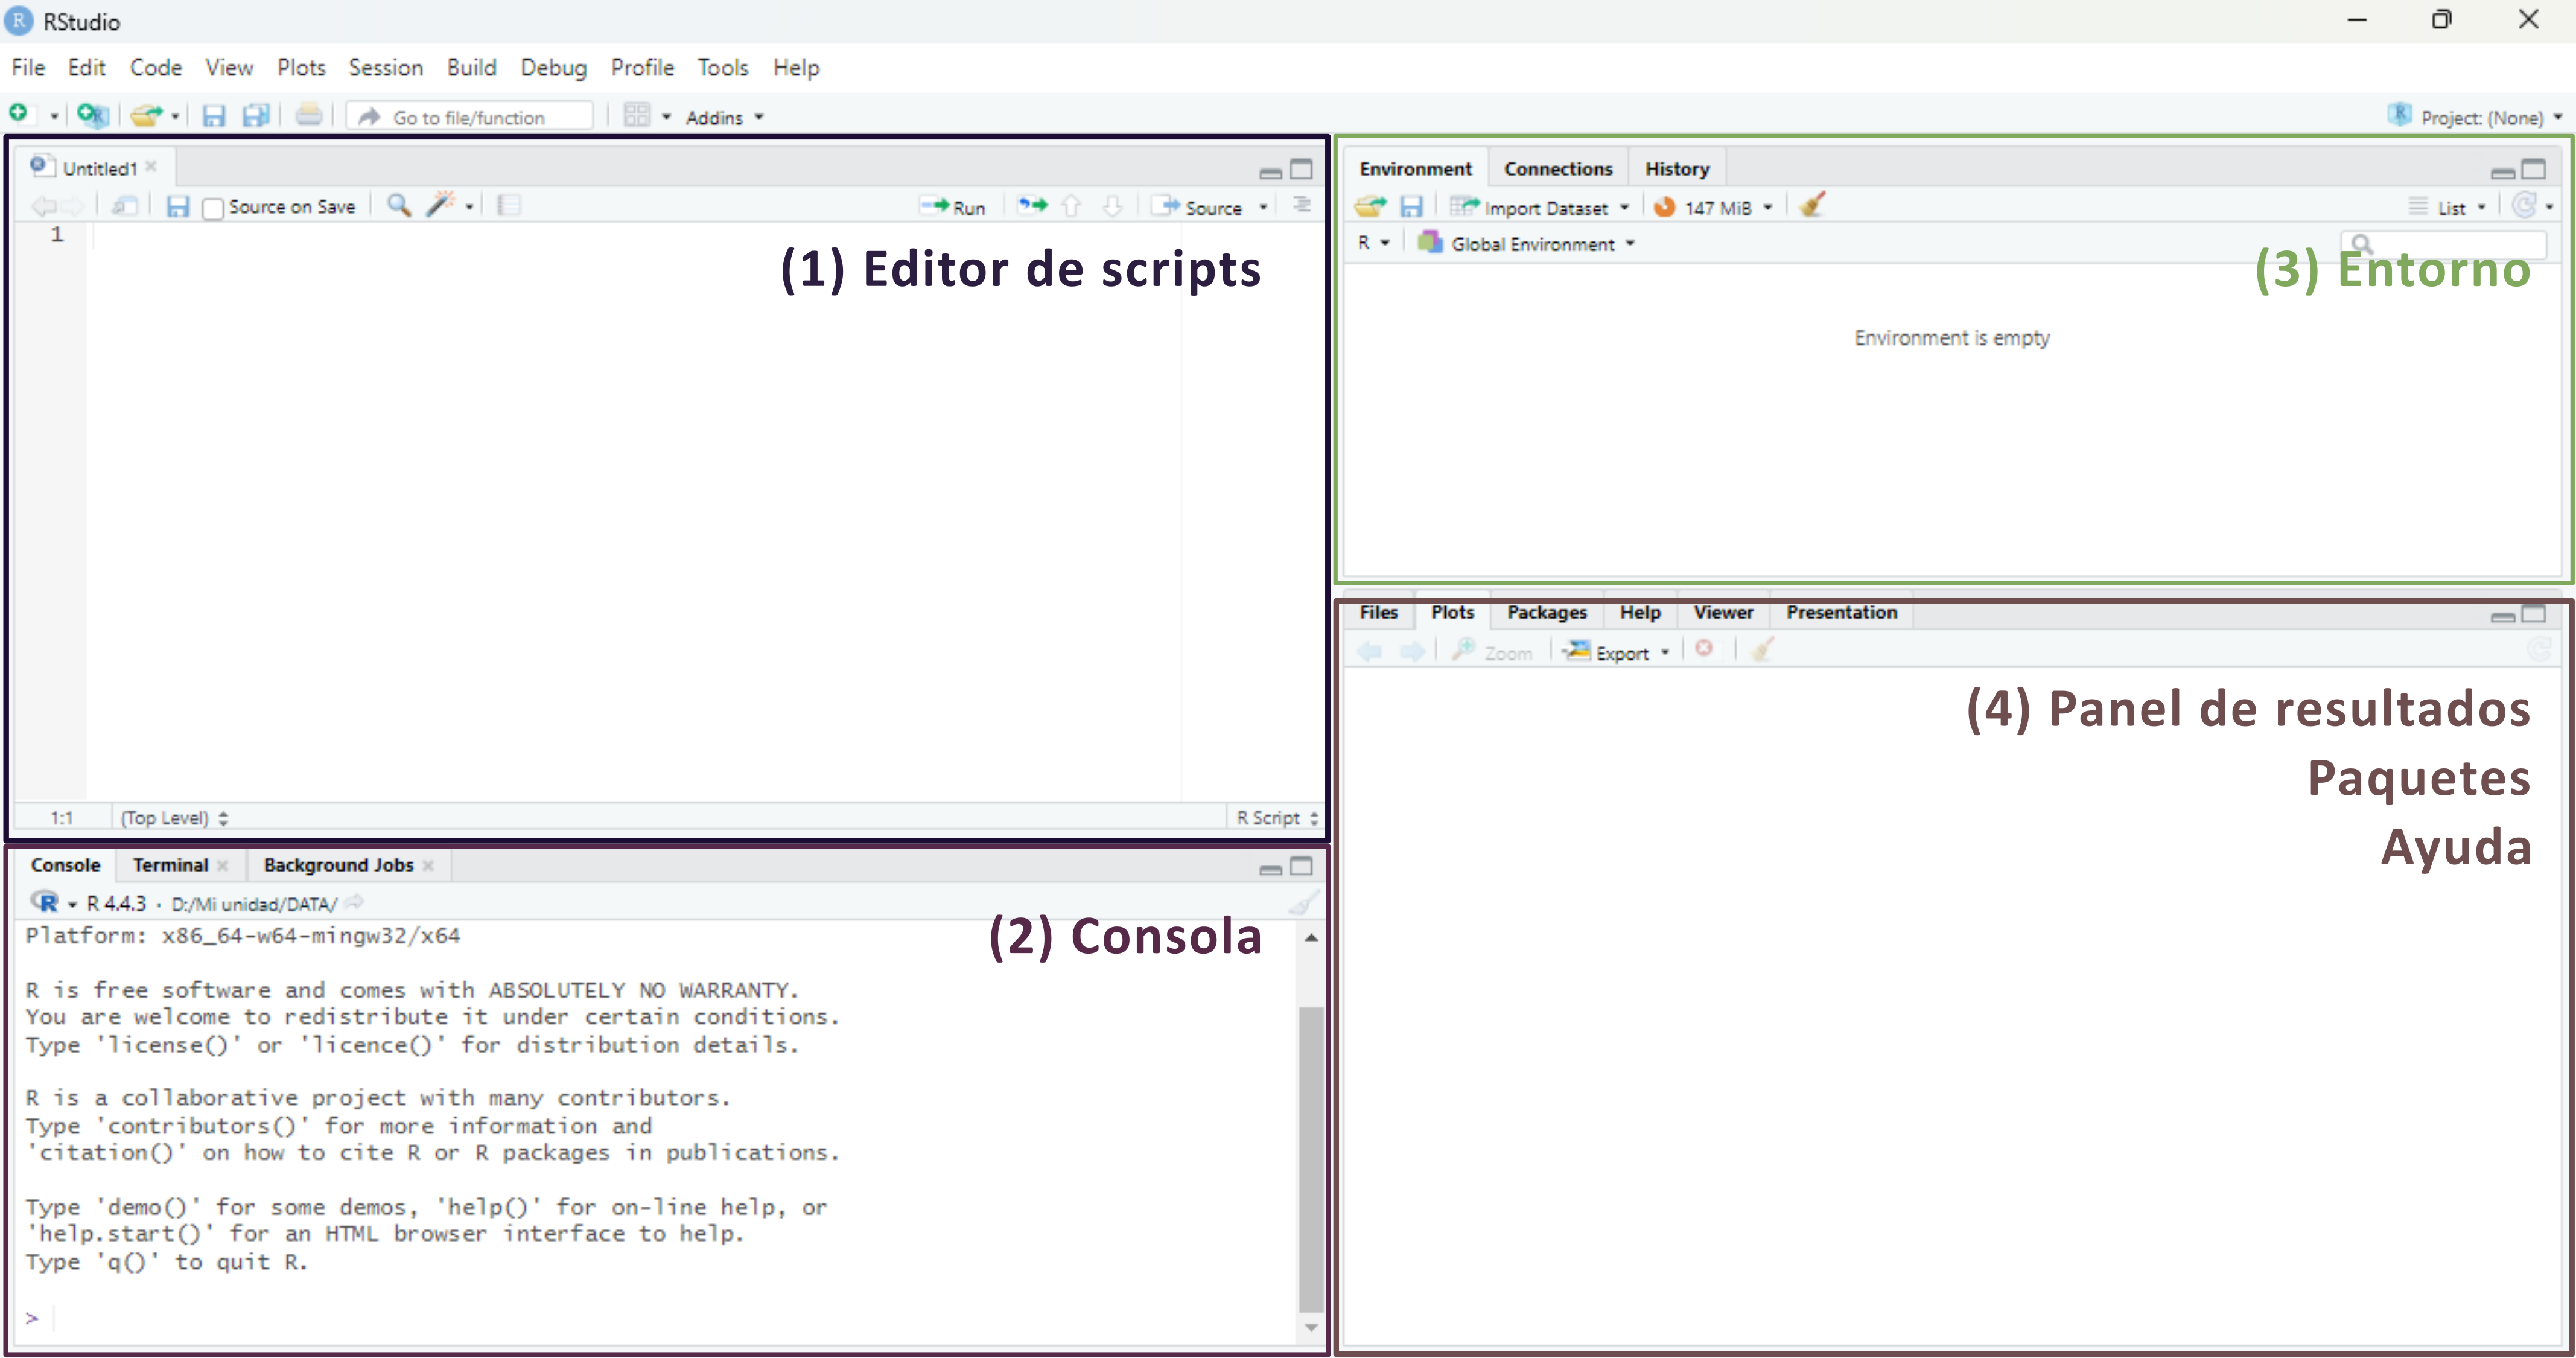
\includegraphics[width=0.95\linewidth,height=\textheight,keepaspectratio]{unidad_1/images/rstudio.png}
\end{center}

\begin{enumerate}
\def\labelenumi{\arabic{enumi}.}
\item
  \textbf{Editor de scripts} (\emph{Source}): permite crear y editar
  scripts de R, así como documentos R Markdown o Quarto.
\item
  \textbf{Consola de R} (\emph{Console}): muestra la salida del código
  ejecutado y ejecuta código de R de forma inmediata.
\item
  \textbf{Entorno} (\emph{Environment}): muestra los objetos creados
  durante la sesión, como vectores, \emph{dataframes} o funciones.
\item
  \textbf{Panel de resultados} (\emph{Output}): presenta los gráficos,
  tablas, visualizaciones en HTML y también incluye un explorador de
  archivos, visor de paquetes instalados y panel de ayuda.
\end{enumerate}

Para garantizar la reproducibilidad de los resultados, es recomendable
evitar el guardado automático del historial de objetos entre sesiones,
ya que puede generar confusión. Para desactivar esta opción, ir a
\texttt{Tools\ \textgreater{}\ Global\ Options} y desmarcar las casillas
de las opciones \textbf{Workspace} y \textbf{History} como se muestra en
la siguiente imagen:

\begin{center}
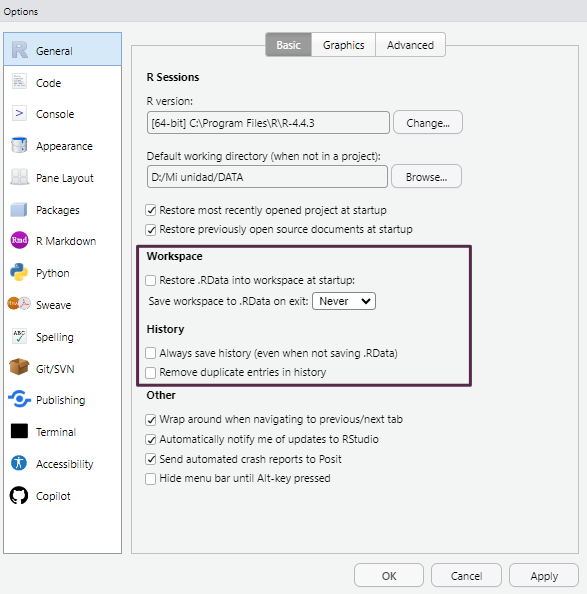
\includegraphics[width=6.25in,height=\textheight,keepaspectratio]{unidad_1/images/global_opts.png}
\end{center}

\section{Proyectos de RStudio}\label{proyectos-de-rstudio}

Los proyectos de RStudio permiten organizar de forma estructurada todo
el material asociado a un análisis: scripts, informes, bases de datos,
imágenes, etc. Cada proyecto se vincula a una carpeta específica del
sistema de archivos, y RStudio la utiliza como directorio de trabajo por
defecto. Esta carpeta puede estar ubicada en cualquier parte del sistema
de almacenamiento que deseemos (disco rígido, pendrive, disco externo,
etc).

Trabajar con proyectos facilita la importación de datos y evita errores
relacionados con rutas relativas o absolutas.

\subsection{Crear un proyecto}\label{crear-un-proyecto}

Para crear un nuevo proyecto, se puede utilizar el menú
\texttt{File\ \textgreater{}\ New\ Project...}. También accedemos a
generar un proyecto nuevo a partir de pulsar el acceso directo
\texttt{New\ Project...} ubicado en la esquina superior derecha de la
interfaz:

\begin{center}
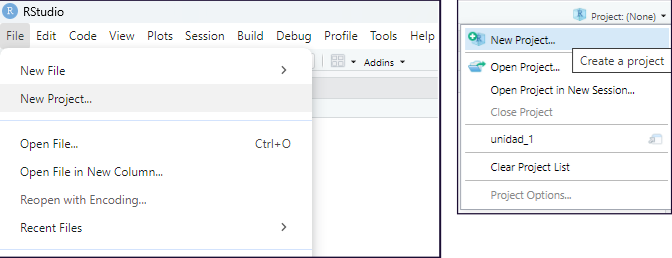
\includegraphics[width=6.25in,height=\textheight,keepaspectratio]{unidad_1/images/proyecto01.png}
\end{center}

En cualquiera de los dos casos aparecerá un cuadro de diálogo que
presenta tres opciones para crear el \textbf{nuevo proyecto} de RStudio:

\begin{center}
\pandocbounded{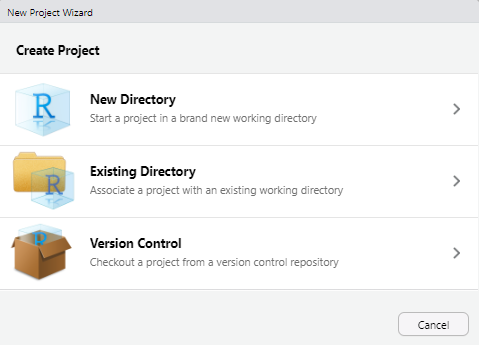
\includegraphics[keepaspectratio]{unidad_1/images/proyecto02.png}}
\end{center}

\begin{itemize}
\item
  \textbf{New Directory}: crea una nueva carpeta para el proyecto a la
  que deberemos asignarle un nombre, es la opción más habitual. Todos
  los archivos de configuración aparecerán asociados a esta nueva
  carpeta.
\item
  \textbf{Existing Directory}: vincula el proyecto a una \emph{carpeta
  ya existente} que contenga archivos previos con los que deseamos
  trabajar.
\item
  \textbf{Version Control}: permite clonar un repositorio (Git o SVN).
  Esta opción no se utilizará durante el curso.
\end{itemize}

Una vez que creamos un nuevo proyecto con la opción \textbf{New
Directory}, aparecerá una pantalla con una lista de tipos de proyectos
que se pueden crear en RStudio:

\begin{center}
\pandocbounded{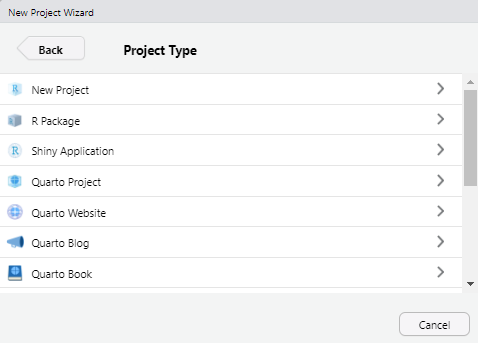
\includegraphics[keepaspectratio]{unidad_1/images/proyecto03.png}}
\end{center}

Durante este curso utilizaremos siempre la \textbf{primera opción}
(\textbf{New Project}). Las demás opciones están pensadas para usos más
específicos, como el desarrollo de paquetes de R, sitios web o
documentos con Quarto o R Markdown.

Al seleccionar \textbf{New Project}, se abrirá una nueva ventana con los
siguientes campos:

\begin{itemize}
\item
  \textbf{Directory name:} aquí debemos escribir el nombre del nuevo
  directorio (carpeta) que también será el nombre del proyecto. Por
  ejemplo, podemos llamarlo \texttt{Practicas\_R}.
\item
  \textbf{Create project as subdirectory of:} este campo permite definir
  en qué ubicación del sistema de archivos se guardará el proyecto.
  Podemos hacer clic en el botón \textbf{Browse\ldots{}} para abrir el
  explorador de archivos y seleccionar la carpeta contenedora. En
  nuestro ejemplo, lo ubicaremos dentro de \textbf{Mis Documentos}.
\end{itemize}

\begin{center}
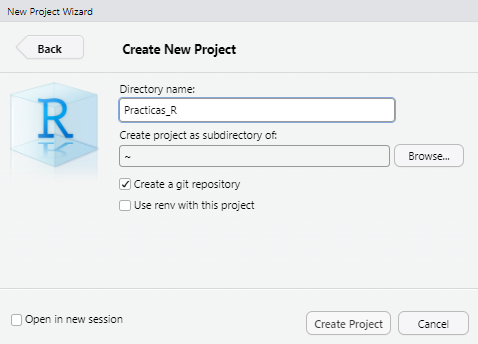
\includegraphics[width=4.98958in,height=\textheight,keepaspectratio]{unidad_1/images/proyecto04.png}
\end{center}

Una vez completados estos campos, hacemos clic en \textbf{Create
Project}.

Los proyectos en RStudio tienen entornos independientes, lo que
significa que si cerramos un proyecto o cambiamos a otro, la
configuración de cada uno se mantendrá inalterable sin interferir con
los demás.

Esto incluye los scripts abiertos, el directorio de trabajo, las
pestañas que dejamos activas y otros elementos del entorno que puedan
ser necesarios para continuar con un análisis. Este sistema permite
mantener organizados los distintos trabajos que llevamos adelante.

Echemos un vistazo a lo que RStudio realizó:

\begin{itemize}
\item
  En primer lugar el panel \textbf{Files} (pantalla inferior derecha)
  apunta a la nueva carpeta \textbf{Practicas\_R} y dentro de ella vemos
  un nuevo archivo el nombre del proyecto y la extensión
  \texttt{.Rproj}. Este archivo contiene todas las configuraciones para
  su proyecto.
\item
  El otro cambio se observa en la parte superior derecha, que muestra el
  nombre del proyecto. Si hacemos click en él, se desplegará el menú de
  proyectos. Desde aquí se puede abrir y cerrar proyectos, navegar
  rápidamente a proyectos que se han abierto recientemente y configurar
  las opciones de RStudio para cada uno de ellos.
\end{itemize}

\begin{center}
\pandocbounded{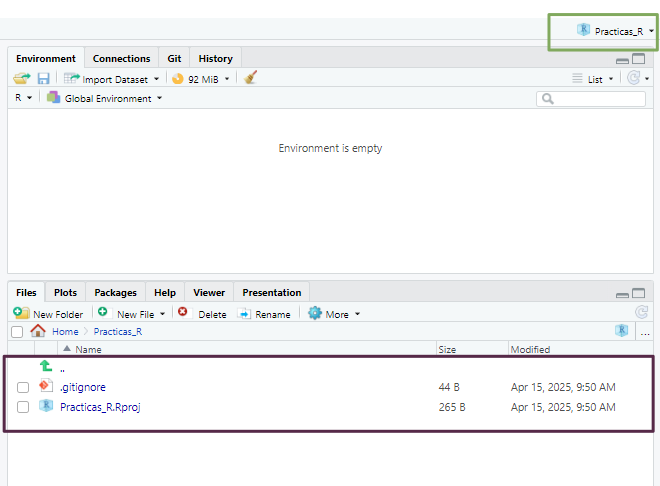
\includegraphics[keepaspectratio]{unidad_1/images/proyecto05.png}}
\end{center}

\subsection{Abrir un proyecto
existente}\label{abrir-un-proyecto-existente}

Cuando el proyecto ya existe, sea porque lo creamos nosotros o porque
alguien nos pasó una carpeta con un proyecto de RStudio creado vamos a
visualizar dentro de esa carpeta un archivo con extensión
\texttt{.Rproj}.

La forma más veloz para abrir el proyecto es ejecutar este archivo
(debería abrir una sesión de RStudio con el proyecto activo). La otra
forma es desde el menú superior derecho de RStudio en la opción
\textbf{Open project\ldots{}} y luego buscando en nuestro directorio el
mismo archivo \texttt{.Rproj}.

\begin{tcolorbox}[enhanced jigsaw, arc=.35mm, bottomrule=.15mm, breakable, colback=white, colframe=quarto-callout-warning-color-frame, left=2mm, leftrule=.75mm, opacityback=0, rightrule=.15mm, toprule=.15mm]

\vspace{-3mm}\textbf{Nota}\vspace{3mm}

El menú de proyectos del área superior derecha va guardando como
elementos recientes los proyectos que se van abriendo y también es una
forma rápida de acceder a ellos pulsando sobre estos atajos.

\end{tcolorbox}

\section{Scripts en RStudio}\label{scripts-en-rstudio}

Como vimos \hyperref[scripts-de-r]{\textbf{anteriormente}}, un script es
un archivo de código que contiene una secuencia de instrucciones
escritas en R. Estos scripts pueden ser reutilizados, modificados y
compartidos, lo que los convierte en una herramienta fundamental para
garantizar la reproducibilidad del trabajo.

\subsection{Crear un nuevo script}\label{crear-un-nuevo-script}

Tenemos varias formas de crear un script nuevo:

\begin{itemize}
\item
  Desde el menú superior:
  \texttt{File\ \textgreater{}\ New\ File\ \textgreater{}\ R\ Script}
\item
  Con el atajo de teclado: \texttt{Ctrl\ +\ Shift\ +\ N}
\item
  Desde la barra de herramientas: presionando el ícono
  \pandocbounded{
\includegraphics[keepaspectratio]{unidad_1/images/script_new.png}}
\end{itemize}

\subsection{Ejecutar scripts}\label{ejecutar-scripts}

La forma habitual de ejecutar el contenido de un script es línea por
línea, usando alguna de las siguientes opciones:

\begin{itemize}
\item
  Presionando el botón
  \pandocbounded{
\includegraphics[keepaspectratio]{unidad_1/images/script_run.png}}
  del editor de código de RStudio
\item
  Mediante el atajo de teclado \texttt{Ctrl\ +\ Enter}
\end{itemize}

Para ejecutar una línea, simplemente ubicamos el cursor en cualquier
parte de ella y presionamos el comando correspondiente. Luego de
ejecutarse, el cursor avanzará automáticamente a la siguiente línea de
código.

Mientras ejecutamos cada línea debemos ir observando la salida en la
consola (panel inferior izquierdo) y también los cambios que se dan en
el panel \emph{Environment} (panel superior derecho) donde aparecerán
los objetos que vayamos creando y manipulando.

\subsection{Edición de scripts}\label{ediciuxf3n-de-scripts}

Modificar o agregar líneas al script puede hacerse directamente en el
editor. Cada vez que realizamos un cambio, es necesario \textbf{volver a
ejecutar la línea} o bloque modificado para que los cambios se reflejen
en el entorno de trabajo.

Podemos probar y modificar tantas veces como sea necesario. Sin embargo,
debemos tener presente que cada manipulación en los objetos se mantiene
hasta que se vuelvan a cambiar y a veces, cuando los objetos están
vinculados con otras líneas de código posteriores tenemos que tener
cuidado que se mantenga la consistencia del script.

Por ejemplo: si definimos un vector numérico para realizar cálculos
matemáticos, pero luego lo sobrescribimos con un valor de tipo caracter,
los cálculos posteriores producirán un error y RStudio nos informará de
esto en la consola.

Por eso, es clave observar el contenido de los objetos en el panel
\textbf{Environment}, lo que nos ayuda a evitar errores y operaciones
incoherentes.

\subsection{Guardado de scripts}\label{guardado-de-scripts}

Cualquier agregado o modificación que hayamos realizado al script y nos
interese mantener nos obligará a guardar el archivo de código editado.

Existen distintas formas de guardar un script:

\begin{itemize}
\item
  Desde el menú superior: \texttt{File\ \textgreater{}\ Save}
\item
  Con el atajo de teclado: \texttt{Ctrl\ +\ S}
\item
  Presionando el ícono del disquete azul 💾
\end{itemize}

Si en cambio quisiera guardarlo como otro archivo para mantener el
script original, podemos guardarlo con diferente nombre o en otra
ubicación mediante \texttt{File\ \textgreater{}\ Save\ As...}

\subsection{Abrir scripts existentes}\label{abrir-scripts-existentes}

Los scripts que construyamos o nos compartan siempre tendrán extensión
\texttt{.R} y, por lo general, se encontrarán dentro de un proyecto.

Para abrir estos archivos \texttt{.R} podemos:

\begin{itemize}
\item
  Desde el menú superior: \texttt{File\ \textgreater{}\ Open\ file...}
\item
  Con el atajo de teclado: \texttt{Ctrl\ +\ O}
\item
  Haciendo click sobre el archivo desde el panel \emph{Files}
\item
  Presionando el botón de la carpeta amarilla 📂
\end{itemize}

Esto abrirá el script en una nueva pestaña dentro del editor de código.

\subsection{¿Cómo trabajaremos en este
curso?}\label{cuxf3mo-trabajaremos-en-este-curso}

En general, utilizaremos scripts dentro de \textbf{proyectos de
RStudio}. La secuencia recomendada será:

\begin{enumerate}
\def\labelenumi{\arabic{enumi}.}
\item
  \textbf{Descargar} desde el Aula Virtual un archivo comprimido
  conteniendo la carpeta, el proyecto, los scripts y archivos de datos.
\item
  \textbf{Descomprimir} el archivo en la ubicación que deseamos
  (recomendamos crear una carpeta destinada al curso).
\item
  Abrir la carpeta y ejecutar el archivo de proyecto \texttt{.Rproj}.
\item
  Una vez abierto RStudio con el proyecto activo, ubicamos los scripts
  desde el panel \textbf{Files}.
\item
  \textbf{Ejecutar} cada línea del script, leyendo la documentación del
  código y observando la salida en la consola y los cambios en el
  entorno
\end{enumerate}

\section{Herramientas de RStudio}\label{herramientas-de-rstudio}

Algunas de las herramientas fundamentales de RStudio son el asistente de
código, la ayuda en línea y el historial de comandos.

\subsection{Asistente de código}\label{asistente-de-cuxf3digo}

Al escribir en el editor o la consola, la tecla \texttt{Tab} activa el
autocompletado de funciones, nombres de objetos y argumentos, agilizando
la escritura y reduciendo errores de sintaxis. En versiones recientes,
el asistente también permite la previsualización de colores en los
gráficos, resaltar los paréntesis de cierre en funciones anidadas con
distintos colores y gestionar automáticamente la indentación del código.

\begin{center}
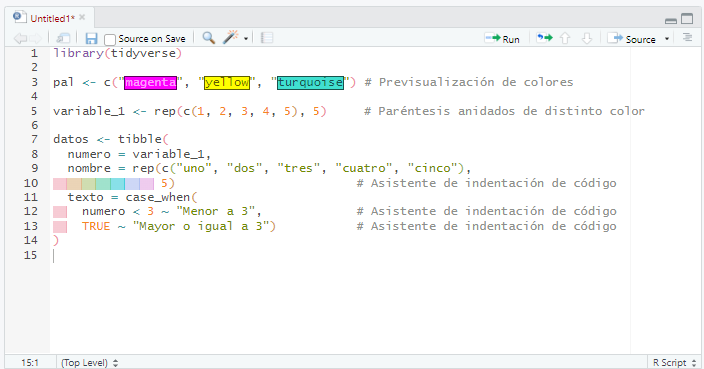
\includegraphics[width=6.25in,height=\textheight,keepaspectratio]{unidad_1/images/asistente.png}
\end{center}

Muchas de estas opciones se pueden configurar desde el menú
\texttt{Code} y desde
\texttt{Tools\ \textgreater{}\ Global\ Options\ \textgreater{}\ Code}(pestañas
\textbf{Editing} y \textbf{Display}).

\begin{center}
\pandocbounded{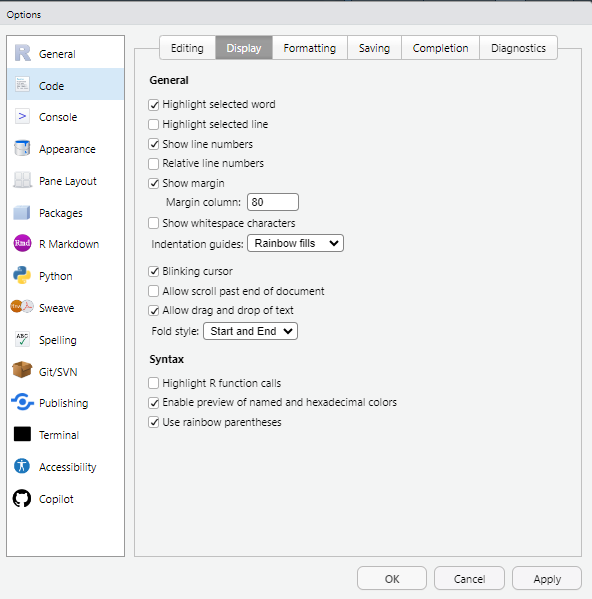
\includegraphics[keepaspectratio]{unidad_1/images/code_display.png}}
\end{center}

\subsection{Ayuda en línea}\label{ayuda-en-luxednea}

Al posicionar el cursor sobre el nombre de una función en el editor y
presionar \texttt{F1}, se accede directamente a la documentación
correspondiente en el panel \textbf{Help} (habitualmente ubicado en la
esquina inferior derecha).

\begin{center}
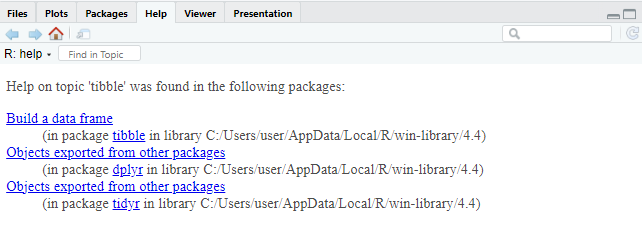
\includegraphics[width=6.25in,height=\textheight,keepaspectratio]{unidad_1/images/help.png}
\end{center}

\subsection{Historial de comandos}\label{historial-de-comandos}

En la consola, al usar las teclas de flecha arriba/abajo, se puede
navegar por los comandos ejecutados durante la sesión actual. Además, el
panel \textbf{History} (parte superior derecha) almacena los comandos de
todas las sesiones previas, permitiendo reutilizarlos con un clic en
\textbf{To Console} (\texttt{Enter}) o \textbf{To Source}
(\texttt{Shift\ +\ Enter}), según se desee insertarlos en la consola o
en el script activo.

\begin{center}
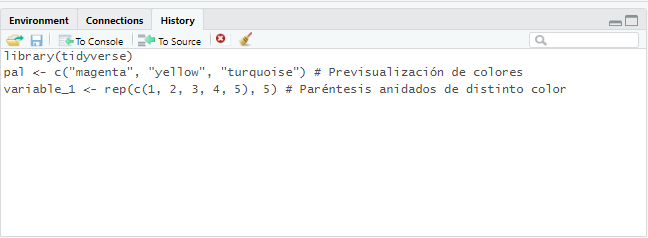
\includegraphics[width=6.25in,height=\textheight,keepaspectratio]{unidad_1/images/historial.png}
\end{center}

\section{Atajos de teclado (Windows)}\label{atajos-de-teclado-windows}

\begin{table}
\centering
\begin{tabular}[t]{l|l}
\hline
\cellcolor[HTML]{2f2e4e}{\textcolor{white}{Menú}} & \cellcolor[HTML]{2f2e4e}{\textcolor{white}{Descripción}}\\
\hline
Archivo (File) & \\
\hline
Ctrl + Shift + N & Crea un nuevo script\\
\hline
Ctrl + O & Abre un script guardado\\
\hline
Ctrl + S & Guarda el script activo\\
\hline
Ctrl + W & Cierra el script activo\\
\hline
Ctrl + Q & Sale del programa RStudio\\
\hline
Edición (Edit) & \\
\hline
Ctrl + F & Abre la ventana de búsqueda (para buscar palabras dentro de un script)\\
\hline
Ctrl + L & Limpia la consola\\
\hline
Código (Code) & \\
\hline
Ctrl + Enter & Ejecuta la línea de código donde está situado el cursor\\
\hline
Ctrl + Alt + R & Ejecuta todo el código del script activo\\
\hline
Ctrl + Shift + N & Inserta nueva sección de código\\
\hline
Ctrl + Shift + R & Inserta nueva sección de comentarios de texto\\
\hline
Sesión (Session) & \\
\hline
Ctrl + Shift + H & Abre la ventana para establecer directorio de trabajo\\
\hline
Ctrl + Shift + F10 & Reinicia la sesión de R\\
\hline
Herramientas (Tools) & \\
\hline
Alt + Shift + K & Abre la lista de ayuda de atajos de teclado\\
\hline
\end{tabular}
\end{table}

\section{Paquetes}\label{paquetes}

Existen dos formas principales de descargar paquetes: directamente desde
RStudio o desde el
\href{https://cran.r-project.org/web/packages/}{\textbf{sitio web de
CRAN}}, descargándolos como archivos comprimidos. Si el equipo cuenta
con conexión a Internet, lo más práctico es realizar la descarga
directamente desde RStudio. En cambio, si no se dispone de acceso
permanente a la red, es posible descargar los paquetes desde otro equipo
y luego transferirlos como archivos \texttt{.zip} o \texttt{.tar.gz} al
equipo donde se encuentra instalado R.

Cuando accedemos al sitio web de CRAN y buscamos un paquete específico,
encontraremos información útil como una breve descripción del paquete,
el número de versión, la fecha de publicación, el nombre del autor,
documentación asociada y enlaces de descarga específicos para cada
sistema operativo.

Dado que la mayoría de las computadoras hoy en día cuentan con acceso a
Internet, en este curso nos enfocaremos en la instalación y activación
de paquetes directamente desde RStudio.

Dentro del entorno de RStudio, la gestión de paquetes se realiza desde
la pestaña \emph{Packages}, ubicada en el panel inferior derecho. Esta
interfaz facilita tareas como la instalación, actualización y activación
de paquetes, y cada acción que realizamos desde la interfaz gráfica se
traduce internamente en la ejecución de funciones del lenguaje R que
pueden observarse en la consola.

Para instalar un paquete nuevo, simplemente pulsamos el botón
\emph{Install} dentro de la pestaña \emph{Packages}, lo cual abrirá una
ventana emergente.

\begin{center}
\pandocbounded{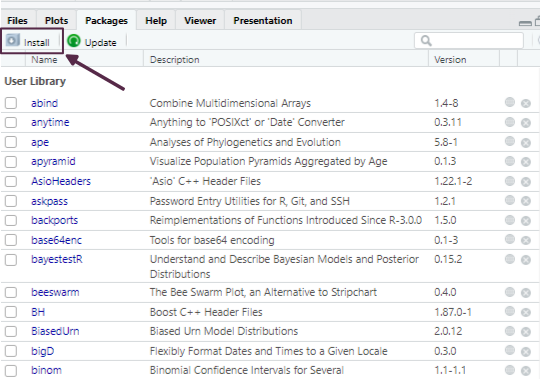
\includegraphics[keepaspectratio]{unidad_1/images/rstudio_paquetes01.png}}
\end{center}

Allí podemos escribir el nombre del paquete que deseamos instalar. Para
asegurarnos de que también se descarguen e instalen automáticamente los
paquetes de los que depende, es importante tildar la opción
\emph{Install dependencies}.

\begin{center}
\pandocbounded{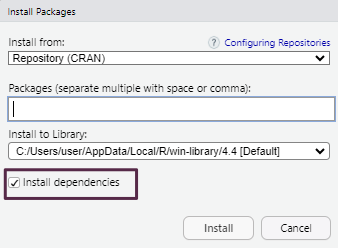
\includegraphics[keepaspectratio]{unidad_1/images/rstudio_paquetes02.png}}
\end{center}

Como alternativa, también podemos realizar la instalación desde el
editor de scripts mediante el siguiente comando:

\begin{Shaded}
\begin{Highlighting}[]
\FunctionTok{install.packages}\NormalTok{(}\StringTok{"nombre\_del\_paquete"}\NormalTok{, }\AttributeTok{dependencies =} \ConstantTok{TRUE}\NormalTok{)}
\end{Highlighting}
\end{Shaded}

\begin{tcolorbox}[enhanced jigsaw, arc=.35mm, bottomrule=.15mm, breakable, colback=white, colframe=quarto-callout-note-color-frame, left=2mm, leftrule=.75mm, opacityback=0, rightrule=.15mm, toprule=.15mm]

Para facilitar la instalación de los paquetes requeridos durante el
curso, recomendamos descargar el archivo
\textbf{``\href{../files/datos_y_paquetes.zip}{Paquetes y datos para el
curso}''}, descomprimirlo y ejecutar el script que se encuentra en su
interior.

\end{tcolorbox}

\section{Lectura de archivos de
datos}\label{lectura-de-archivos-de-datos}

R permite importar tablas de datos desde diversos formatos, tanto
utilizando funciones de \textbf{R base} como funciones provistas por
paquetes específicos.

El formato más común es el \textbf{texto plano} (ASCII), donde los
valores están organizados en columnas separadas por caracteres
delimitadores. Los separadores más habituales incluyen:

\begin{itemize}
\item
  Coma (\texttt{,})
\item
  Punto y coma (\texttt{;})
\item
  Tabulación (\texttt{\textbackslash{}t})
\item
  Barra vertical (\texttt{\textbar{}})
\end{itemize}

Estos archivos suelen tener una \textbf{cabecera} (\emph{header}) en la
primera fila con los nombres de las variables, y cada columna debe
contener datos del mismo tipo (números, texto, lógicos, etc.).

Para importar correctamente un archivo es importante conocer su
estructura:

\begin{itemize}
\item
  Si incluye o no cabecera.
\item
  Qué carácter se usa como separador.
\item
  El tipo de codificación (UTF-8, Latin1, etc.).
\end{itemize}

Dado que son archivos de texto, pueden visualizarse con editores simples
como el Bloc de Notas o desde RStudio, lo que facilita su inspección
previa.

Para cargar los datos desde un archivo de texto plano usamos el código:

\begin{Shaded}
\begin{Highlighting}[]
\NormalTok{datos }\OtherTok{\textless{}{-}} \FunctionTok{read.xxx}\NormalTok{(}\StringTok{"mis\_datos.xxx"}\NormalTok{)}
\end{Highlighting}
\end{Shaded}

(Se debe reemplazar \texttt{read.xxx()} por la función correspondiente:
\texttt{read.table()}, \texttt{read.csv()}, \texttt{read\_delim()},
\texttt{read\_excel()}, etc., según la extensión del archivo).

R también permite cargar bases de datos incluidas en paquetes instalados
mediante:

\begin{Shaded}
\begin{Highlighting}[]
\FunctionTok{data}\NormalTok{(nombre\_datos)}

\NormalTok{datos }\OtherTok{\textless{}{-}}\NormalTok{ nombre\_datos}
\end{Highlighting}
\end{Shaded}

\section{Buenas prácticas}\label{buenas-pruxe1cticas}

Adoptar buenas prácticas desde el inicio mejora la reproducibilidad,
facilita el trabajo colaborativo y reduce errores. Algunas
recomendaciones clave son:

\begin{itemize}
\item
  Trabajar \textbf{siempre} dentro de un \textbf{proyecto de RStudio}
  (\texttt{.Rproj}). Esto permite organizar los archivos, mantener rutas
  relativas consistentes y acceder a funcionalidades específicas como
  control de versiones o panel de archivos integrados.
\item
  Incluir al comienzo de cada script las líneas de \textbf{activación de
  paquetes} necesarios, utilizando la función \texttt{library()}.
\item
  \textbf{Cargar los datos} una vez activados los paquetes, para
  garantizar que todas las funciones requeridas estén disponibles.
\item
  Documentar el código mediante \textbf{comentarios} iniciados con
  \texttt{\#}. Esto permite entender qué hace cada bloque de código,
  facilitando futuras modificaciones o revisiones.
\item
  \textbf{Usar espacios e indentación adecuada} para mejorar la
  legibilidad. Esto es especialmente importante en estructuras anidadas
  (como condicionales, bucles o funciones).
\end{itemize}

\chapter{Introducción a tidyverse}\label{introducciuxf3n-a-tidyverse}

\begin{center}

\includegraphics[width=0.44\linewidth,height=\textheight,keepaspectratio]{unidad_1/images/tidyverse.png}
\end{center}

\section{Introducción}\label{introducciuxf3n}

\emph{Tidyverse} {[}@tidyverse{]} es el nombre que recibe el conjunto de
paquetes desarrollados y/o promovidos por
\href{https://en.wikipedia.org/wiki/Hadley_Wickham}{\textbf{Hadley
Wickham}} (jefe científico en Posit/RStudio) y su equipo, orientado al
trabajo de ciencia de datos con R. Estos paquetes están diseñados para
integrarse de manera coherente, compartiendo una misma filosofía de
diseño conocida como
\href{https://cran.r-project.org/web/packages/tidyverse/vignettes/manifesto.html}{\textbf{\emph{The
tidy tools manifesto}}}.

Los cuatro principios básicos sobre los que se construye
\emph{tidyverse} son:

\begin{itemize}
\item
  Reutilización de estructuras de datos
\item
  Resolución de problemas complejos combinando varias piezas sencillas
\item
  Uso de programación funcional
\item
  Diseño orientado a las personas
\end{itemize}

Los paquetes incluidos cubren todas las etapas del análisis de datos
dentro de R: importación y ordenamiento de los datos (\emph{tidy data}),
transformación, visualización, modelado y la posterior comunicación de
resultados.

La palabra \emph{tidy} se traduce como ``ordenado'', y hace referencia a
una estructura específica que deben cumplir los datos:

\begin{itemize}
\tightlist
\item
  Cada \textbf{\emph{variable}} es una \emph{columna} de la tabla de
  datos.
\item
  Cada \textbf{\emph{observación}} es una \emph{fila} de la tabla de
  datos.
\item
  Cada \textbf{\emph{tabla}} responde a una \emph{unidad de observación
  o} análisis.
\end{itemize}

\begin{center}
\pandocbounded{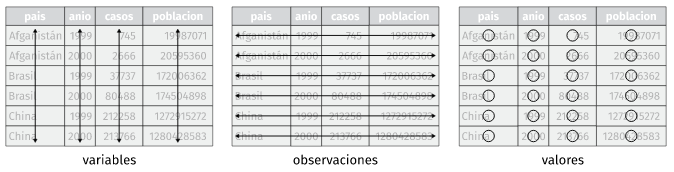
\includegraphics[keepaspectratio]{unidad_1/images/tidy.PNG}}
\end{center}

Además de los paquetes principales, al instalar \texttt{tidyverse} se
incluyen otros que permiten trabajar con fechas, cadenas de caracteres o
factores, también siguiendo los mismos principios.

Uno de los objetivos de los desarrolladores fue dotar a la sintaxis de
estos paquetes de una \textbf{gramática} clara: funciones cuyos nombres
y argumentos permiten construir ``\emph{frases}'' que sean
semánticamente comprensibles. Un ejemplo de esto se ve en el paquete
\texttt{dplyr}, donde la mayoría de las funciones son verbos en inglés
como \texttt{filter()}, \texttt{mutate()}, \texttt{summarise()}, lo que
facilita su lectura y comprensión.

El paquete \texttt{tidyverse} (versión 2.0.0) puede instalarse desde el
repositorio oficial CRAN mediante el menú \emph{Packages} de RStudio, o
ejecutando el siguiente código:

\begin{Shaded}
\begin{Highlighting}[]
\FunctionTok{install.packages}\NormalTok{(}\StringTok{"tidyverse"}\NormalTok{)}
\end{Highlighting}
\end{Shaded}

Una vez instalado, se activa mediante:

\begin{Shaded}
\begin{Highlighting}[]
\FunctionTok{library}\NormalTok{(tidyverse)}
\end{Highlighting}
\end{Shaded}

Al activarlo, se muestra un mensaje con la versión instalada, la lista
de paquetes que se cargan automáticamente y posibles conflictos de
nombres entre funciones. Esto es habitual cuando se utilizan múltiples
paquetes, ya que algunas funciones pueden llamarse igual. Por ejemplo,
la función \texttt{filter()} existe tanto en el paquete \texttt{stats}
como en \texttt{dplyr}. Al cargar \texttt{tidyverse}, R avisa de esta
superposición:

\texttt{✖️dplyr::filter()\ masks\ stats::filter()}

Cuando necesitamos asegurarnos de que estamos usando la función de un
paquete específico, se recomienda usar la notación \texttt{::}, por
ejemplo:

\begin{Shaded}
\begin{Highlighting}[]
\CommentTok{\# Función filter() del paquete stats}
\NormalTok{stats}\SpecialCharTok{::}\FunctionTok{filter}\NormalTok{()}

\CommentTok{\# Función filter() del paquete tidyverse}
\NormalTok{dplyr}\SpecialCharTok{::}\FunctionTok{filter}\NormalTok{()}
\end{Highlighting}
\end{Shaded}

Una estrategia útil cuando trabajamos con varios paquetes es cargar
\texttt{tidyverse} al final de la lista de paquetes, para que sus
funciones sobrescriban las de otros paquetes si fuese necesario:

\begin{Shaded}
\begin{Highlighting}[]
\FunctionTok{library}\NormalTok{(stats)}
\FunctionTok{library}\NormalTok{(tidyverse)}
\end{Highlighting}
\end{Shaded}

Los paquetes que se instalan con la versión actual de \texttt{tidyverse}
pueden consultarse ejecutando:

\begin{Shaded}
\begin{Highlighting}[]
\FunctionTok{tidyverse\_packages}\NormalTok{()}
\end{Highlighting}
\end{Shaded}

\begin{verbatim}
 [1] "broom"         "conflicted"    "cli"           "dbplyr"       
 [5] "dplyr"         "dtplyr"        "forcats"       "ggplot2"      
 [9] "googledrive"   "googlesheets4" "haven"         "hms"          
[13] "httr"          "jsonlite"      "lubridate"     "magrittr"     
[17] "modelr"        "pillar"        "purrr"         "ragg"         
[21] "readr"         "readxl"        "reprex"        "rlang"        
[25] "rstudioapi"    "rvest"         "stringr"       "tibble"       
[29] "tidyr"         "xml2"          "tidyverse"    
\end{verbatim}

Además, existen muchos otros paquetes que siguen la misma filosofía pero
no están incluidos por defecto. En esos casos, deben instalarse y
activarse individualmente.

\begin{tcolorbox}[enhanced jigsaw, arc=.35mm, bottomrule=.15mm, breakable, colback=white, colframe=quarto-callout-warning-color-frame, left=2mm, leftrule=.75mm, opacityback=0, rightrule=.15mm, toprule=.15mm]
\begin{minipage}[t]{5.5mm}
\textcolor{quarto-callout-warning-color}{\faExclamationTriangle}
\end{minipage}%
\begin{minipage}[t]{\textwidth - 5.5mm}

Para profundizar el uso de \texttt{tidyverse}, se recomienda consultar
las siguientes fuentes:

\begin{itemize}
\item
  Sitio oficial:
  \href{https://www.tidyverse.org/}{\textbf{https://www.tidyverse.org/}}
\item
  Libro \emph{R para Ciencia de Datos:}
  \href{https://es.r4ds.hadley.nz/index.html}{\textbf{r4ds}} o la nueva
  versión \href{https://r4ds.hadley.nz/}{\textbf{\emph{r4ds 2e}}} (por
  ahora solo disponible en inglés).
\item
  \href{https://www.epirhandbook.com/es/index.es.html}{\textbf{EpiRhandbook
  en español}}
\end{itemize}

\end{minipage}%
\end{tcolorbox}

\section{\texorpdfstring{\emph{Dataframes} con
\texttt{tibble}}{Dataframes con tibble}}\label{dataframes-con-tibble}

\href{https://tibble.tidyverse.org/}{\begin{center}

\includegraphics[width=0.2\linewidth,height=\textheight,keepaspectratio]{unidad_1/images/tibble.png}
\end{center}
}

Uno de los paquetes que forman parte del núcleo básico de
\emph{tidyverse} es \texttt{tibble} {[}@tibble{]}, que introduce una
versión moderna del objeto \texttt{data.frame}. Todas las funciones que
generan tablas de datos en \emph{tidyverse} devuelven objetos
\emph{tibble} (\texttt{tbl\_df}), los cuales son más eficientes y
amigables para el flujo de trabajo.

Las principales ventajas de trabajar con \texttt{tibble} son:

\begin{itemize}
\item
  Impresión en consola más legible y controlada (muestran un número
  limitado de filas y columnas).
\item
  No cambian automáticamente el tipo de datos.
\item
  Permiten nombres de columnas con espacios o caracteres especiales si
  se encierran entre comillas invertidas \texttt{\textasciigrave{}}
  (aunque \textbf{no se recomienda}).
\end{itemize}

Para crear un objeto \emph{tibble} manualmente usamos el siguiente
código:

\begin{Shaded}
\begin{Highlighting}[]
\NormalTok{datos }\OtherTok{\textless{}{-}} \FunctionTok{tibble}\NormalTok{(}
  \AttributeTok{nombre =} \FunctionTok{c}\NormalTok{(}\StringTok{"Ana"}\NormalTok{, }\StringTok{"Luis"}\NormalTok{, }\StringTok{"María"}\NormalTok{),}
  \AttributeTok{edad =} \FunctionTok{c}\NormalTok{(}\DecValTok{34}\NormalTok{, }\DecValTok{28}\NormalTok{, }\DecValTok{45}\NormalTok{),}
  \AttributeTok{altura =} \FunctionTok{c}\NormalTok{(}\FloatTok{1.65}\NormalTok{, }\FloatTok{1.80}\NormalTok{, }\FloatTok{1.70}\NormalTok{)}
\NormalTok{)}
\end{Highlighting}
\end{Shaded}

\section{\texorpdfstring{Tuberías con
\texttt{magrittr}}{Tuberías con magrittr}}\label{tuberuxedas-con-magrittr}

\href{https://magrittr.tidyverse.org/}{\begin{center}

\includegraphics[width=0.2\linewidth,height=\textheight,keepaspectratio]{unidad_1/images/magrittr.png}
\end{center}
}

Una de las incorporaciones más útiles y transversales del ecosistema
\emph{tidyverse} es el uso de ``\emph{tuberías''} o \emph{pipe
operators}. Una tubería conecta un bloque de código con otro,
permitiendo encadenar operaciones de manera legible. El operador
\texttt{\%\textgreater{}\%}, proveniente del paquete \texttt{magrittr}
{[}@magrittr{]}, transforma llamadas de funciones anidadas (con
múltiples paréntesis) en una secuencia de pasos más simple de leer y
escribir.

A partir de la versión 4.1.0 de R, también se incorporó una
\textbf{tubería nativa} (\texttt{\textbar{}\textgreater{}}), con un
comportamiento muy similar. Ambas opciones son válidas y su uso es
prácticamente equivalente.

Este enfoque refleja el principio de que \emph{cada función representa
un paso en una secuencia lógica de transformación de datos}. La forma de
trabajar se puede ver en el siguiente esquema general:

\begin{center}
\pandocbounded{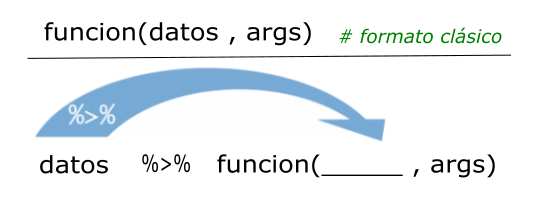
\includegraphics[keepaspectratio]{unidad_1/images/pipe.png}}
\end{center}

A continuación, mostramos un ejemplo comparativo de cómo cambia la
sintaxis usando el dataset incorporado en R \texttt{mtcars}, que
contiene datos sobre autos:

\begin{Shaded}
\begin{Highlighting}[]
\FunctionTok{head}\NormalTok{(}\FunctionTok{sqrt}\NormalTok{(mtcars))}
\end{Highlighting}
\end{Shaded}

\begin{verbatim}
                       mpg      cyl     disp        hp     drat       wt
Mazda RX4         4.582576 2.449490 12.64911 10.488088 1.974842 1.618641
Mazda RX4 Wag     4.582576 2.449490 12.64911 10.488088 1.974842 1.695582
Datsun 710        4.774935 2.000000 10.39230  9.643651 1.962142 1.523155
Hornet 4 Drive    4.626013 2.449490 16.06238 10.488088 1.754993 1.793042
Hornet Sportabout 4.324350 2.828427 18.97367 13.228757 1.774824 1.854724
Valiant           4.254409 2.449490 15.00000 10.246951 1.661325 1.860108
                      qsec vs am     gear     carb
Mazda RX4         4.057093  0  1 2.000000 2.000000
Mazda RX4 Wag     4.125530  0  1 2.000000 2.000000
Datsun 710        4.313931  1  1 2.000000 1.000000
Hornet 4 Drive    4.409082  1  0 1.732051 1.000000
Hornet Sportabout 4.125530  0  0 1.732051 1.414214
Valiant           4.496665  1  0 1.732051 1.000000
\end{verbatim}

En la línea de código anterior estamos pidiendo mostrar la cabecera (6
primeras observaciones de la tabla de datos) de la raíz cuadrada de los
valores de la tabla \texttt{mtcars}, en formato del lenguaje clásico
(anidado).

Ahora activamos \texttt{magrittr} y ejecutamos la línea anterior en
formato tubería:

\begin{Shaded}
\begin{Highlighting}[]
\CommentTok{\# Activa paquete}
\FunctionTok{library}\NormalTok{(magrittr)}

\CommentTok{\# Formato tubería}
\NormalTok{mtcars }\SpecialCharTok{\%\textgreater{}\%}
  \FunctionTok{sqrt}\NormalTok{() }\SpecialCharTok{\%\textgreater{}\%}
  \FunctionTok{head}\NormalTok{()}
\end{Highlighting}
\end{Shaded}

\begin{verbatim}
                       mpg      cyl     disp        hp     drat       wt
Mazda RX4         4.582576 2.449490 12.64911 10.488088 1.974842 1.618641
Mazda RX4 Wag     4.582576 2.449490 12.64911 10.488088 1.974842 1.695582
Datsun 710        4.774935 2.000000 10.39230  9.643651 1.962142 1.523155
Hornet 4 Drive    4.626013 2.449490 16.06238 10.488088 1.754993 1.793042
Hornet Sportabout 4.324350 2.828427 18.97367 13.228757 1.774824 1.854724
Valiant           4.254409 2.449490 15.00000 10.246951 1.661325 1.860108
                      qsec vs am     gear     carb
Mazda RX4         4.057093  0  1 2.000000 2.000000
Mazda RX4 Wag     4.125530  0  1 2.000000 2.000000
Datsun 710        4.313931  1  1 2.000000 1.000000
Hornet 4 Drive    4.409082  1  0 1.732051 1.000000
Hornet Sportabout 4.125530  0  0 1.732051 1.414214
Valiant           4.496665  1  0 1.732051 1.000000
\end{verbatim}

Podemos hacer lo mismo con la tubería nativa de R sin activar ningún
paquete (revisar que esté activada desde
\texttt{Tools\ \textgreater{}\ Global\ Options}):

\begin{Shaded}
\begin{Highlighting}[]
\CommentTok{\# Tubería nativa}
\NormalTok{mtcars }\SpecialCharTok{|\textgreater{}}
  \FunctionTok{sqrt}\NormalTok{() }\SpecialCharTok{|\textgreater{}}
  \FunctionTok{head}\NormalTok{()}
\end{Highlighting}
\end{Shaded}

\begin{verbatim}
                       mpg      cyl     disp        hp     drat       wt
Mazda RX4         4.582576 2.449490 12.64911 10.488088 1.974842 1.618641
Mazda RX4 Wag     4.582576 2.449490 12.64911 10.488088 1.974842 1.695582
Datsun 710        4.774935 2.000000 10.39230  9.643651 1.962142 1.523155
Hornet 4 Drive    4.626013 2.449490 16.06238 10.488088 1.754993 1.793042
Hornet Sportabout 4.324350 2.828427 18.97367 13.228757 1.774824 1.854724
Valiant           4.254409 2.449490 15.00000 10.246951 1.661325 1.860108
                      qsec vs am     gear     carb
Mazda RX4         4.057093  0  1 2.000000 2.000000
Mazda RX4 Wag     4.125530  0  1 2.000000 2.000000
Datsun 710        4.313931  1  1 2.000000 1.000000
Hornet 4 Drive    4.409082  1  0 1.732051 1.000000
Hornet Sportabout 4.125530  0  0 1.732051 1.414214
Valiant           4.496665  1  0 1.732051 1.000000
\end{verbatim}

Las tuberías le dan mucha mas claridad al código separándolo en partes,
como si fuesen oraciones de un párrafo.

\section{Lectura y escritura de
datos}\label{lectura-y-escritura-de-datos}

\subsection{\texorpdfstring{Archivos de texto plano con
\texttt{readr}}{Archivos de texto plano con readr}}\label{archivos-de-texto-plano-con-readr}

\href{https://readr.tidyverse.org/}{\begin{center}

\includegraphics[width=0.2\linewidth,height=\textheight,keepaspectratio]{unidad_1/images/readr.png}
\end{center}
}

El paquete \texttt{readr} {[}@readr{]} contiene funciones similares a
las de la familia \texttt{read.table()} de R base, pero desarrollados
bajo el ecosistema \texttt{tidyverse}.

Los archivos de texto plano (ASCII u otras codificaciones) son
universalmente utilizados por la mayoría de los gestores de bases de
datos y planillas de cálculo. Generalmente se encuentran con extensiones
\texttt{.txt} o \texttt{.csv} (por \emph{comma-separated values}) y son
el tipo de archivo de datos más habitual en R.

Estos datos planos tienen dos características principales:

\begin{itemize}
\tightlist
\item
  La cabecera (en inglés \emph{header}).
\item
  El carácter o símbolo separador que indica la separación de columnas:
  pueden estar separadas por comas, punto y coma, tabulación, etc.
\end{itemize}

La presencia o no de una cabecera se maneja con los argumentos
\texttt{col\_names} y \texttt{skip}:

\begin{itemize}
\item
  \texttt{col\_names\ =\ TRUE} indica que la primera fila contiene los
  nombres de las columnas (cabecera).
\item
  \texttt{col\_names\ =\ FALSE} indica que no hay cabecera y las
  columnas se nombran automáticamente (\texttt{X1}, \texttt{X2}, etc).
\item
  \texttt{skip\ =\ 0} (valor por defecto) lee los datos desde la primera
  fila, pero si hay encabezados complejos (por ejemplo, títulos y
  subtítulos ), se puede indicar cuántas filas deben omitirse. Ejemplo:
  \texttt{skip\ =\ 5} omite las primeras 5 filas del archivo.
\end{itemize}

Otro aspecto a considerar es el carácter \textbf{separador} utilizado
para indicar la separación entre columnas. Los separadores más comunes
son:

\begin{itemize}
\item
  coma (\texttt{,})
\item
  punto y coma (\texttt{;})
\item
  tabulación (\texttt{TAB})
\item
  espacio (\texttt{"\ "})
\item
  barra vertical o \emph{pipe} (\texttt{\textbar{}})
\end{itemize}

\subsubsection{Funciones de lectura}\label{funciones-de-lectura}

Algunas de las funciones del paquete asumen un separador particular. Por
caso \texttt{read\_csv()} lee separados por coma y \texttt{read\_tsv()}
separado por tabulaciones, pero la función \texttt{read\_delim()}
permite que definamos el separador a través del argumento
\texttt{delim}.

En forma detallada el paquete \texttt{readr} soporta siete formatos de
archivo a partir de siete funciones:

\begin{itemize}
\tightlist
\item
  \texttt{read\_csv()}: archivos separados por comas (CSV).
\item
  \texttt{read\_tsv()}: archivos separados por tabulaciones.
\item
  \texttt{read\_delim()}: archivos separados con delimitadores
  generales.
\item
  \texttt{read\_fwf()}: archivos con columnas de ancho fijo.
\item
  \texttt{read\_table()}: archivos formato tabla con columnas separadas
  por espacios.
\item
  \texttt{read\_log()}: archivos log web.
\end{itemize}

En comparación con las funciones R \texttt{base}, las funciones de
\texttt{readr}:

\begin{itemize}
\item
  Usan un esquema de nombres consistente de parámetros.
\item
  Son más rápidas.
\item
  Analizan eficientemente los formatos de datos comunes (especialmente
  fechas y horas).
\item
  Muestra una barra de progreso para archivos grandes.
\item
  Vienen incluidas dentro de \texttt{tidyverse} pero también pueden
  usarse de forma independiente:
\end{itemize}

\begin{Shaded}
\begin{Highlighting}[]
\FunctionTok{library}\NormalTok{(readr)}
\end{Highlighting}
\end{Shaded}

A modo de ejemplo, leeremos un archivo sin cabecera separado por comas
bajo el nombre \texttt{datos}:

\begin{Shaded}
\begin{Highlighting}[]
\NormalTok{datos }\OtherTok{\textless{}{-}} \FunctionTok{read\_csv}\NormalTok{(}\StringTok{"datos/ejemplo{-}datos.csv"}\NormalTok{, }\AttributeTok{col\_names =}\NormalTok{ F)}
\NormalTok{datos}
\end{Highlighting}
\end{Shaded}

\begin{verbatim}
# A tibble: 4 x 5
     X1 X2       X3       X4    X5        
  <dbl> <chr>    <chr>    <chr> <date>    
1     9 Leone    Fernando M     1958-12-24
2    26 Garcia   Esteban  M     1954-01-21
3    35 Salamone Nicolas  M     1993-06-27
4    48 Gonzalez Viviana  F     1965-06-21
\end{verbatim}

Leemos el mismo archivo con cabecera y separado por punto y comas, bajo
el nombre \texttt{info}:

\begin{Shaded}
\begin{Highlighting}[]
\NormalTok{info }\OtherTok{\textless{}{-}} \FunctionTok{read\_csv2}\NormalTok{(}\StringTok{"datos/ejemplo{-}datos{-}header.csv"}\NormalTok{, }\AttributeTok{col\_names =}\NormalTok{ T)}
\NormalTok{info}
\end{Highlighting}
\end{Shaded}

\begin{verbatim}
# A tibble: 4 x 5
   Iden Apellido Nombre   Sexo  FNac      
  <dbl> <chr>    <chr>    <chr> <date>    
1     9 Leone    Fernando M     1958-12-24
2    26 Garcia   Laura    M     1954-01-21
3    35 Salamone Nicolas  M     1993-06-27
4    48 Gonzalez Viviana  F     1965-06-21
\end{verbatim}

En estos ejemplos:

\begin{itemize}
\item
  \texttt{read\_csv()} espera comas como separador
\item
  \texttt{read\_csv2()} espera punto y coma como separador
\end{itemize}

Al leer un archivo, \texttt{readr} intenta adivinar automáticamente el
tipo de dato de cada columna (\emph{parse}). Si no hay cabecera, los
nombres de columna serán \texttt{X1}, \texttt{X2}, etc.

Podemos inspeccionar la estructura de un \emph{dataframe} con
\texttt{glimpse()}:

\begin{Shaded}
\begin{Highlighting}[]
\FunctionTok{glimpse}\NormalTok{(info)}
\end{Highlighting}
\end{Shaded}

\begin{verbatim}
Rows: 4
Columns: 5
$ Iden     <dbl> 9, 26, 35, 48
$ Apellido <chr> "Leone", "Garcia", "Salamone", "Gonzalez"
$ Nombre   <chr> "Fernando", "Laura", "Nicolas", "Viviana"
$ Sexo     <chr> "M", "M", "M", "F"
$ FNac     <date> 1958-12-24, 1954-01-21, 1993-06-27, 1965-06-21
\end{verbatim}

Los tipos de datos posibles son:

\begin{itemize}
\item
  \texttt{character} (\texttt{\textless{}chr\textgreater{}})
\item
  \texttt{integer}, \texttt{double} o \texttt{numeric}
  (\texttt{\textless{}int\textgreater{}},
  \texttt{\textless{}dbl\textgreater{}})
\item
  \texttt{logical} (\texttt{\textless{}lgl\textgreater{}})
\item
  \texttt{date}, \texttt{datetime}, etc.
\end{itemize}

Por ejemplo, columnas con enteros pueden aparecer como
\texttt{\textless{}dbl\textgreater{}} si se interpretan como
\texttt{double}, y las fechas como
\texttt{\textless{}date\textgreater{}}.

Agregamos unos argumentos más y ejemplificamos la sintaxis con
\texttt{read\_delim()} para leer un archivo con cabecera compleja (la
tabla comienza en la fila 9) separado por caracteres \texttt{\textbar{}}
(\emph{pipes}).

\begin{Shaded}
\begin{Highlighting}[]
\FunctionTok{read\_delim}\NormalTok{(}
  \StringTok{"ejemplo{-}datos{-}header{-}skip.txt"}\NormalTok{,}
  \AttributeTok{col\_names =}\NormalTok{ T,}
  \AttributeTok{skip =} \DecValTok{8}\NormalTok{,}
  \AttributeTok{delim =} \StringTok{"|"}
\NormalTok{)}
\end{Highlighting}
\end{Shaded}

\begin{quote}
\textbf{Importante:} No olvides asignar la lectura a un nombre para
guardar el \emph{dataframe} dentro del entorno de trabajo (por ejemplo:
\texttt{datos\ \textless{}-}).
\end{quote}

\subsubsection{Funciones de escritura}\label{funciones-de-escritura}

El paquete también incluye funciones para escribir archivos de texto
plano, con formatos espejo de las funciones de lectura más comunes:

\begin{itemize}
\tightlist
\item
  \texttt{write\_csv()}: escribe archivos separados por comas
\item
  \texttt{write\_csv2()}: escribe archivos separados por punto y comas
\item
  \texttt{write\_tsv()}: escribe archivos separados por tabulaciones
\item
  \texttt{write\_delim()}: escribe archivos separados con delimitadores
  definidos por el usuario
\end{itemize}

Los argumentos son generales y para el caso del último más extensos,
dado que hay que definir cual es el separador que deseamos en el
archivo. Podemos consultarlos con el siguiente código:

\begin{Shaded}
\begin{Highlighting}[]
\FunctionTok{args}\NormalTok{(write\_delim)}
\end{Highlighting}
\end{Shaded}

\begin{verbatim}
function (x, file, delim = " ", na = "NA", append = FALSE, col_names = !append, 
    quote = c("needed", "all", "none"), escape = c("double", 
        "backslash", "none"), eol = "\n", num_threads = readr_threads(), 
    progress = show_progress()) 
NULL
\end{verbatim}

Por ejemplo para exportar un conjunto de datos en texto plano al que
denominaremos ``\texttt{ejemplo.csv}\textbf{``} con separador
\textbf{punto y coma} y \textbf{cabecera incluida} podemos hacer:

\begin{Shaded}
\begin{Highlighting}[]
\FunctionTok{write\_delim}\NormalTok{(}\AttributeTok{x =}\NormalTok{ datos, }\AttributeTok{file =} \StringTok{"ejemplo.csv"}\NormalTok{, }\AttributeTok{delim =} \StringTok{";"}\NormalTok{)}
\end{Highlighting}
\end{Shaded}

o más sencillo, usando la función específica \texttt{write\_csv2()}:

\begin{Shaded}
\begin{Highlighting}[]
\FunctionTok{write\_csv2}\NormalTok{(datos, }\StringTok{"ejemplo.csv"}\NormalTok{) }\CommentTok{\# define cabecera y separador ;}
\end{Highlighting}
\end{Shaded}

\subsection{\texorpdfstring{Lectura de hojas de cálculo con
\texttt{readxl}}{Lectura de hojas de cálculo con readxl}}\label{lectura-de-hojas-de-cuxe1lculo-con-readxl}

\href{https://readxl.tidyverse.org/}{\begin{center}

\includegraphics[width=0.2\linewidth,height=\textheight,keepaspectratio]{unidad_1/images/readxl.png}
\end{center}
}

Uno de los formatos más comunes para almacenar datos son las hojas de
cálculo, en particular las creadas con Microsoft Excel. El paquete
\texttt{readxl} {[}@readxl{]}, parte del ecosistema \texttt{tidyverse},
permite leer este tipo de archivos.

\texttt{readxl} es compatible con hojas de cálculo de Excel 97-2003, con
extensión \texttt{.xls}, y con versiones más recientes, con extensión
\texttt{.xlsx}.

Una primera función útil es \texttt{excel\_sheets()}, que permite
conocer y listar los nombres de las hojas contenidas en un archivo Excel
(también llamado libro o \emph{workbook}).

Por ejemplo, supongamos que tenemos un archivo denominado
``\texttt{datos.xlsx}\textbf{``} y queremos saber por cuantas hojas está
compuesto y que nombre tienen:

\begin{Shaded}
\begin{Highlighting}[]
\FunctionTok{library}\NormalTok{(readxl) }\CommentTok{\# hay que activarlo independientemente de tidyverse}

\FunctionTok{excel\_sheets}\NormalTok{(}\StringTok{"datos/datos.xlsx"}\NormalTok{)}
\end{Highlighting}
\end{Shaded}

\begin{verbatim}
[1] "diabetes"   "vigilancia" "mortalidad"
\end{verbatim}

Esto devuelve, por ejemplo, tres hojas: \texttt{"diabetes"},
\texttt{"vigilancia"} y \texttt{"mortalidad"}.

Para leer una de estas hojas utilizamos la función
\texttt{read\_excel()}, cuyos argumentos principales son:

\begin{Shaded}
\begin{Highlighting}[]
\FunctionTok{args}\NormalTok{(read\_excel)}
\end{Highlighting}
\end{Shaded}

\begin{verbatim}
function (path, sheet = NULL, range = NULL, col_names = TRUE, 
    col_types = NULL, na = "", trim_ws = TRUE, skip = 0, n_max = Inf, 
    guess_max = min(1000, n_max), progress = readxl_progress(), 
    .name_repair = "unique") 
NULL
\end{verbatim}

Entre los más relevantes encontramos:

\begin{itemize}
\item
  \texttt{path}: nombre del archivo y su ubicación (entre comillas)
\item
  \texttt{sheet}: nombre de la hoja o su número de orden
\item
  \texttt{col\_names}: si es \texttt{TRUE}, toma la primera fila como
  nombres de las columnas
\item
  \texttt{skip}: permite saltear un número determinado de filas antes de
  comenzar la lectura
\end{itemize}

Al ejecutar \texttt{read\_excel()}, internamente se utiliza la función
\texttt{excel\_format()} para detectar si el archivo es \texttt{.xls} o
\texttt{.xlsx}, y luego se aplica la función específica para cada caso:
\texttt{read\_xls()} o \texttt{read\_xlsx()}. Estas funciones también
pueden usarse directamente si se desea.

Supongamos ahora que queremos leer la hoja llamada \texttt{"diabetes"}:

\begin{Shaded}
\begin{Highlighting}[]
\NormalTok{diabetes }\OtherTok{\textless{}{-}} \FunctionTok{read\_excel}\NormalTok{(}
  \AttributeTok{path =} \StringTok{"datos/datos.xlsx"}\NormalTok{,}
  \AttributeTok{sheet =} \StringTok{"diabetes"}\NormalTok{,}
  \AttributeTok{col\_names =}\NormalTok{ T}
\NormalTok{)}

\CommentTok{\# mostramos las 6 primeras observaciones}
\FunctionTok{head}\NormalTok{(diabetes)}
\end{Highlighting}
\end{Shaded}

\begin{verbatim}
# A tibble: 6 x 8
    A1C  hba1 GLUCB   SOG Tol_Glucosa    DM    SM  HOMA
  <dbl> <dbl> <dbl> <dbl> <chr>       <dbl> <dbl> <dbl>
1  6.17   7.9   101   122 IFG             0     1  4.04
2  5.58   7.2   103   100 IFG             0     0  5.03
3  5.38   7.1   103    90 IFG             0     1  2.92
4  5.38   6.6   109    96 IFG             0     1  4.79
5  5.19   6.3   107    69 IFG             0     1  3.06
6  4.89   6      NA   117 IFG             0     0  5.77
\end{verbatim}

Observemos que en los argumentos escribimos el nombre del archivo que se
encuentra en nuestro proyecto y por lo tanto en nuestra carpeta activa,
el nombre de la hoja y nos aseguramos que la primer fila representa a la
cabecera de la tabla (sus nombres de variables).

Como \texttt{readxl} forma parte del ecosistema \texttt{tidyverse} el
formato de salida es un \emph{tibble}. En este caso de 23 observaciones
por 8 variables.

Ahora leamos la segunda hoja de nombre \texttt{"vigilancia"}:

\begin{Shaded}
\begin{Highlighting}[]
\NormalTok{vigilancia }\OtherTok{\textless{}{-}} \FunctionTok{read\_excel}\NormalTok{(}\AttributeTok{path =} \StringTok{"datos/datos.xlsx"}\NormalTok{, }\AttributeTok{sheet =} \DecValTok{2}\NormalTok{, }\AttributeTok{col\_names =}\NormalTok{ F)}

\CommentTok{\# mostramos las 6 primeras observaciones}
\FunctionTok{head}\NormalTok{(vigilancia)}
\end{Highlighting}
\end{Shaded}

\begin{verbatim}
# A tibble: 6 x 9
   ...1 ...2        ...3      ...4  ...5  ...6  ...7 ...8  ...9                 
  <dbl> <chr>      <dbl>     <dbl> <dbl> <dbl> <dbl> <chr> <chr>                
1   875 09/28/2015  2015 544080000     1    31     1 F     VIGILANCIA EN SALUD ~
2   875 42317       2015 544080000     1    35     1 F     VIGILANCIA EN SALUD ~
3   875 42317       2015 544080000     1    47     1 F     VIGILANCIA EN SALUD ~
4   307 09/26/2015  2015 544005273     1    23     1 M     VIGILANCIA INTEGRADA~
5   307 09/24/2015  2015 544005273     1    19     1 M     VIGILANCIA INTEGRADA~
6   875 09/28/2015  2015 544080000     1    63     1 F     VIGILANCIA EN SALUD ~
\end{verbatim}

En este caso, en lugar del nombre de la hoja usamos un \texttt{2} que es
su ubicación y especificamos \texttt{col\_names\ =\ FALSE} porque el
conjunto de datos no tiene cabecera. \texttt{readxl} asignará nombres
genéricos como \texttt{...1}, \texttt{...2}, etc.

Finalmente leamos la última hoja disponible del archivo:

\begin{Shaded}
\begin{Highlighting}[]
\NormalTok{mortalidad }\OtherTok{\textless{}{-}} \FunctionTok{read\_excel}\NormalTok{(}
  \AttributeTok{path =} \StringTok{"datos/datos.xlsx"}\NormalTok{,}
  \AttributeTok{sheet =} \StringTok{"mortalidad"}\NormalTok{,}
  \AttributeTok{col\_names =}\NormalTok{ T,}
  \AttributeTok{skip =} \DecValTok{1}
\NormalTok{)}

\CommentTok{\# mostramos las 6 primeras observaciones}
\FunctionTok{head}\NormalTok{(mortalidad)}
\end{Highlighting}
\end{Shaded}

\begin{verbatim}
# A tibble: 5 x 10
  grupo_edad grupo.I.1.1 grupo.II.1.1 grupo.III.1.1 grupo.I.2.1 grupo.II.2.1
  <chr>            <dbl>        <dbl>         <dbl>       <dbl>        <dbl>
1 30-44               41          202           222         539         1438
2 45-59               99         1071           181         759         6210
3 60-69              114         1782           119         985         9238
4 70-79              221         2336           119        1571        12369
5 80+                362         2492            81        2523        14642
# i 4 more variables: grupo.III.2.1 <dbl>, grupo.I.3.1 <dbl>,
#   grupo.II.3.1 <dbl>, grupo.III.3.1 <dbl>
\end{verbatim}

Lo novedoso de esta lectura es el argumento \texttt{skip\ =\ 1} que
debimos incorporar dado que, en este caso, la hoja de Excel comienza con
una línea de título que no pertenece al conjunto de datos. También que
el argumento \texttt{sheet} permite el nombre de la hoja elegida entre
comillas.

Además de los argumentos generales de \texttt{read\_xl()}, podemos
mencionar estos otros:

\begin{itemize}
\item
  \texttt{n\_max}: número máximo de filas a leer.
\item
  \texttt{range}: rango de celdas a importar (como en Excel, por ejemplo
  \texttt{"B3:D87"}).
\item
  \texttt{col\_types}: define el tipo de datos de cada columna. Valores
  posibles: \texttt{"numeric"}, \texttt{"logical"}, \texttt{"text"},
  \texttt{"date"}, \texttt{"skip"} (no leer la columna),
  \texttt{"guess"} (modo predeterminado: la función decide
  automáticamente el tipo).
\item
  \texttt{na}: carácter o vector de caracteres que se deben interpretar
  como valores perdidos (\texttt{NA}). Por defecto, las celdas vacías se
  interpretan así.
\end{itemize}

\section{\texorpdfstring{Gestión de datos con
\texttt{dplyr}}{Gestión de datos con dplyr}}\label{gestiuxf3n-de-datos-con-dplyr}

\href{https://dplyr.tidyverse.org/}{\begin{center}

\includegraphics[width=0.2\linewidth,height=\textheight,keepaspectratio]{unidad_1/images/dplyr.png}
\end{center}
}

El paquete \texttt{dplyr} {[}@dplyr{]} fue desarrollado por \emph{Hadley
Wickham} como una versión optimizada del paquete \texttt{plyr}
{[}@plyr{]}.

Su principal contribución es ofrecer una \emph{gramática} para la
manipulación de datos, basada en funciones que actúan como verbos, lo
que facilita la lectura y comprensión del código.

Las funciones clave del paquete permiten realizar las siguientes
acciones (verbos):

\begin{itemize}
\tightlist
\item
  \texttt{select()}: selecciona un conjunto de columnas (variables)
\item
  \texttt{rename()}: renombra variables en un conjunto de datos
\item
  \texttt{filter()}: selecciona un conjunto de filas (observaciones)
  según una o varias condiciones lógicas
\item
  \texttt{arrange()}: reordena las filas de un conjunto de datos
\item
  \texttt{mutate()}: añade nuevas variables/columnas o transforma
  variables existentes
\item
  \texttt{summarise()}/\texttt{summarize()}: genera resúmenes
  estadísticos de diferentes variables en el conjunto de datos
\item
  \texttt{group\_by()}: agrupa las observaciones en función de una o más
  variables, lo que permite realizar operaciones por grupo
\item
  \texttt{count()}: contabiliza valores que se repiten, generando una
  tabla de frecuencias
\end{itemize}

Además, al ser parte del ecosistema \emph{tidyverse}, \texttt{dplyr}
integra al operador \texttt{\%\textgreater{}\%} (\emph{pipe}) formando
una única secuencia de procesamiento o \emph{pipeline}.

\subsection{\texorpdfstring{Argumentos comunes en las funciones
\textbf{\texttt{dplyr}}}{Argumentos comunes en las funciones dplyr}}\label{argumentos-comunes-en-las-funciones-dplyr}

Todas las funciones, básicamente, tienen en común una serie de
argumentos.

\begin{enumerate}
\def\labelenumi{\arabic{enumi}.}
\item
  El primer argumento es el nombre del conjunto de datos (objeto donde
  esta nuestra tabla de datos).
\item
  Los otros argumentos describen que hacer con el conjunto de datos
  especificado en el primer argumento, podemos referirnos a las columnas
  en el objeto directamente sin utilizar el operador \texttt{\$}, es
  decir sólo con el nombre de la columna/variable.
\item
  El valor de retorno es un nuevo conjunto de datos.
\item
  Los conjuntos de datos deben estar bien organizados/estructurados, es
  decir debe existir una observación por columna y, cada columna
  representar una variable, medida o característica de esa observación.
  Es decir, debe cumplir con \emph{tidy data}.
\end{enumerate}

\subsection{Activación del paquete}\label{activaciuxf3n-del-paquete}

\texttt{dplyr} está incluído en el núcleo base de \emph{tidyverse}, por
lo que se encuentra disponible si tenemos activado a este último.

También se puede activar en forma independiente:

\begin{Shaded}
\begin{Highlighting}[]
\FunctionTok{library}\NormalTok{(dplyr)}
\end{Highlighting}
\end{Shaded}

\subsection{Conjunto de datos para
ejemplo}\label{conjunto-de-datos-para-ejemplo}

Para visualizar y comprender el funcionamiento de estos ``verbos'' de
manipulación, resulta muy útil contar con ejemplos concretos. Por eso,
en esta unidad trabajaremos con un conjunto de datos que nos permitirá
practicar el uso de las funciones del paquete.

\begin{quote}
Recuerden que pueden
\href{../files/datos_y_paquetes.zip}{\textbf{descargar los datos}}
utilizados en los ejemplos del curso y descomprimirlos en la carpeta
donde tengan guardado su proyecto de RStudio.
\end{quote}

Uno de los archivos incluidos, ``\texttt{noti-vih.csv}'', contiene
registros de notificaciones de VIH por jurisdicción en Argentina
correspondientes a los años 2015 y 2016.

\begin{Shaded}
\begin{Highlighting}[]
\CommentTok{\# asignamos la lectura a datos}
\NormalTok{datos }\OtherTok{\textless{}{-}} \FunctionTok{read\_csv}\NormalTok{(}\StringTok{"datos/noti{-}vih.csv"}\NormalTok{)}

\CommentTok{\# mostramos las 6 primeras observaciones}
\FunctionTok{head}\NormalTok{(datos)}
\end{Highlighting}
\end{Shaded}

\begin{verbatim}
# A tibble: 6 x 4
  jurisdiccion   año casos      pob
  <chr>        <dbl> <dbl>    <dbl>
1 Buenos Aires  2015  1513 16626374
2 Buenos Aires  2016   957 16789474
3 CABA          2015   901  3054237
4 CABA          2016   427  3050000
5 Catamarca     2015    69   396552
6 Catamarca     2016    51   401575
\end{verbatim}

\subsection{\texorpdfstring{Función
\texttt{select()}}{Función select()}}\label{funciuxf3n-select}

La función \texttt{select()} permite elegir columnas específicas de un
conjunto de datos, devolviendo una versión ``recortada por columnas''
del mismo.

A continuación, exploramos algunas formas útiles de seleccionar
variables:

Seleccionar todas las variables excepto \texttt{pob}:

\begin{Shaded}
\begin{Highlighting}[]
\NormalTok{datos }\SpecialCharTok{|\textgreater{}}
  \FunctionTok{select}\NormalTok{(}\SpecialCharTok{{-}}\NormalTok{pob)}
\end{Highlighting}
\end{Shaded}

\begin{verbatim}
# A tibble: 48 x 3
   jurisdiccion   año casos
   <chr>        <dbl> <dbl>
 1 Buenos Aires  2015  1513
 2 Buenos Aires  2016   957
 3 CABA          2015   901
 4 CABA          2016   427
 5 Catamarca     2015    69
 6 Catamarca     2016    51
 7 Chaco         2015    15
 8 Chaco         2016     9
 9 Chubut        2015   110
10 Chubut        2016    89
# i 38 more rows
\end{verbatim}

Otra forma para el mismo resultado anterior (mediante el operador rango
\texttt{:}):

\begin{Shaded}
\begin{Highlighting}[]
\NormalTok{datos }\SpecialCharTok{|\textgreater{}}
  \FunctionTok{select}\NormalTok{(jurisdiccion}\SpecialCharTok{:}\NormalTok{casos)}
\end{Highlighting}
\end{Shaded}

\begin{verbatim}
# A tibble: 48 x 3
   jurisdiccion   año casos
   <chr>        <dbl> <dbl>
 1 Buenos Aires  2015  1513
 2 Buenos Aires  2016   957
 3 CABA          2015   901
 4 CABA          2016   427
 5 Catamarca     2015    69
 6 Catamarca     2016    51
 7 Chaco         2015    15
 8 Chaco         2016     9
 9 Chubut        2015   110
10 Chubut        2016    89
# i 38 more rows
\end{verbatim}

Seleccionar solamente las variables \texttt{jurisdiccion} y
\texttt{casos}\emph{:}

\begin{Shaded}
\begin{Highlighting}[]
\NormalTok{datos }\SpecialCharTok{|\textgreater{}}
  \FunctionTok{select}\NormalTok{(jurisdiccion, casos)}
\end{Highlighting}
\end{Shaded}

\begin{verbatim}
# A tibble: 48 x 2
   jurisdiccion casos
   <chr>        <dbl>
 1 Buenos Aires  1513
 2 Buenos Aires   957
 3 CABA           901
 4 CABA           427
 5 Catamarca       69
 6 Catamarca       51
 7 Chaco           15
 8 Chaco            9
 9 Chubut         110
10 Chubut          89
# i 38 more rows
\end{verbatim}

Lo mismo que el ejemplo anterior, pero usando la posición de las
columnas:

\begin{Shaded}
\begin{Highlighting}[]
\NormalTok{datos }\SpecialCharTok{|\textgreater{}}
  \FunctionTok{select}\NormalTok{(}\DecValTok{1}\NormalTok{, }\DecValTok{3}\NormalTok{)}
\end{Highlighting}
\end{Shaded}

\begin{verbatim}
# A tibble: 48 x 2
   jurisdiccion casos
   <chr>        <dbl>
 1 Buenos Aires  1513
 2 Buenos Aires   957
 3 CABA           901
 4 CABA           427
 5 Catamarca       69
 6 Catamarca       51
 7 Chaco           15
 8 Chaco            9
 9 Chubut         110
10 Chubut          89
# i 38 more rows
\end{verbatim}

Mover la variable \texttt{año} al inicio y mantener todas las demás:

\begin{Shaded}
\begin{Highlighting}[]
\NormalTok{datos }\SpecialCharTok{|\textgreater{}}
  \FunctionTok{select}\NormalTok{(}\StringTok{"año"}\NormalTok{, }\FunctionTok{everything}\NormalTok{())}
\end{Highlighting}
\end{Shaded}

\begin{verbatim}
# A tibble: 48 x 4
     año jurisdiccion casos      pob
   <dbl> <chr>        <dbl>    <dbl>
 1  2015 Buenos Aires  1513 16626374
 2  2016 Buenos Aires   957 16789474
 3  2015 CABA           901  3054237
 4  2016 CABA           427  3050000
 5  2015 Catamarca       69   396552
 6  2016 Catamarca       51   401575
 7  2015 Chaco           15  1153846
 8  2016 Chaco            9  1125000
 9  2015 Chubut         110   567010
10  2016 Chubut          89   577922
# i 38 more rows
\end{verbatim}

Otros posibles argumentos son:

\begin{itemize}
\item
  \texttt{starts\_with()}: selecciona todas las columnas que comiencen
  con el patrón indicado.
\item
  \texttt{ends\_with()}: selecciona todas las columnas que terminen con
  el patrón indicado.
\item
  \texttt{contains()}: selecciona las columnas que posean el patrón
  indicado.
\item
  \texttt{matches()}: similar a \texttt{contains()}, pero permite poner
  una expresión regular.
\item
  \texttt{all\_of()}: selecciona las variables pasadas en un vector
  (todos los nombres deben estar presentes o devuelve un error).
\item
  \texttt{any\_of()}: idem anterior excepto que no se genera ningún
  error para los nombres que no existen.
\item
  \texttt{num\_range()}: selecciona variables con nombre combinados con
  caracteres y números (ejemplo: \texttt{num\_range("x",\ 1:3)}
  selecciona las variables \texttt{x1}, \texttt{x2} y \texttt{x3}.
\item
  \texttt{where()}: aplica una función a todas las variables y
  selecciona aquellas para las cuales la función regresa TRUE (por
  ejemplo: \texttt{is.numeric()} para seleccionar todas las variables
  numéricas).
\end{itemize}

\subsection{\texorpdfstring{Función
\texttt{rename()}}{Función rename()}}\label{funciuxf3n-rename}

La función \texttt{rename()} puede considerarse una extensión de
\texttt{select()}. Si bien \texttt{select()} también permite renombrar
variables, no resulta muy útil para este fin, ya que descarta todas las
variables que no se mencionan explícitamente.

En cambio, \texttt{rename()} permite cambiar el nombre de una o más
variables sin eliminar las demás. Solo se modifican los nombres
indicados, y el resto del conjunto de datos permanece sin cambios.

Ejemplo: renombrar la variable \texttt{pob} como \texttt{población}:

\begin{Shaded}
\begin{Highlighting}[]
\NormalTok{datos }\SpecialCharTok{|\textgreater{}}
  \FunctionTok{rename}\NormalTok{(}\StringTok{"población"} \OtherTok{=}\NormalTok{ pob)}
\end{Highlighting}
\end{Shaded}

\begin{verbatim}
# A tibble: 48 x 4
   jurisdiccion   año casos población
   <chr>        <dbl> <dbl>     <dbl>
 1 Buenos Aires  2015  1513  16626374
 2 Buenos Aires  2016   957  16789474
 3 CABA          2015   901   3054237
 4 CABA          2016   427   3050000
 5 Catamarca     2015    69    396552
 6 Catamarca     2016    51    401575
 7 Chaco         2015    15   1153846
 8 Chaco         2016     9   1125000
 9 Chubut        2015   110    567010
10 Chubut        2016    89    577922
# i 38 more rows
\end{verbatim}

\subsection{\texorpdfstring{Función
\texttt{filter()}}{Función filter()}}\label{funciuxf3n-filter}

La función \texttt{filter()} permite seleccionar filas de un conjunto de
datos, produciendo un subconjunto de observaciones.

Veamos un ejemplo sencillo con nuestros datos:

\begin{Shaded}
\begin{Highlighting}[]
\NormalTok{datos }\SpecialCharTok{|\textgreater{}}
  \FunctionTok{filter}\NormalTok{(jurisdiccion }\SpecialCharTok{==} \StringTok{"Tucuman"}\NormalTok{)}
\end{Highlighting}
\end{Shaded}

\begin{verbatim}
# A tibble: 2 x 4
  jurisdiccion   año casos     pob
  <chr>        <dbl> <dbl>   <dbl>
1 Tucuman       2015   258 1592593
2 Tucuman       2016   246 1618421
\end{verbatim}

Utiliza los mismos operadores de comparación propios del lenguaje R:

\begin{table}
\centering
\begin{tabular}[t]{l|l}
\hline
\cellcolor[HTML]{2f2e4e}{\textcolor{white}{Operador}} & \cellcolor[HTML]{2f2e4e}{\textcolor{white}{Descripción}}\\
\hline
< & Menor que\\
\hline
> & Menor que\\
\hline
<= & Menor o igual que\\
\hline
>= & Mayor o igual que\\
\hline
== & Igual que\\
\hline
!= & No igual que\\
\hline
\%in\% & Es parte de\\
\hline
is.na() & Es un valor ausente\\
\hline
!is.na() & No es un valor ausente\\
\hline
\end{tabular}
\end{table}

Lo mismo con los operadores lógicos que se utilizan como conectores
entre las expresiones:

\begin{table}
\centering
\begin{tabular}[t]{l|l}
\hline
\cellcolor[HTML]{2f2e4e}{\textcolor{white}{Operador}} & \cellcolor[HTML]{2f2e4e}{\textcolor{white}{Descripción}}\\
\hline
\& & AND booleano\\
\hline
| & OR booleano\\
\hline
xor() & OR exclusivo\\
\hline
! & NOT\\
\hline
any() & cualquier TRUE\\
\hline
all() & todos TRUE\\
\hline
\end{tabular}
\end{table}

Cuando usamos múltiples argumentos separados por coma dentro de
\texttt{filter()}, estas se combinan con un operador \textbf{AND}
implícito, es decir, cada expresión debe ser verdadera para que la fila
sea incluida en la salida.

Por ejemplo, filtramos las observaciones que cumplan que \texttt{casos}
sea mayor a 100 \textbf{y} que \texttt{pob} sea menor a 1.000.000:

\begin{Shaded}
\begin{Highlighting}[]
\NormalTok{datos }\SpecialCharTok{|\textgreater{}}
  \FunctionTok{filter}\NormalTok{(casos }\SpecialCharTok{\textgreater{}} \DecValTok{100}\NormalTok{, pob }\SpecialCharTok{\textless{}} \DecValTok{1000000}\NormalTok{)}
\end{Highlighting}
\end{Shaded}

\begin{verbatim}
# A tibble: 7 x 4
  jurisdiccion   año casos    pob
  <chr>        <dbl> <dbl>  <dbl>
1 Chubut        2015   110 567010
2 Jujuy         2015   160 727273
3 Jujuy         2016   133 734807
4 Neuquen       2015   109 619318
5 Neuquen       2016   101 627329
6 Rio Negro     2015   112 700000
7 Rio Negro     2016   105 709459
\end{verbatim}

Para combinar condiciones dentro de una misma variable usamos el
operador OR (\texttt{\textbar{}}) o, de forma más práctica,
\texttt{\%in\%}:

\begin{Shaded}
\begin{Highlighting}[]
\CommentTok{\# Con OR}
\NormalTok{datos }\SpecialCharTok{|\textgreater{}}
  \FunctionTok{filter}\NormalTok{(jurisdiccion }\SpecialCharTok{==} \StringTok{"Buenos Aires"} \SpecialCharTok{|}\NormalTok{ jurisdiccion }\SpecialCharTok{==} \StringTok{"La Pampa"}\NormalTok{)}
\end{Highlighting}
\end{Shaded}

\begin{verbatim}
# A tibble: 4 x 4
  jurisdiccion   año casos      pob
  <chr>        <dbl> <dbl>    <dbl>
1 Buenos Aires  2015  1513 16626374
2 Buenos Aires  2016   957 16789474
3 La Pampa      2015    57   343373
4 La Pampa      2016    67   345361
\end{verbatim}

\begin{Shaded}
\begin{Highlighting}[]
\CommentTok{\# Con \%in\%}
\NormalTok{datos }\SpecialCharTok{|\textgreater{}}
  \FunctionTok{filter}\NormalTok{(jurisdiccion }\SpecialCharTok{\%in\%} \FunctionTok{c}\NormalTok{(}\StringTok{"Buenos Aires"}\NormalTok{, }\StringTok{"La Pampa"}\NormalTok{))}
\end{Highlighting}
\end{Shaded}

\begin{verbatim}
# A tibble: 4 x 4
  jurisdiccion   año casos      pob
  <chr>        <dbl> <dbl>    <dbl>
1 Buenos Aires  2015  1513 16626374
2 Buenos Aires  2016   957 16789474
3 La Pampa      2015    57   343373
4 La Pampa      2016    67   345361
\end{verbatim}

En el siguiente ejemplo, filtramos observaciones del año 2016 con más de
200 casos. El uso de \texttt{\&} es equivalente al uso de coma:

\begin{Shaded}
\begin{Highlighting}[]
\NormalTok{datos }\SpecialCharTok{|\textgreater{}}
  \FunctionTok{filter}\NormalTok{(año }\SpecialCharTok{==} \StringTok{"2016"} \SpecialCharTok{\&}\NormalTok{ casos }\SpecialCharTok{\textgreater{}} \DecValTok{200}\NormalTok{)}
\end{Highlighting}
\end{Shaded}

\begin{verbatim}
# A tibble: 6 x 4
  jurisdiccion   año casos      pob
  <chr>        <dbl> <dbl>    <dbl>
1 Buenos Aires  2016   957 16789474
2 CABA          2016   427  3050000
3 Cordoba       2016   368  3607843
4 Mendoza       2016   254  1909774
5 Salta         2016   230  1352941
6 Tucuman       2016   246  1618421
\end{verbatim}

Por último, podemos usar \texttt{xor()} para seleccionar observaciones
que cumplan \textbf{solo una} de las condiciones, pero no ambas. Por
ejemplo, el siguiente filtro selecciona registros donde el año sea 2016
ó los casos sean mayores a 200, pero no ambos al mismo tiempo (es decir
que no se den ambos en \texttt{TRUE}):

\begin{Shaded}
\begin{Highlighting}[]
\NormalTok{datos }\SpecialCharTok{|\textgreater{}}
  \FunctionTok{filter}\NormalTok{(}\FunctionTok{xor}\NormalTok{(año }\SpecialCharTok{==} \StringTok{"2016"}\NormalTok{, casos }\SpecialCharTok{\textgreater{}} \DecValTok{200}\NormalTok{))}
\end{Highlighting}
\end{Shaded}

\begin{verbatim}
# A tibble: 25 x 4
   jurisdiccion   año casos      pob
   <chr>        <dbl> <dbl>    <dbl>
 1 Buenos Aires  2015  1513 16626374
 2 CABA          2015   901  3054237
 3 Catamarca     2016    51   401575
 4 Chaco         2016     9  1125000
 5 Chubut        2016    89   577922
 6 Cordoba       2015   468  3572519
 7 Corrientes    2016    99  1076087
 8 Entre Rios    2016   109  1329268
 9 Formosa       2016    60   582524
10 Jujuy         2016   133   734807
# i 15 more rows
\end{verbatim}

\subsection{\texorpdfstring{Función
\texttt{arrange()}}{Función arrange()}}\label{funciuxf3n-arrange}

La función \texttt{arrange()} se utiliza para ordenar las filas de un
conjunto de datos de acuerdo a una o varias columnas/variables. Por
defecto, el ordenamiento es ascendente alfanumérico.

Ordenamos la tabla por la variable \texttt{pob} (forma ascendente
predeterminada):

\begin{Shaded}
\begin{Highlighting}[]
\NormalTok{datos }\SpecialCharTok{|\textgreater{}}
  \FunctionTok{arrange}\NormalTok{(pob)}
\end{Highlighting}
\end{Shaded}

\begin{verbatim}
# A tibble: 48 x 4
   jurisdiccion       año casos    pob
   <chr>            <dbl> <dbl>  <dbl>
 1 Tierra del Fuego  2015    36 152542
 2 Tierra del Fuego  2016    34 156682
 3 Santa Cruz        2015    65 320197
 4 Santa Cruz        2016    59 329609
 5 La Pampa          2015    57 343373
 6 La Pampa          2016    67 345361
 7 La Rioja          2015    41 369369
 8 La Rioja          2016     6 375000
 9 Catamarca         2015    69 396552
10 Catamarca         2016    51 401575
# i 38 more rows
\end{verbatim}

Para ordenar en forma descendente podemos utilizar \texttt{desc()}
dentro de los argumentos de \texttt{arrange()}:

\begin{Shaded}
\begin{Highlighting}[]
\NormalTok{datos }\SpecialCharTok{|\textgreater{}}
  \FunctionTok{arrange}\NormalTok{(}\FunctionTok{desc}\NormalTok{(pob))}
\end{Highlighting}
\end{Shaded}

\begin{verbatim}
# A tibble: 48 x 4
   jurisdiccion   año casos      pob
   <chr>        <dbl> <dbl>    <dbl>
 1 Buenos Aires  2016   957 16789474
 2 Buenos Aires  2015  1513 16626374
 3 Cordoba       2016   368  3607843
 4 Cordoba       2015   468  3572519
 5 Santa Fe      2016   170  3400000
 6 Santa Fe      2015   301  3382022
 7 CABA          2015   901  3054237
 8 CABA          2016   427  3050000
 9 Mendoza       2016   254  1909774
10 Mendoza       2015   316  1880952
# i 38 more rows
\end{verbatim}

Podemos combinar ordenamientos. Por ejemplo, en forma alfabética
ascendente para \emph{jusrisdiccion} y luego numérica descendente para
\emph{casos}:

\begin{Shaded}
\begin{Highlighting}[]
\NormalTok{datos }\SpecialCharTok{|\textgreater{}}
  \FunctionTok{arrange}\NormalTok{(jurisdiccion, }\FunctionTok{desc}\NormalTok{(casos))}
\end{Highlighting}
\end{Shaded}

\begin{verbatim}
# A tibble: 48 x 4
   jurisdiccion   año casos      pob
   <chr>        <dbl> <dbl>    <dbl>
 1 Buenos Aires  2015  1513 16626374
 2 Buenos Aires  2016   957 16789474
 3 CABA          2015   901  3054237
 4 CABA          2016   427  3050000
 5 Catamarca     2015    69   396552
 6 Catamarca     2016    51   401575
 7 Chaco         2015    15  1153846
 8 Chaco         2016     9  1125000
 9 Chubut        2015   110   567010
10 Chubut        2016    89   577922
# i 38 more rows
\end{verbatim}

\subsection{\texorpdfstring{Función
\texttt{mutate()}}{Función mutate()}}\label{funciuxf3n-mutate}

Esta función nos permite transformar variables dentro de un conjunto de
datos. A menudo tendremos la necesidad de modificar variables existentes
o crear nuevas variables a partir de las ya disponibles. La función
\texttt{mutate()} nos ofrece una forma clara y eficiente de realizar
este tipo de operaciones.

Por ejemplo, podríamos querer calcular tasas crudas para cada
jurisdicción y año, en función del número de casos y de la población
total:

\begin{Shaded}
\begin{Highlighting}[]
\NormalTok{datos }\SpecialCharTok{|\textgreater{}}
  \FunctionTok{mutate}\NormalTok{(}
    \AttributeTok{tasa =}\NormalTok{ casos }\SpecialCharTok{/}\NormalTok{ pob }\SpecialCharTok{*} \DecValTok{100000}
\NormalTok{  )}
\end{Highlighting}
\end{Shaded}

\begin{verbatim}
# A tibble: 48 x 5
   jurisdiccion   año casos      pob  tasa
   <chr>        <dbl> <dbl>    <dbl> <dbl>
 1 Buenos Aires  2015  1513 16626374  9.10
 2 Buenos Aires  2016   957 16789474  5.70
 3 CABA          2015   901  3054237 29.5 
 4 CABA          2016   427  3050000 14   
 5 Catamarca     2015    69   396552 17.4 
 6 Catamarca     2016    51   401575 12.7 
 7 Chaco         2015    15  1153846  1.30
 8 Chaco         2016     9  1125000  0.8 
 9 Chubut        2015   110   567010 19.4 
10 Chubut        2016    89   577922 15.4 
# i 38 more rows
\end{verbatim}

En este caso, \texttt{mutate()} calcula la tasa cruda por 100.000
habitantes e incorpora una nueva variable (\texttt{tasa}) con los
resultados correspondientes a cada observación.

También se pueden construir múltiples variables en la misma expresión,
solamente separadas por comas:

\begin{Shaded}
\begin{Highlighting}[]
\NormalTok{datos }\SpecialCharTok{|\textgreater{}}
  \FunctionTok{mutate}\NormalTok{(}
    \AttributeTok{tasaxcien\_mil =}\NormalTok{ casos }\SpecialCharTok{/}\NormalTok{ pob }\SpecialCharTok{*} \DecValTok{100000}\NormalTok{,}
    \AttributeTok{tasaxdiez\_mil =}\NormalTok{ casos }\SpecialCharTok{/}\NormalTok{ pob }\SpecialCharTok{*} \DecValTok{10000}
\NormalTok{  )}
\end{Highlighting}
\end{Shaded}

\begin{verbatim}
# A tibble: 48 x 6
   jurisdiccion   año casos      pob tasaxcien_mil tasaxdiez_mil
   <chr>        <dbl> <dbl>    <dbl>         <dbl>         <dbl>
 1 Buenos Aires  2015  1513 16626374          9.10         0.910
 2 Buenos Aires  2016   957 16789474          5.70         0.570
 3 CABA          2015   901  3054237         29.5          2.95 
 4 CABA          2016   427  3050000         14            1.4  
 5 Catamarca     2015    69   396552         17.4          1.74 
 6 Catamarca     2016    51   401575         12.7          1.27 
 7 Chaco         2015    15  1153846          1.30         0.130
 8 Chaco         2016     9  1125000          0.8          0.08 
 9 Chubut        2015   110   567010         19.4          1.94 
10 Chubut        2016    89   577922         15.4          1.54 
# i 38 more rows
\end{verbatim}

Si deseamos que estas nuevas variables se incorporen de forma permanente
al conjunto de datos (y no solo se muestren en la consola), debemos
utilizar el operador de asignación \texttt{\textless{}-}:

\begin{Shaded}
\begin{Highlighting}[]
\NormalTok{datos }\OtherTok{\textless{}{-}}\NormalTok{ datos }\SpecialCharTok{|\textgreater{}}
  \FunctionTok{mutate}\NormalTok{(}
    \AttributeTok{tasaxcien\_mil =}\NormalTok{ casos }\SpecialCharTok{/}\NormalTok{ pob }\SpecialCharTok{*} \DecValTok{100000}\NormalTok{,}
    \AttributeTok{tasaxdiez\_mil =}\NormalTok{ casos }\SpecialCharTok{/}\NormalTok{ pob }\SpecialCharTok{*} \DecValTok{10000}
\NormalTok{  )}
\end{Highlighting}
\end{Shaded}

Un aspecto fundamental es que las funciones utilizadas dentro de
\texttt{mutate()} deben estar \emph{vectorizadas}: deben aceptar un
vector de entrada y devolver otro vector del mismo tamaño como salida.

Existen muchas funciones que se pueden utilizar dentro de
\texttt{mutate()}. A continuación se presentan algunas útiles:

\begin{itemize}
\item
  \textbf{Operadores aritméticos}: \texttt{+}, \texttt{-}, \texttt{*},
  \texttt{/}, \texttt{\^{}}.
\item
  \textbf{Aritmética modular}: \texttt{\%/\%} (división entera) y
  \texttt{\%\%} (resto), donde
  \texttt{x\ ==\ y\ *\ (x\ \%/\%\ y)\ +\ (x\ \%\%\ y)}. Esta herramienta
  resulta útil para dividir números enteros en porciones.
\item
  \textbf{Funciones matemáticas}: \texttt{log()}, \texttt{log2()},
  \texttt{log10()}, \texttt{exp()}, \texttt{sqrt()}, \texttt{abs()},
  entre otras.
\item
  \textbf{Valores acumulados}: R ofrece funciones como
  \texttt{cumsum()}, \texttt{cumprod()}, \texttt{cummin()},
  \texttt{cummax()} y \texttt{dplyr} incluye \texttt{cummean()} para
  promedios acumulados.
\item
  \textbf{Clasificación o \emph{ranking}}: funciones como
  \texttt{min\_rank()} permiten asignar rangos (1º, 2º, etc.). Por
  defecto, los valores más pequeños reciben rangos más bajos. Si se
  desea invertir el orden, puede utilizarse \texttt{desc(x)}.
\end{itemize}

Finalmente, si se utiliza en \texttt{mutate()} el mismo nombre de una
variable que ya existe en la tabla, dicha variable será sobrescrita (por
ejemplo, al cambiarle el tipo de \texttt{character} a \texttt{factor}).
Si se desea crear una variable nueva, se debe utilizar un nombre que no
esté previamente en el conjunto de datos.

\subsection{\texorpdfstring{Función
\texttt{summarise()}}{Función summarise()}}\label{funciuxf3n-summarise}

La función \texttt{summarise()} o \texttt{summarize()} se utiliza para
calcular resúmenes estadísticos a partir de una o más variables de un
conjunto de datos.

Por ejemplo, podemos calcular el promedio y el total de casos:

\begin{Shaded}
\begin{Highlighting}[]
\NormalTok{datos }\SpecialCharTok{|\textgreater{}}
  \FunctionTok{summarise}\NormalTok{(}
    \AttributeTok{promedio\_casos =} \FunctionTok{mean}\NormalTok{(casos),}
    \AttributeTok{casos\_totales =} \FunctionTok{sum}\NormalTok{(casos)}
\NormalTok{  )}
\end{Highlighting}
\end{Shaded}

\begin{verbatim}
# A tibble: 1 x 2
  promedio_casos casos_totales
           <dbl>         <dbl>
1           192.          9211
\end{verbatim}

Su uso es muy interesante cuando la combinamos con \texttt{group\_by()}
(función que detallaremos luego). Esta situación permite estratificar
los resultados por grupos específicos.

Por ejemplo, podemos agrupar el por año y simultáneamente aplicar el
mismo \texttt{summarise()} anterior:

\begin{Shaded}
\begin{Highlighting}[]
\NormalTok{datos }\SpecialCharTok{|\textgreater{}}
  \FunctionTok{group\_by}\NormalTok{(año) }\SpecialCharTok{|\textgreater{}}
  \FunctionTok{summarise}\NormalTok{(}
    \AttributeTok{promedio\_casos =} \FunctionTok{mean}\NormalTok{(casos),}
    \AttributeTok{casos\_totales =} \FunctionTok{sum}\NormalTok{(casos)}
\NormalTok{  )}
\end{Highlighting}
\end{Shaded}

\begin{verbatim}
# A tibble: 2 x 3
    año promedio_casos casos_totales
  <dbl>          <dbl>         <dbl>
1  2015           224.          5369
2  2016           160.          3842
\end{verbatim}

El resultado es una tabla con dos filas, una para cada grupo (año 2015 y
año 2016) con los valores promedio y casos totales respectivos.

Algunas de las funciones del R \texttt{base} que se pueden utilizar
dentro de los argumentos de esta función son:

\begin{itemize}
\tightlist
\item
  \texttt{min()}: mínimo
\item
  \texttt{max()}: máximo
\item
  \texttt{mean()}: media
\item
  \texttt{median()}: mediana
\item
  \texttt{var()}: varianza
\item
  \texttt{sd()}: desvío
\item
  \texttt{sum()}: sumatoria
\end{itemize}

Otras funciones que se pueden incorporar las provee el mismo paquete
\texttt{dplyr}, por ejemplo:

\begin{itemize}
\tightlist
\item
  \texttt{first()}: primer valor en el vector.
\item
  \texttt{last()}: último valor en el vector.
\item
  \texttt{n()}: número de valores en el vector.
\item
  \texttt{n\_distinct()}: números de valores distintos en el vector.
\end{itemize}

\subsection{\texorpdfstring{Función
\texttt{group\_by()}}{Función group\_by()}}\label{funciuxf3n-group_by}

Como mencionamos anteriormente, la función \texttt{group\_by()} resulta
especialmente útil cuando se utiliza en combinación con
\texttt{summarise()}, dado que agrupa un conjunto de filas seleccionado
según los valores de una o más columnas antes de aplicar funciones de
resumen.

Al aplicar \texttt{group\_by()}, el conjunto de datos se estructura
internamente en subgrupos definidos por las variables indicadas. Las
funciones que se apliquen a continuación (por ejemplo,
\texttt{summarise()} o \texttt{mutate()}) se ejecutarán dentro de cada
grupo de forma independiente.

Por ejemplo, podemos calcular las tasas crudas por 100.000 habitantes
para cada combinación de jurisdicción y año:

\begin{Shaded}
\begin{Highlighting}[]
\NormalTok{datos }\SpecialCharTok{|\textgreater{}}
  \FunctionTok{group\_by}\NormalTok{(jurisdiccion, año) }\SpecialCharTok{|\textgreater{}}
  \FunctionTok{summarise}\NormalTok{(}\AttributeTok{tasa =}\NormalTok{ casos }\SpecialCharTok{/}\NormalTok{ pob }\SpecialCharTok{*} \DecValTok{100000}\NormalTok{)}
\end{Highlighting}
\end{Shaded}

\begin{verbatim}
# A tibble: 48 x 3
# Groups:   jurisdiccion [24]
   jurisdiccion   año  tasa
   <chr>        <dbl> <dbl>
 1 Buenos Aires  2015  9.10
 2 Buenos Aires  2016  5.70
 3 CABA          2015 29.5 
 4 CABA          2016 14   
 5 Catamarca     2015 17.4 
 6 Catamarca     2016 12.7 
 7 Chaco         2015  1.30
 8 Chaco         2016  0.8 
 9 Chubut        2015 19.4 
10 Chubut        2016 15.4 
# i 38 more rows
\end{verbatim}

En la mayoría de estos ejemplos, la salida es directa, es decir, no
construimos nuevos objetos. Sin embargo, en muchas situaciones vamos a
necesitar conservar los resultados obtenidos, asignándolos a un nuevo
objeto.

Además, si en algún momento aplicamos \texttt{group\_by()} y luego
queremos continuar trabajando con los datos sin agrupamientos, podemos
utilizar la función \texttt{ungroup()}, que elimina la estructura de
agrupamiento:

\begin{Shaded}
\begin{Highlighting}[]
\NormalTok{datos }\SpecialCharTok{|\textgreater{}}
  \FunctionTok{group\_by}\NormalTok{(jurisdiccion, año) }\SpecialCharTok{|\textgreater{}}
  \FunctionTok{summarise}\NormalTok{(}\AttributeTok{tasa =}\NormalTok{ casos }\SpecialCharTok{/}\NormalTok{ pob }\SpecialCharTok{*} \DecValTok{100000}\NormalTok{) }\SpecialCharTok{|\textgreater{}}
  \FunctionTok{ungroup}\NormalTok{()}
\end{Highlighting}
\end{Shaded}

\begin{verbatim}
# A tibble: 48 x 3
   jurisdiccion   año  tasa
   <chr>        <dbl> <dbl>
 1 Buenos Aires  2015  9.10
 2 Buenos Aires  2016  5.70
 3 CABA          2015 29.5 
 4 CABA          2016 14   
 5 Catamarca     2015 17.4 
 6 Catamarca     2016 12.7 
 7 Chaco         2015  1.30
 8 Chaco         2016  0.8 
 9 Chubut        2015 19.4 
10 Chubut        2016 15.4 
# i 38 more rows
\end{verbatim}

Esto resulta útil cuando queremos realizar otras operaciones posteriores
que no dependen de los grupos definidos previamente.

\subsection{Combinaciones}\label{combinaciones}

En los ejemplos anteriores vimos cómo se van integrando algunas de las
funciones mediante el uso del operador de tubería
\texttt{\%\textgreater{}\%} o \texttt{\textbar{}\textgreater{}}. La idea
detrás de esta ``\emph{gramática de los datos}'' que propone el paquete
\texttt{dplyr} es poder encadenar acciones de forma legible y lógica,
construyendo oraciones más complejas paso a paso.

Veamos un ejemplo que integra muchas de las funciones vistas hasta
ahora:

\begin{quote}
Obtener una nueva tabla con las tasas crudas de casos notificados de
VIH, por año y jurisdicción, \textbf{mayores a 20 por 100.000
habitantes}, ordenadas de \textbf{mayor a menor}.
\end{quote}

\begin{Shaded}
\begin{Highlighting}[]
\NormalTok{datos }\SpecialCharTok{|\textgreater{}} \CommentTok{\# siempre partimos de los datos}
  \FunctionTok{group\_by}\NormalTok{(año, jurisdiccion) }\SpecialCharTok{|\textgreater{}} \CommentTok{\# agrupamos}
  \FunctionTok{summarise}\NormalTok{(}\AttributeTok{tasa =}\NormalTok{ casos }\SpecialCharTok{/}\NormalTok{ pob }\SpecialCharTok{*} \DecValTok{100000}\NormalTok{) }\SpecialCharTok{|\textgreater{}} \CommentTok{\# resumimos}
  \FunctionTok{filter}\NormalTok{(tasa }\SpecialCharTok{\textgreater{}} \DecValTok{20}\NormalTok{) }\SpecialCharTok{|\textgreater{}} \CommentTok{\# filtramos}
  \FunctionTok{arrange}\NormalTok{(}\FunctionTok{desc}\NormalTok{(tasa)) }\CommentTok{\# ordenamos}
\end{Highlighting}
\end{Shaded}

\begin{verbatim}
# A tibble: 5 x 3
# Groups:   año [2]
    año jurisdiccion      tasa
  <dbl> <chr>            <dbl>
1  2015 CABA              29.5
2  2015 Tierra del Fuego  23.6
3  2015 Jujuy             22.0
4  2016 Tierra del Fuego  21.7
5  2015 Santa Cruz        20.3
\end{verbatim}

Una buena práctica para construir este tipo de código es escribir cada
paso de la operación \textbf{en una línea separada}. Esto no solo mejora
la legibilidad, sino que facilita la identificación de errores o la
modificación de pasos específicos.

Este ejemplo muestra claramente el poder y la claridad que se logran al
combinar funciones como \texttt{group\_by()}, \texttt{summarise()},
\texttt{filter()} y \texttt{arrange()} en una misma operación fluida y
coherente.

\subsection{\texorpdfstring{Función
\texttt{count()}}{Función count()}}\label{funciuxf3n-count}

Esta función permite contar rápidamente los valores únicos de una o más
variables en un conjunto de datos. Es especialmente útil para crear
tablas de frecuencias absolutas, que posteriormente pueden ser usadas
para calcular frecuencias relativas.

Un ejemplo básico de su uso es contar las observaciones por cada valor
único de la variable \texttt{jurisdiccion} en el conjunto de datos:

\begin{Shaded}
\begin{Highlighting}[]
\NormalTok{datos }\SpecialCharTok{|\textgreater{}}
  \FunctionTok{count}\NormalTok{(jurisdiccion)}
\end{Highlighting}
\end{Shaded}

\begin{verbatim}
# A tibble: 24 x 2
   jurisdiccion     n
   <chr>        <int>
 1 Buenos Aires     2
 2 CABA             2
 3 Catamarca        2
 4 Chaco            2
 5 Chubut           2
 6 Cordoba          2
 7 Corrientes       2
 8 Entre Rios       2
 9 Formosa          2
10 Jujuy            2
# i 14 more rows
\end{verbatim}

Tiene un par de argumentos opcionales:

\begin{itemize}
\item
  \texttt{name}: Define el nombre de la columna que contendrá el conteo.
  Por defecto, esta columna se llama \texttt{n}.
\item
  \texttt{sort}: Ordena la tabla de frecuencias de mayor a menor (por
  defecto, no realiza ninguna ordenación).
\item
  \texttt{wt}: Permite incorporar una variable que funcione como
  ponderación (o factor de expansión) para el cálculo de la frecuencia.
\end{itemize}

\section{\texorpdfstring{Gráficos estadísticos con
\texttt{ggplot2}}{Gráficos estadísticos con ggplot2}}\label{gruxe1ficos-estaduxedsticos-con-ggplot2}

\href{https://ggplot2.tidyverse.org/}{\begin{center}

\includegraphics[width=0.2\linewidth,height=\textheight,keepaspectratio]{unidad_1/images/ggplot.png}
\end{center}
}

El paquete \texttt{ggplot2} {[}@ggplot2{]} se autodefine como una
librería para ``\emph{crear elegantes visualizaciones de datos
utilizando una gramática de gráficos}''. Proporciona una forma intuitiva
de construir gráficos basada en
\href{https://www.springer.com/gp/book/9780387245447}{\textbf{The
Grammar of Graphics}} a través de un sistema basado en tres componentes
básicos:

\begin{itemize}
\tightlist
\item
  datos
\item
  coordenadas
\item
  objetos geométricos
\end{itemize}

La estructura para construir un gráfico es la siguiente:

\begin{center}
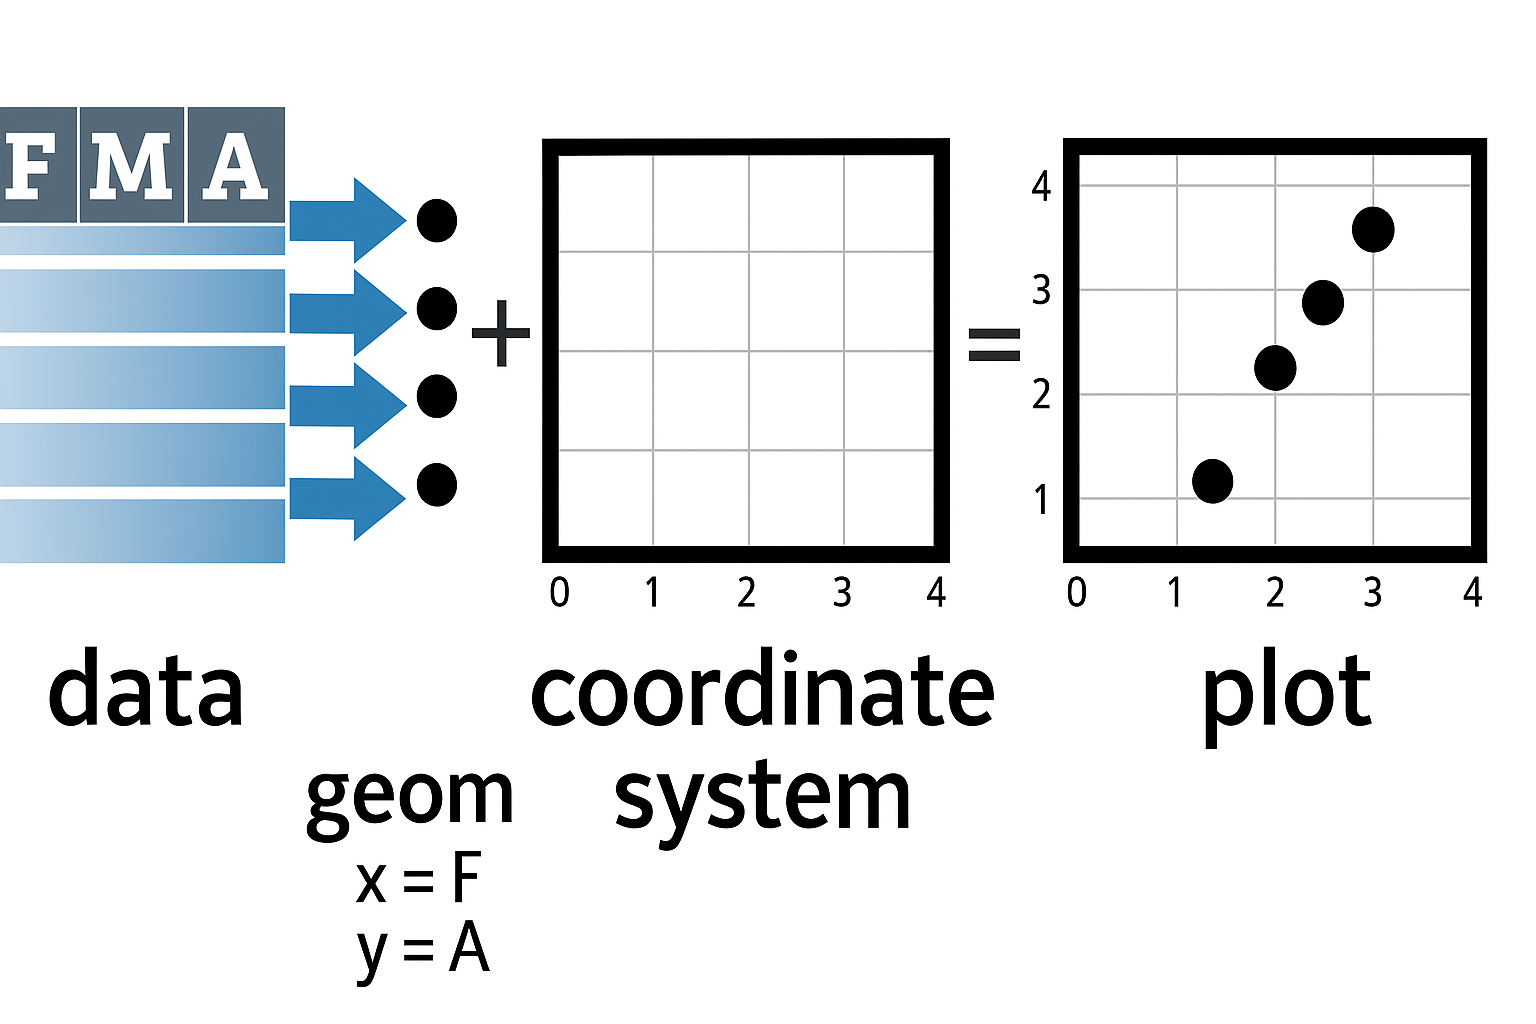
\includegraphics[width=0.5\linewidth,height=\textheight,keepaspectratio]{unidad_1/images/ggplot_estruct.png}
\end{center}

\subsection{\texorpdfstring{Anatomía de gráficos con
\texttt{ggplot2}}{Anatomía de gráficos con ggplot2}}\label{anatomuxeda-de-gruxe1ficos-con-ggplot2}

La estructura básica para construir un gráfico con \texttt{ggplot2} se
organiza a partir de una gramática de gráficos, que se puede entender a
través de sus componentes fundamentales:

\begin{center}
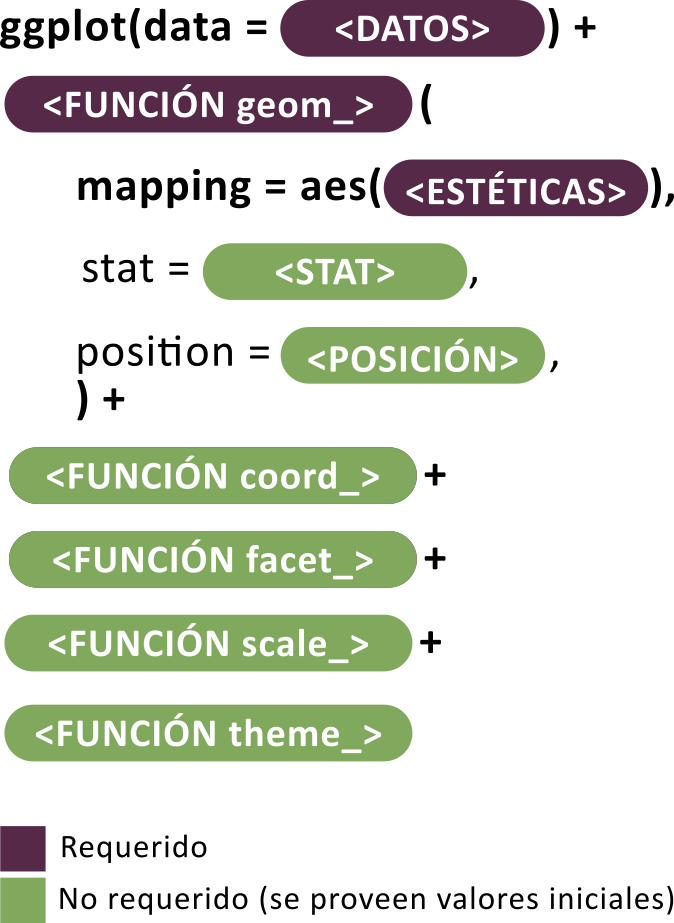
\includegraphics[width=0.55\linewidth,height=\textheight,keepaspectratio]{unidad_1/images/ggplot_comp.png}
\end{center}

\begin{itemize}
\tightlist
\item
  \texttt{data}: el conjunto de datos que vamos a graficar, que debe
  contener toda la información necesaria para crear el gráfico.
\item
  \texttt{aes()}: el mapeo estético (\emph{aesthetic mapping}) es donde
  se declaran las variables que se van a mapear en el gráfico (por
  ejemplo, qué variable va en el eje X, en el eje Y, o cómo se asignan
  los colores).
\item
  \texttt{geoms}: representaciones gráficas de los datos, como puntos,
  líneas, barras, cajas, entre otros. Son los ``objetos geométricos''
  que realmente dibujan el gráfico.
\item
  \texttt{stats}: Transformaciones estadísticas que se realizan sobre
  los datos, como el cálculo de medias, medias móviles o regresiones,
  que ayudan a hacer un resumen de los datos para visualizarlos mejor.
\item
  \texttt{scales}: se utilizan para colorear o escalar los datos según
  distintas variables. Controlan los ejes y las leyendas.
\item
  \texttt{coordinate\ systems}: es el sistema de coordenadas para el
  mapeo del gráfico en un plano bidimensional.
\item
  \texttt{facets}: permiten dividir el conjunto de datos según factores
  y crear gráficos en paneles separados (viñetas), creando matrices
  gráficas.
\item
  \texttt{theme}: son conjuntos de características gráficas que permiten
  controlar la apariencia general de todos los elementos que no son
  datos, como el color del fondo, el tipo de fuente o los bordes.
\end{itemize}

Antes de comenzar a mostrar cómo se usan estos componentes en un
gráfico, leemos la base de datos de ejemplo ``\texttt{facultad.csv}'',
que contiene datos ficticios sobre ingresantes a una facultad (por
ejemplo, sexo, edad, talla y peso). Usaremos este conjunto de datos para
ilustrar los ejemplos gráficos:

\begin{Shaded}
\begin{Highlighting}[]
\CommentTok{\# Cargar datos}
\NormalTok{facultad }\OtherTok{\textless{}{-}} \FunctionTok{read\_csv}\NormalTok{(}\StringTok{"datos/facultad.csv"}\NormalTok{)}

\CommentTok{\# Mostramos las 6 primeras observaciones}
\FunctionTok{head}\NormalTok{(facultad)}
\end{Highlighting}
\end{Shaded}

\begin{verbatim}
# A tibble: 6 x 18
     hc sexo   edad ant_diabetes ant_tbc ant_cancer ant_obesidad ant_ecv ant_ht
  <dbl> <chr> <dbl> <chr>        <chr>   <chr>      <chr>        <chr>   <chr> 
1 26880 M        17 NO           NO      NO         SI           NO      SI    
2 26775 M        18 SI           NO      NO         NO           NO      NO    
3 26877 M        18 SI           NO      SI         NO           NO      SI    
4 26776 M        18 NO           NO      NO         SI           SI      NO    
5 26718 M        18 NO           NO      NO         NO           NO      SI    
6 26738 M        18 NO           NO      NO         NO           NO      SI    
# i 9 more variables: ant_col <chr>, fuma <chr>, edadini <dbl>, cantidad <dbl>,
#   col <dbl>, peso <dbl>, talla <dbl>, sist <dbl>, diast <dbl>
\end{verbatim}

\subsection{\texorpdfstring{Mapeo estético con \texttt{aes()} y capas
geométricas
(\texttt{geom\_})}{Mapeo estético con aes() y capas geométricas (geom\_)}}\label{mapeo-estuxe9tico-con-aes-y-capas-geomuxe9tricas-geom_}

Decíamos que la función \texttt{aes()} hace referencia al contenido
estético del gráfico. Es decir, le brinda indicaciones a
\texttt{ggplot2} sobre cómo dibujar los distintos elementos del gráfico:
líneas, formas, colores y tamaños.

Es importante notar que \texttt{aes()} crea una nueva capa vinculada a
las variables que se desean mapear, y también agrega automáticamente
leyendas cuando corresponde. Al incorporar \texttt{aes()} dentro del
llamado a \texttt{ggplot()}, estamos compartiendo la información
estética con todas las capas del gráfico. Si deseamos que esa
información sólo esté en una de las capas, debemos usar \texttt{aes()}
en la capa correspondiente.

Veamos cómo funciona y cuáles son sus implicancias:

\begin{Shaded}
\begin{Highlighting}[]
\NormalTok{facultad }\SpecialCharTok{|\textgreater{}}
  \CommentTok{\# solo la capa estética aes()}
  \FunctionTok{ggplot}\NormalTok{(}\FunctionTok{aes}\NormalTok{(}\AttributeTok{x =}\NormalTok{ talla, }\AttributeTok{y =}\NormalTok{ peso))}
\end{Highlighting}
\end{Shaded}

\begin{center}
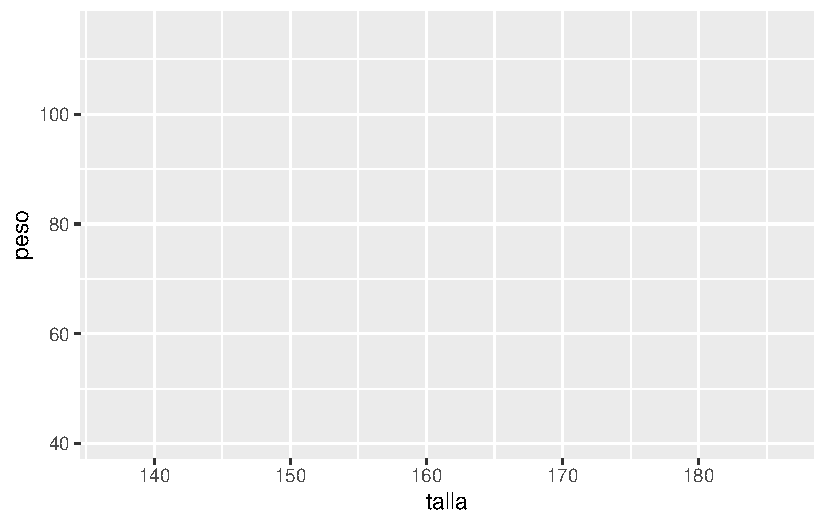
\includegraphics[width=0.85\linewidth,height=\textheight,keepaspectratio]{unidad_1/03_intro_tidyverse_files/figure-pdf/unnamed-chunk-52-1.pdf}
\end{center}

Este código genera un gráfico vacío que contiene únicamente los ejes
especificados (\texttt{peso} y \texttt{talla}), pero aún no muestra los
datos. Para visualizar los puntos, debemos agregar una capa geométrica
usando \texttt{geom\_point()} y enlazarla con el símbolo \texttt{+}:

\begin{Shaded}
\begin{Highlighting}[]
\NormalTok{facultad }\SpecialCharTok{|\textgreater{}}
  \CommentTok{\# mapeo estético}
  \FunctionTok{ggplot}\NormalTok{(}\FunctionTok{aes}\NormalTok{(}\AttributeTok{x =}\NormalTok{ talla, }\AttributeTok{y =}\NormalTok{ peso)) }\SpecialCharTok{+}

  \CommentTok{\# agregamos la capa geométrica de puntos}
  \FunctionTok{geom\_point}\NormalTok{()}
\end{Highlighting}
\end{Shaded}

\begin{center}
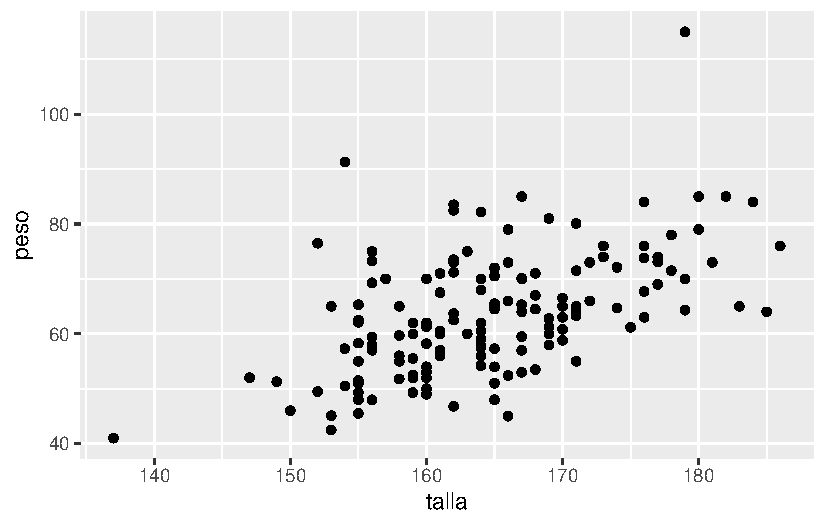
\includegraphics[width=0.85\linewidth,height=\textheight,keepaspectratio]{unidad_1/03_intro_tidyverse_files/figure-pdf/unnamed-chunk-53-1.pdf}
\end{center}

Podemos diferenciar los puntos según sexo incorporando la variable
\texttt{sexo} como argumento del color dentro de \texttt{aes()}:

\begin{Shaded}
\begin{Highlighting}[]
\NormalTok{facultad }\SpecialCharTok{|\textgreater{}}
  \CommentTok{\# mapeo estético}
  \FunctionTok{ggplot}\NormalTok{(}\FunctionTok{aes}\NormalTok{(}\AttributeTok{x =}\NormalTok{ talla, }\AttributeTok{y =}\NormalTok{ peso, }\AttributeTok{color =}\NormalTok{ sexo)) }\SpecialCharTok{+}

  \CommentTok{\# agregamos la capa geométrica de puntos}
  \FunctionTok{geom\_point}\NormalTok{()}
\end{Highlighting}
\end{Shaded}

\begin{center}
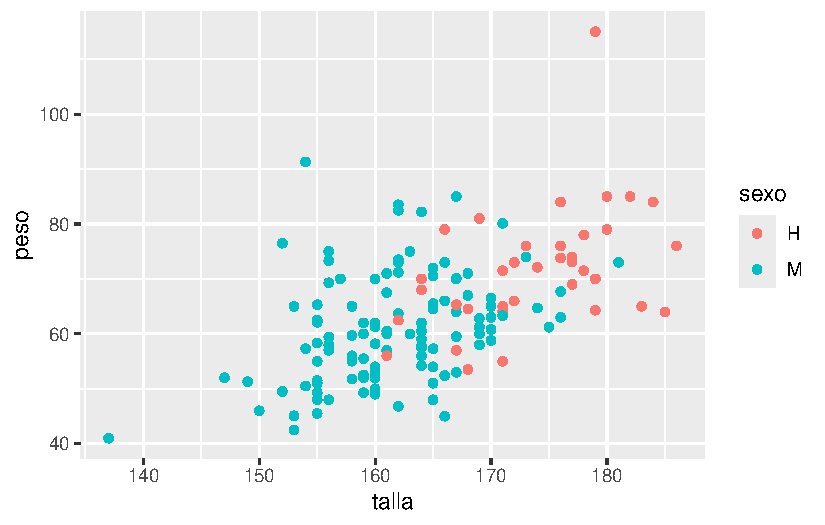
\includegraphics[width=0.85\linewidth,height=\textheight,keepaspectratio]{unidad_1/03_intro_tidyverse_files/figure-pdf/unnamed-chunk-54-1.pdf}
\end{center}

También es posible superponer otras capas geométricas. Por ejemplo,
podemos agregar rectas de regresión para cada grupo según \texttt{sexo}:

\begin{Shaded}
\begin{Highlighting}[]
\NormalTok{facultad }\SpecialCharTok{|\textgreater{}}
  \CommentTok{\# mapeo estético}
  \FunctionTok{ggplot}\NormalTok{(}\FunctionTok{aes}\NormalTok{(}\AttributeTok{x =}\NormalTok{ talla, }\AttributeTok{y =}\NormalTok{ peso, }\AttributeTok{color =}\NormalTok{ sexo)) }\SpecialCharTok{+}

  \CommentTok{\# agregamos la capa geométrica de puntos}
  \FunctionTok{geom\_point}\NormalTok{() }\SpecialCharTok{+}

  \CommentTok{\# agregamos una segunda capa geométrica para la recta de regresión}
  \FunctionTok{geom\_smooth}\NormalTok{(}\AttributeTok{method =} \StringTok{"lm"}\NormalTok{)}
\end{Highlighting}
\end{Shaded}

\begin{center}
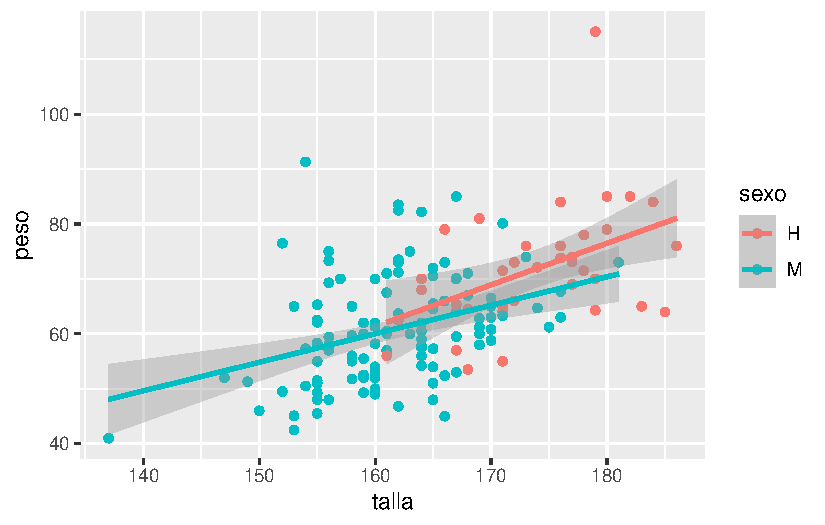
\includegraphics[width=0.85\linewidth,height=\textheight,keepaspectratio]{unidad_1/03_intro_tidyverse_files/figure-pdf/unnamed-chunk-55-1.pdf}
\end{center}

La función \texttt{geom\_smooth()} permite aplicar distintos métodos de
suavizado o ajuste. En este caso usamos \texttt{"lm"} para mostrar la
recta de regresión lineal entre \texttt{talla} y \texttt{peso}, junto
con sus intervalos de confianza.

A continuación, veremos las diferencias entre incluir \texttt{aes()} en
\texttt{ggplot()} (aplicando el mapeo a todo el gráfico) o colocarlo
solo dentro de alguna capa geométrica específica:

\begin{Shaded}
\begin{Highlighting}[]
\NormalTok{facultad }\SpecialCharTok{|\textgreater{}}
  \CommentTok{\# mapeo estético}
  \FunctionTok{ggplot}\NormalTok{(}\FunctionTok{aes}\NormalTok{(}\AttributeTok{x =}\NormalTok{ talla, }\AttributeTok{y =}\NormalTok{ peso)) }\SpecialCharTok{+}

  \CommentTok{\# agregamos la capa geométrica de puntos coloreada por sexo}
  \FunctionTok{geom\_point}\NormalTok{(}\FunctionTok{aes}\NormalTok{(}\AttributeTok{color =}\NormalTok{ sexo)) }\SpecialCharTok{+}

  \CommentTok{\# agregamos una segunda capa geométrica para la recta de regresión}
  \FunctionTok{geom\_smooth}\NormalTok{(}\AttributeTok{method =} \StringTok{"lm"}\NormalTok{)}
\end{Highlighting}
\end{Shaded}

\begin{center}
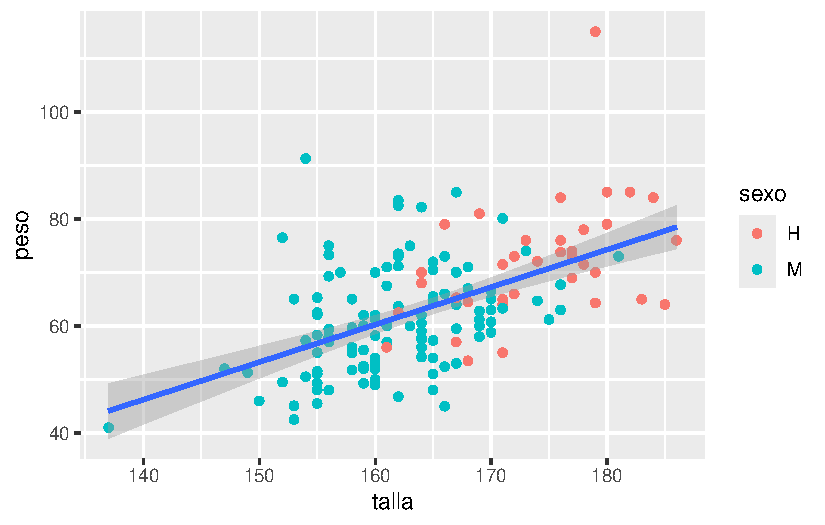
\includegraphics[width=0.85\linewidth,height=\textheight,keepaspectratio]{unidad_1/03_intro_tidyverse_files/figure-pdf/unnamed-chunk-56-1.pdf}
\end{center}

En este ejemplo, el color solo se especifica dentro de
\texttt{geom\_point()}, por lo que los puntos se dibujan diferenciados
por sexo, pero no afecta a la capa de \texttt{geom\_smooth()}
produciendo solo una línea de regresión para el conjunto de puntos.

Este comportamiento brinda gran flexibilidad en la construcción de
gráficos, permitiendo definir qué capas deben responder a qué mapeos
estéticos.

Algunas otras funciones de \texttt{geom\_} son:

\begin{itemize}
\item
  \texttt{geom\_line()}: gráfico de líneas.
\item
  \texttt{geom\_boxplot()}: gráfico de caja y bigotes (\emph{boxplot}).
\item
  \texttt{geom\_histogram()}: histograma.
\item
  \texttt{geom\_density()}: curva de densidad.
\item
  \texttt{geom\_bar()}: gráfico de barras.
\end{itemize}

Todas estas funciones pueden aplicarse sobre los mismos datos, y su uso
depende del objetivo del análisis.

A continuación, algunos ejemplos para visualizar la relación entre
\texttt{sexo} y \texttt{talla} utilizando distintas capas geométricas:

\begin{Shaded}
\begin{Highlighting}[]
\CommentTok{\# Gráfico de puntos}
\NormalTok{facultad }\SpecialCharTok{|\textgreater{}}
  \FunctionTok{ggplot}\NormalTok{(}\FunctionTok{aes}\NormalTok{(}\AttributeTok{x =}\NormalTok{ sexo, }\AttributeTok{y =}\NormalTok{ talla, }\AttributeTok{color =}\NormalTok{ sexo)) }\SpecialCharTok{+}
  \CommentTok{\# capa geométrica de puntos}
  \FunctionTok{geom\_point}\NormalTok{()}
\end{Highlighting}
\end{Shaded}

\begin{center}
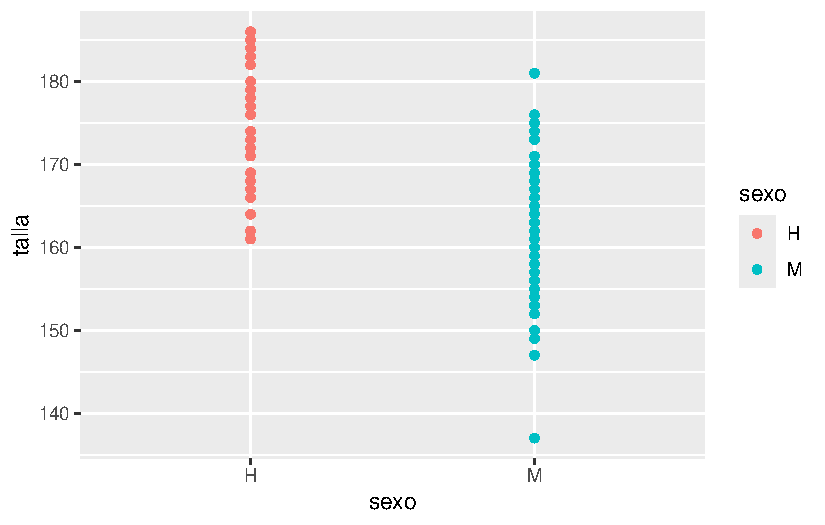
\includegraphics[width=0.85\linewidth,height=\textheight,keepaspectratio]{unidad_1/03_intro_tidyverse_files/figure-pdf/unnamed-chunk-57-1.pdf}
\end{center}

\begin{Shaded}
\begin{Highlighting}[]
\CommentTok{\# Boxplot}
\NormalTok{facultad }\SpecialCharTok{|\textgreater{}}
  \FunctionTok{ggplot}\NormalTok{(}\FunctionTok{aes}\NormalTok{(}\AttributeTok{x =}\NormalTok{ sexo, }\AttributeTok{y =}\NormalTok{ talla, }\AttributeTok{color =}\NormalTok{ sexo)) }\SpecialCharTok{+}
  \CommentTok{\# capa geométrica de boxplot}
  \FunctionTok{geom\_boxplot}\NormalTok{()}
\end{Highlighting}
\end{Shaded}

\begin{center}
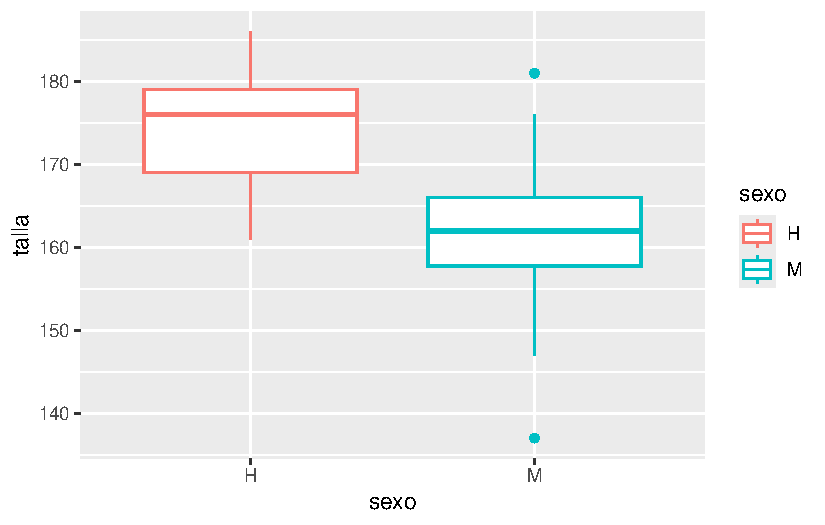
\includegraphics[width=0.85\linewidth,height=\textheight,keepaspectratio]{unidad_1/03_intro_tidyverse_files/figure-pdf/unnamed-chunk-57-2.pdf}
\end{center}

\begin{Shaded}
\begin{Highlighting}[]
\CommentTok{\# Entramado de puntos}
\NormalTok{facultad }\SpecialCharTok{|\textgreater{}}
  \FunctionTok{ggplot}\NormalTok{(}\FunctionTok{aes}\NormalTok{(}\AttributeTok{x =}\NormalTok{ sexo, }\AttributeTok{y =}\NormalTok{ talla, }\AttributeTok{color =}\NormalTok{ sexo)) }\SpecialCharTok{+}
  \CommentTok{\# capa geométrica jitter (entramado de puntos)}
  \FunctionTok{geom\_jitter}\NormalTok{()}
\end{Highlighting}
\end{Shaded}

\begin{center}
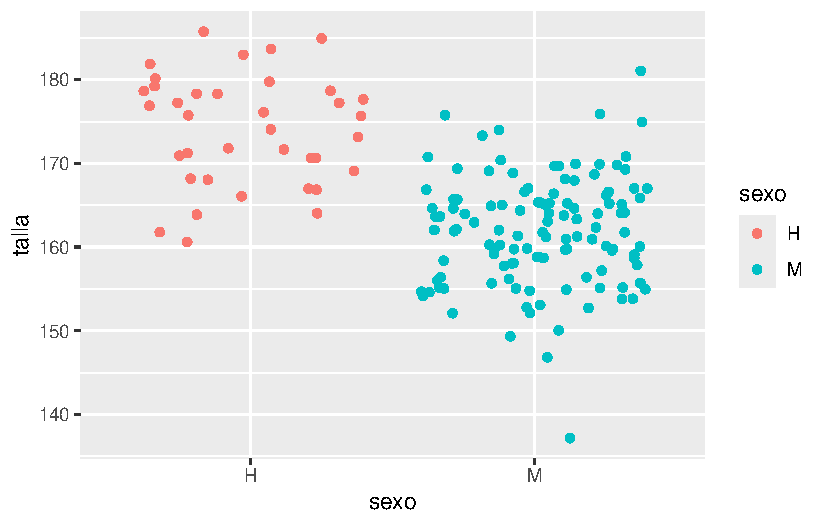
\includegraphics[width=0.85\linewidth,height=\textheight,keepaspectratio]{unidad_1/03_intro_tidyverse_files/figure-pdf/unnamed-chunk-57-3.pdf}
\end{center}

\begin{Shaded}
\begin{Highlighting}[]
\CommentTok{\# Gráfico de violín}
\NormalTok{facultad }\SpecialCharTok{|\textgreater{}}
  \FunctionTok{ggplot}\NormalTok{(}\FunctionTok{aes}\NormalTok{(}\AttributeTok{x =}\NormalTok{ sexo, }\AttributeTok{y =}\NormalTok{ talla, }\AttributeTok{color =}\NormalTok{ sexo)) }\SpecialCharTok{+}
  \CommentTok{\# capa geométrica de violin}
  \FunctionTok{geom\_violin}\NormalTok{()}
\end{Highlighting}
\end{Shaded}

\begin{center}
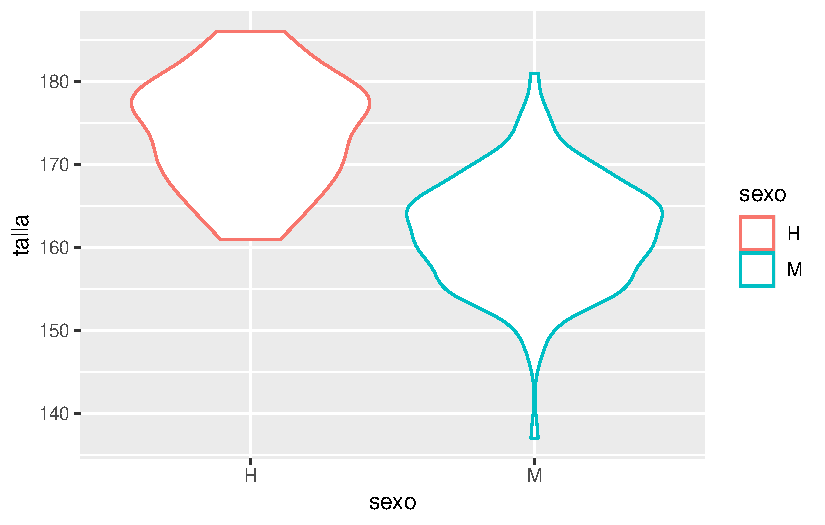
\includegraphics[width=0.85\linewidth,height=\textheight,keepaspectratio]{unidad_1/03_intro_tidyverse_files/figure-pdf/unnamed-chunk-57-4.pdf}
\end{center}

Observemos que en el último gráfico se usó el argumento \texttt{fill} en
lugar de \texttt{color}. Mientras \texttt{color} define el contorno de
líneas, curvas o puntos, \texttt{fill} define el \textbf{relleno} de
objetos geométricos, como los polígonos en gráficos de violín o barras.

\subsection{\texorpdfstring{Personalización de escalas con
\texttt{scale\_}}{Personalización de escalas con scale\_}}\label{personalizaciuxf3n-de-escalas-con-scale_}

El sistema de escalas en \texttt{ggplot2} permite ajustar múltiples
aspectos visuales de un gráfico. Podemos modificar colores de contorno y
relleno, invertir ejes, cambiar tamaños, tipos de línea, entre muchas
otras opciones.

Todas las funciones relacionadas con escalas comienzan con el prefijo
\texttt{scale\_}, seguido del atributo que queremos modificar (por
ejemplo, \texttt{scale\_fill\_} para cambiar el color de relleno).

A continuación, mostramos algunos ejemplos aplicados sobre el conjunto
de datos \texttt{facultad}:

\begin{Shaded}
\begin{Highlighting}[]
\NormalTok{facultad }\SpecialCharTok{|\textgreater{}}
  \FunctionTok{ggplot}\NormalTok{(}\FunctionTok{aes}\NormalTok{(}\AttributeTok{x =}\NormalTok{ sexo, }\AttributeTok{y =}\NormalTok{ talla, }\AttributeTok{fill =}\NormalTok{ sexo)) }\SpecialCharTok{+}

  \CommentTok{\# capa geométrica boxplot}
  \FunctionTok{geom\_boxplot}\NormalTok{() }\SpecialCharTok{+}

  \CommentTok{\# paleta de naranjas}
  \FunctionTok{scale\_fill\_brewer}\NormalTok{(}\AttributeTok{palette =} \StringTok{"Oranges"}\NormalTok{)}
\end{Highlighting}
\end{Shaded}

\begin{center}
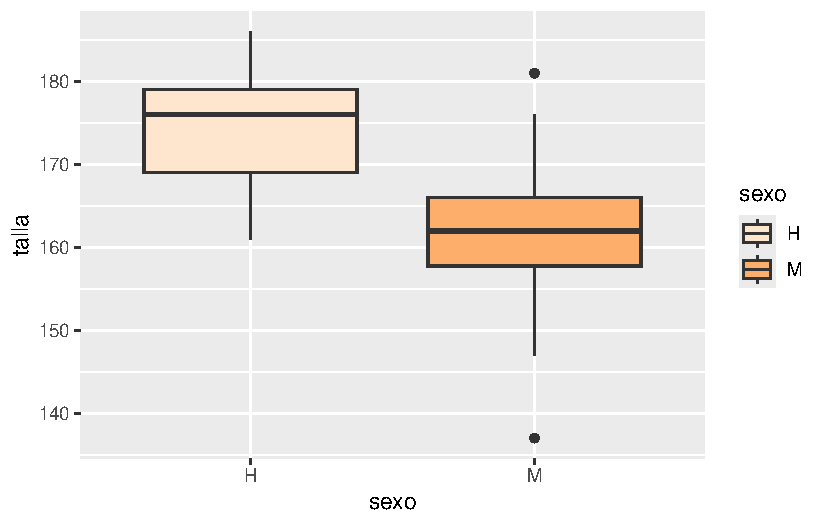
\includegraphics[width=0.85\linewidth,height=\textheight,keepaspectratio]{unidad_1/03_intro_tidyverse_files/figure-pdf/unnamed-chunk-58-1.pdf}
\end{center}

En este ejemplo aplicamos una capa \texttt{scale\_fill\_brewer()} con la
paleta de colores \texttt{"Oranges"} que se vincula con el argumento
\texttt{fill} de \texttt{aes()} y definen los colores del
\emph{boxplot}.

Otra alternativa es aplicar una escala de grises mediante
\texttt{scale\_fill\_grey()}:

\begin{Shaded}
\begin{Highlighting}[]
\NormalTok{facultad }\SpecialCharTok{|\textgreater{}}
  \FunctionTok{ggplot}\NormalTok{(}\FunctionTok{aes}\NormalTok{(}\AttributeTok{x =}\NormalTok{ sexo, }\AttributeTok{y =}\NormalTok{ talla, }\AttributeTok{fill =}\NormalTok{ sexo)) }\SpecialCharTok{+}

  \CommentTok{\# capa geométrica boxplot}
  \FunctionTok{geom\_boxplot}\NormalTok{() }\SpecialCharTok{+}

  \CommentTok{\# paleta en escala de grises}
  \FunctionTok{scale\_fill\_grey}\NormalTok{(}\AttributeTok{start =} \FloatTok{0.4}\NormalTok{, }\AttributeTok{end =} \FloatTok{0.8}\NormalTok{)}
\end{Highlighting}
\end{Shaded}

\begin{center}
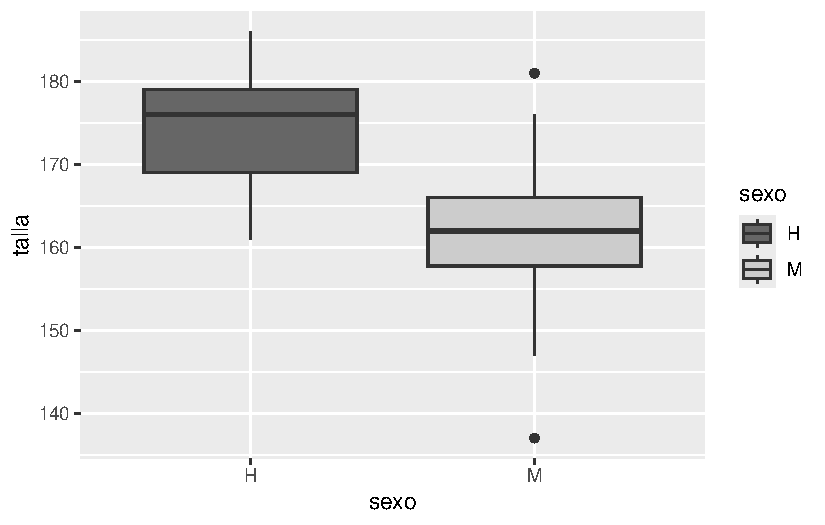
\includegraphics[width=0.85\linewidth,height=\textheight,keepaspectratio]{unidad_1/03_intro_tidyverse_files/figure-pdf/unnamed-chunk-59-1.pdf}
\end{center}

\begin{quote}
Recomendamos trabajar con paletas de colores accesibles para personas
con daltonismo y otras discapacidades visuales, como las incluidas en
las dependencias \texttt{RColorBrewer}{[}@RColorBrewer{]} y
\texttt{viridisLite}, así como en paquetes específicos con paletas
\emph{colorblind-friendly}, como \texttt{scico} {[}@scico{]}.
\end{quote}

También podemos modificar las escalas de los ejes. Por ejemplo, invertir
el eje X con \texttt{scale\_x\_reverse()}:

\begin{Shaded}
\begin{Highlighting}[]
\NormalTok{facultad }\SpecialCharTok{|\textgreater{}}
  \FunctionTok{ggplot}\NormalTok{(}\FunctionTok{aes}\NormalTok{(}\AttributeTok{x =}\NormalTok{ talla, }\AttributeTok{y =}\NormalTok{ peso, }\AttributeTok{fill =}\NormalTok{ sexo)) }\SpecialCharTok{+}

  \CommentTok{\# capa geométrica de puntos}
  \FunctionTok{geom\_point}\NormalTok{() }\SpecialCharTok{+}

  \CommentTok{\# invierte el eje x}
  \FunctionTok{scale\_x\_reverse}\NormalTok{()}
\end{Highlighting}
\end{Shaded}

\begin{center}
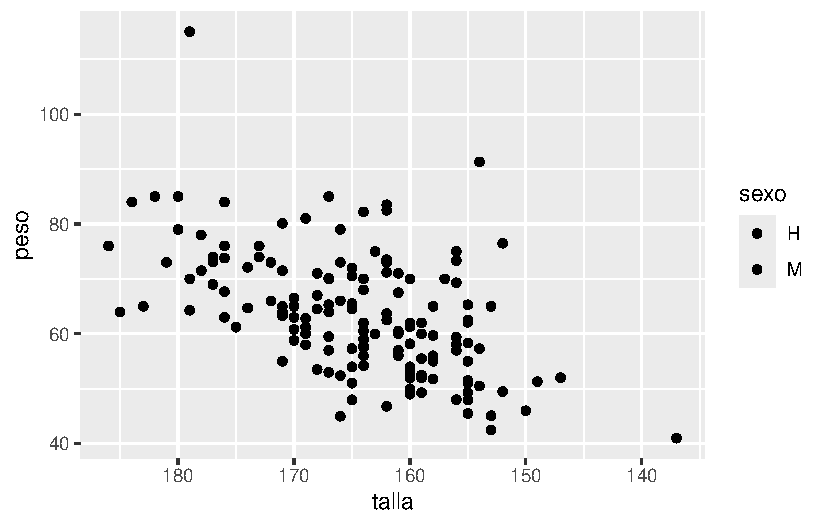
\includegraphics[width=0.85\linewidth,height=\textheight,keepaspectratio]{unidad_1/03_intro_tidyverse_files/figure-pdf/unnamed-chunk-60-1.pdf}
\end{center}

La inclusión de \texttt{scale\_x\_reverse()} provoca la variable
\texttt{talla} se muestre en orden descendente, de mayor a menor.

Por último, podemos personalizar los cortes del eje Y utilizando
\texttt{scale\_y\_continuous()}. Por ejemplo, en el \emph{boxplot}
pintado en escala de grises, definimos que el eje Y comienza en 130cm y
termina en 200cm, con cortes cada 5cm y etiquetas cada 10cm:

\begin{Shaded}
\begin{Highlighting}[]
\NormalTok{facultad }\SpecialCharTok{|\textgreater{}}
  \FunctionTok{ggplot}\NormalTok{(}\FunctionTok{aes}\NormalTok{(}\AttributeTok{x =}\NormalTok{ sexo, }\AttributeTok{y =}\NormalTok{ talla, }\AttributeTok{fill =}\NormalTok{ sexo)) }\SpecialCharTok{+}

  \CommentTok{\# capa geométrica boxplot}
  \FunctionTok{geom\_boxplot}\NormalTok{() }\SpecialCharTok{+}

  \CommentTok{\# paleta en escala de grises}
  \FunctionTok{scale\_fill\_grey}\NormalTok{(}\AttributeTok{start =} \FloatTok{0.4}\NormalTok{, }\AttributeTok{end =} \FloatTok{0.8}\NormalTok{) }\SpecialCharTok{+}

  \CommentTok{\# puntos de corte del eje Y}
  \FunctionTok{scale\_y\_continuous}\NormalTok{(}
    \AttributeTok{limits =} \FunctionTok{c}\NormalTok{(}\DecValTok{130}\NormalTok{, }\DecValTok{200}\NormalTok{), }\CommentTok{\# límites}
    \AttributeTok{breaks =} \FunctionTok{seq}\NormalTok{(}\DecValTok{130}\NormalTok{, }\DecValTok{200}\NormalTok{, }\DecValTok{10}\NormalTok{)}
\NormalTok{  ) }\CommentTok{\# nro de etiquetas}
\end{Highlighting}
\end{Shaded}

\begin{center}
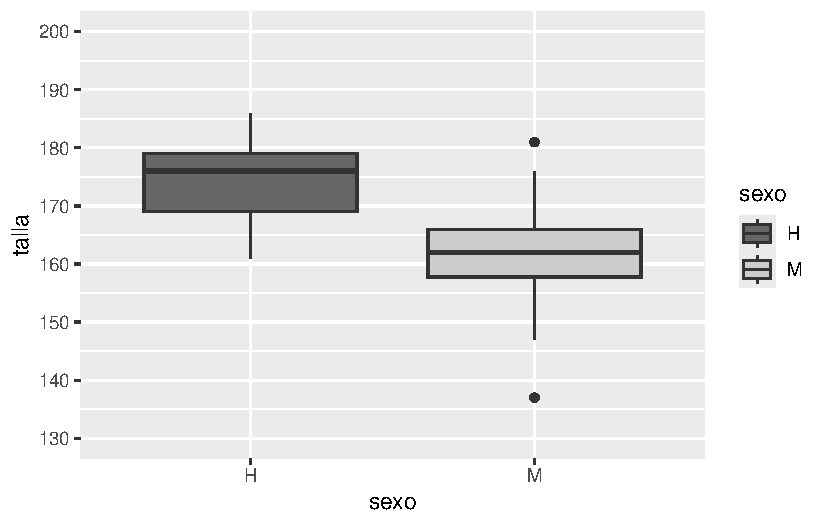
\includegraphics[width=0.85\linewidth,height=\textheight,keepaspectratio]{unidad_1/03_intro_tidyverse_files/figure-pdf/unnamed-chunk-61-1.pdf}
\end{center}

\subsection{\texorpdfstring{Transformaciones estadísticas con
\textbf{\texttt{stat\_}}}{Transformaciones estadísticas con stat\_}}\label{transformaciones-estaduxedsticas-con-stat_}

Algunos gráficos en \texttt{ggplot2} no requieren transformaciones
estadísticas, como los gráficos de dispersión. Sin embargo, otros tipos
---como \emph{boxplots}, histogramas o líneas de tendencia--- sí aplican
transformaciones estadísticas predeterminadas que pueden ser modificadas
o personalizadas.

Estas transformaciones pueden formar parte de las funciones geométricas,
como ocurre en los histogramas, o agregarse como capas independientes
mediante funciones \texttt{stat\_}.

Por ejemplo, en los histogramas podemos definir la cantidad de
intervalos (o ``clases'') a través del argumento \texttt{bins}, que
forma parte de \texttt{geom\_histogram()}:

\begin{Shaded}
\begin{Highlighting}[]
\NormalTok{facultad }\SpecialCharTok{|\textgreater{}}
  \FunctionTok{ggplot}\NormalTok{(}\FunctionTok{aes}\NormalTok{(edad)) }\SpecialCharTok{+}

  \CommentTok{\# capa geométrica histograma}
  \FunctionTok{geom\_histogram}\NormalTok{(}\AttributeTok{bins =} \FunctionTok{nclass.Sturges}\NormalTok{(facultad}\SpecialCharTok{$}\NormalTok{edad), }\AttributeTok{fill =} \StringTok{"Blue"}\NormalTok{)}
\end{Highlighting}
\end{Shaded}

\begin{center}
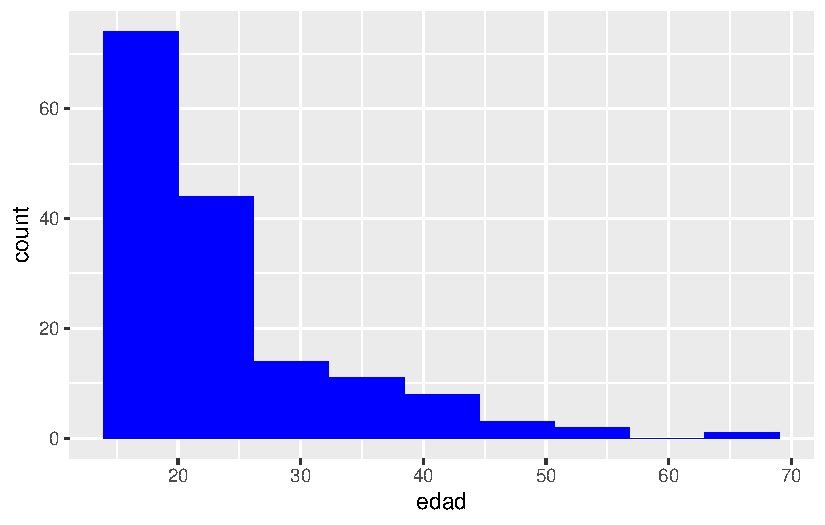
\includegraphics[width=0.85\linewidth,height=\textheight,keepaspectratio]{unidad_1/03_intro_tidyverse_files/figure-pdf/unnamed-chunk-62-1.pdf}
\end{center}

En este caso, utilizamos la regla de Sturges ---a través de la función
\texttt{nclass.Sturges()}--- para determinar automáticamente la cantidad
de clases para la variable \texttt{edad}.

También podemos superponer al gráfico transformaciones estadísticas como
capas adicionales. Por ejemplo, si deseamos agregar la media de
\texttt{talla} en cada grupo de \texttt{sexo} sobre un \emph{boxplot},
utilizamos \texttt{stat\_summary()}:

\begin{Shaded}
\begin{Highlighting}[]
\NormalTok{facultad }\SpecialCharTok{|\textgreater{}}
  \FunctionTok{ggplot}\NormalTok{(}\FunctionTok{aes}\NormalTok{(}\AttributeTok{x =}\NormalTok{ sexo, }\AttributeTok{y =}\NormalTok{ talla, }\AttributeTok{fill =}\NormalTok{ sexo)) }\SpecialCharTok{+}

  \CommentTok{\# capa geométrica boxplot}
  \FunctionTok{geom\_boxplot}\NormalTok{() }\SpecialCharTok{+}

  \CommentTok{\# paleta de tonos verdes}
  \FunctionTok{scale\_fill\_brewer}\NormalTok{(}\AttributeTok{palette =} \StringTok{"Greens"}\NormalTok{) }\SpecialCharTok{+}

  \CommentTok{\# añade capa summary}
  \FunctionTok{stat\_summary}\NormalTok{(}
    \AttributeTok{fun =}\NormalTok{ mean,}
    \AttributeTok{color =} \StringTok{"darkred"}\NormalTok{,}
    \AttributeTok{geom =} \StringTok{"point"}\NormalTok{,}
    \AttributeTok{shape =} \DecValTok{18}\NormalTok{,}
    \AttributeTok{size =} \DecValTok{3}
\NormalTok{  )}
\end{Highlighting}
\end{Shaded}

\begin{center}
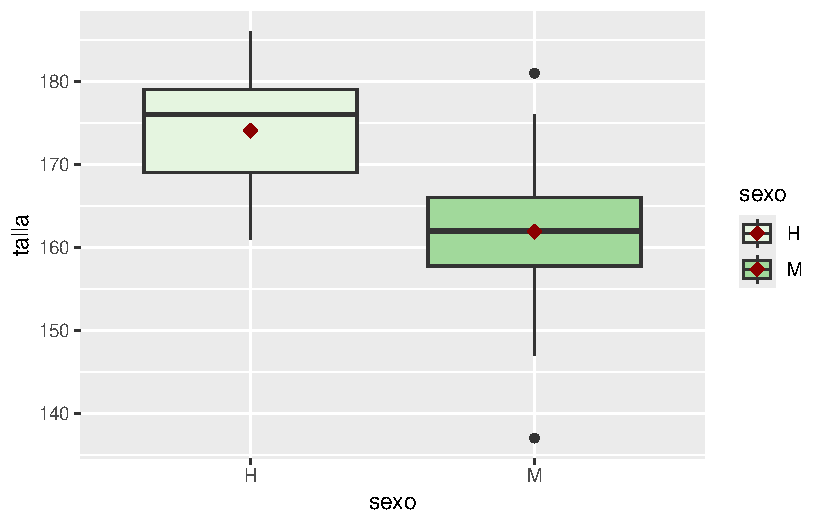
\includegraphics[width=0.85\linewidth,height=\textheight,keepaspectratio]{unidad_1/03_intro_tidyverse_files/figure-pdf/unnamed-chunk-63-1.pdf}
\end{center}

La función \texttt{stat\_summary()} permite aplicar funciones
estadísticas como \texttt{mean}, \texttt{median}, \texttt{sd}, entre
otras, y representar el resultado con un objeto geométrico, en este caso
\texttt{geom\ =\ "point"}. En el gráfico, la media de \texttt{talla} se
muestra con un punto rojo oscuro (\texttt{color\ =\ "darkred"}), de
forma romboidal (\texttt{shape\ =\ 18}) y tamaño ampliado
(\texttt{size\ =\ 3}).

\subsection{\texorpdfstring{Facetado con
\textbf{\texttt{facet\_}}}{Facetado con facet\_}}\label{facetado-con-facet_}

El facetado permite dividir un gráfico en múltiples paneles o viñetas
según los niveles de una o más variables categóricas. Esto resulta
especialmente útil cuando se desea comparar patrones entre grupos sin
sobrecargar un único gráfico con demasiada información.

\texttt{ggplot2} ofrece dos funciones principales para realizar esta
tarea:

\begin{itemize}
\item
  \texttt{facet\_wrap()}: separa los datos según \textbf{una única
  variable categórica}, generando una serie de paneles dispuestos de
  forma automática en filas y columnas.
\item
  \texttt{facet\_grid()}: permite crear una \textbf{matriz de paneles}
  cruzando \textbf{dos variables categóricas}, una para las filas y otra
  para las columnas.
\end{itemize}

Retomemos el gráfico de dispersión entre \texttt{talla} y \texttt{peso},
y generemos paneles separados para cada nivel de la variable
\texttt{sexo} con \texttt{facet\_wrap()}:

\begin{Shaded}
\begin{Highlighting}[]
\NormalTok{facultad }\SpecialCharTok{|\textgreater{}}

  \FunctionTok{ggplot}\NormalTok{(}\FunctionTok{aes}\NormalTok{(}\AttributeTok{x =}\NormalTok{ talla, }\AttributeTok{y =}\NormalTok{ peso, }\AttributeTok{color =}\NormalTok{ sexo)) }\SpecialCharTok{+}

  \CommentTok{\# capa geométrica de puntos}
  \FunctionTok{geom\_point}\NormalTok{() }\SpecialCharTok{+}

  \CommentTok{\# separa en paneles por sexo}
  \FunctionTok{facet\_wrap}\NormalTok{(}\SpecialCharTok{\textasciitilde{}}\NormalTok{sexo)}
\end{Highlighting}
\end{Shaded}

\begin{center}
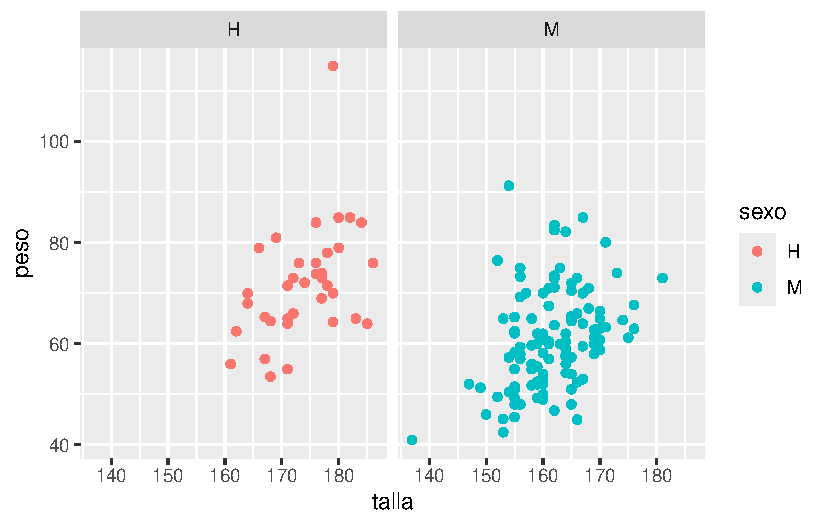
\includegraphics[width=0.85\linewidth,height=\textheight,keepaspectratio]{unidad_1/03_intro_tidyverse_files/figure-pdf/unnamed-chunk-64-1.pdf}
\end{center}

Usaremos \texttt{facet\_grid()} para crear una matriz de histogramas
producto del cruce de las variables \texttt{fuma} y \texttt{sexo}.
Dentro de la cuadrícula graficaremos histogramas de la variable
\texttt{peso} coloreados por \texttt{sexo}:

\begin{Shaded}
\begin{Highlighting}[]
\NormalTok{facultad }\SpecialCharTok{|\textgreater{}}
  \FunctionTok{ggplot}\NormalTok{(}\FunctionTok{aes}\NormalTok{(}\AttributeTok{y =}\NormalTok{ peso, }\AttributeTok{fill =}\NormalTok{ sexo)) }\SpecialCharTok{+}

  \CommentTok{\# capa geométrica histograma}
  \FunctionTok{geom\_histogram}\NormalTok{(}\AttributeTok{bins =} \FunctionTok{nclass.Sturges}\NormalTok{(facultad}\SpecialCharTok{$}\NormalTok{peso)) }\SpecialCharTok{+}

  \CommentTok{\# paleta de colores}
  \FunctionTok{scale\_fill\_brewer}\NormalTok{(}\AttributeTok{palette =} \StringTok{"Set1"}\NormalTok{) }\SpecialCharTok{+}

  \CommentTok{\# separa en paneles por sexo y fuma}
  \FunctionTok{facet\_grid}\NormalTok{(sexo }\SpecialCharTok{\textasciitilde{}}\NormalTok{ fuma)}
\end{Highlighting}
\end{Shaded}

\begin{center}
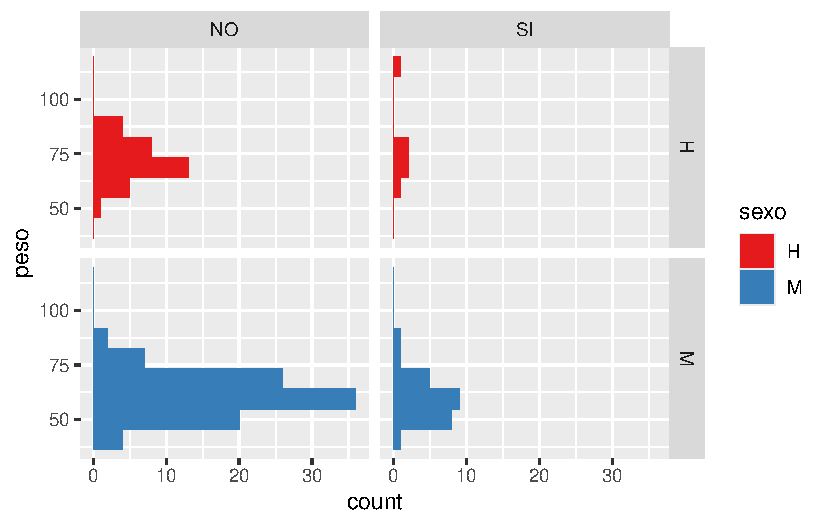
\includegraphics[width=0.85\linewidth,height=\textheight,keepaspectratio]{unidad_1/03_intro_tidyverse_files/figure-pdf/unnamed-chunk-65-1.pdf}
\end{center}

Como se puede ver en estos ejemplos, estamos integrando varias de las
funciones vistas: mapeo estético, capas geométricas, escalas, y ahora
también el facetado.

El número de combinaciones posibles es enorme, dada la variedad de
funciones y argumentos que ofrece \texttt{ggplot2}. Sin embargo, el
objetivo de este material es comprender los principios fundamentales
sobre los que se construye esta ``\emph{gramática de los gráficos}'',
propuesta por los autores del paquete.

\subsection{\texorpdfstring{Sistema de coordenadas con
\texttt{coord\_}}{Sistema de coordenadas con coord\_}}\label{sistema-de-coordenadas-con-coord_}

En algunas ocasiones, puede ser útil modificar el sistema de coordenadas
predeterminado del gráfico. Por ejemplo, para invertir los ejes y
presentar un gráfico de barras en disposición horizontal:

\begin{Shaded}
\begin{Highlighting}[]
\NormalTok{facultad }\SpecialCharTok{|\textgreater{}}

  \FunctionTok{ggplot}\NormalTok{(}\FunctionTok{aes}\NormalTok{(sexo, }\AttributeTok{fill =}\NormalTok{ sexo)) }\SpecialCharTok{+}

  \CommentTok{\# capa geométrica barras}
  \FunctionTok{geom\_bar}\NormalTok{() }\SpecialCharTok{+}

  \CommentTok{\# paleta de colores}
  \FunctionTok{scale\_fill\_brewer}\NormalTok{(}\AttributeTok{palette =} \StringTok{"Set2"}\NormalTok{) }\SpecialCharTok{+}

  \CommentTok{\# invierte disposición de ejes}
  \FunctionTok{coord\_flip}\NormalTok{()}
\end{Highlighting}
\end{Shaded}

\begin{center}
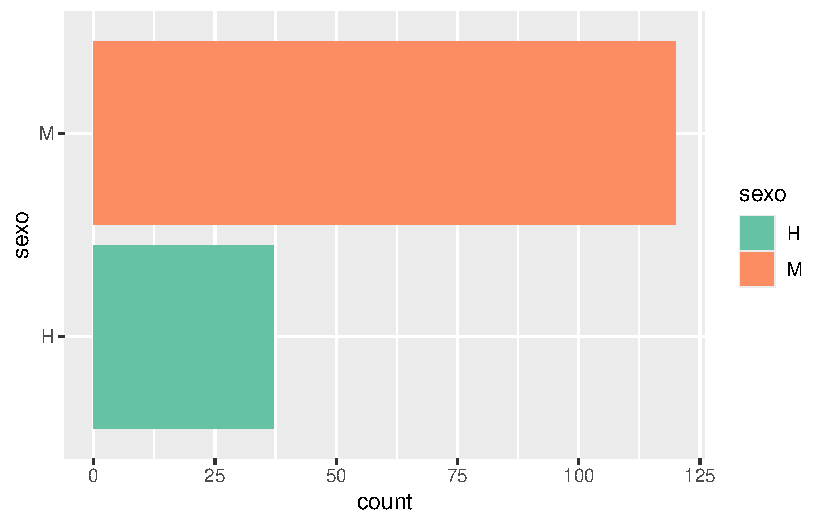
\includegraphics[width=0.85\linewidth,height=\textheight,keepaspectratio]{unidad_1/03_intro_tidyverse_files/figure-pdf/unnamed-chunk-66-1.pdf}
\end{center}

\subsection{\texorpdfstring{Temas con
\texttt{theme()}}{Temas con theme()}}\label{temas-con-theme}

\texttt{ggplot2} incluye un conjunto de temas gráficos predefinidos que
permiten modificar el aspecto general del gráfico. El tema por defecto
es \texttt{theme\_gray()}, pero puede cambiarse agregando una capa
\texttt{theme\_*()} dentro del gráfico.

Repetimos el gráfico anterior, esta vez utilizando el tema blanco y
negro (\texttt{theme\_bw()}):

\begin{Shaded}
\begin{Highlighting}[]
\NormalTok{facultad }\SpecialCharTok{|\textgreater{}}

  \FunctionTok{ggplot}\NormalTok{(}\FunctionTok{aes}\NormalTok{(sexo, }\AttributeTok{fill =}\NormalTok{ sexo)) }\SpecialCharTok{+}

  \CommentTok{\# capa geométrica barras}
  \FunctionTok{geom\_bar}\NormalTok{() }\SpecialCharTok{+}

  \CommentTok{\# paleta de colores}
  \FunctionTok{scale\_fill\_brewer}\NormalTok{(}\AttributeTok{palette =} \StringTok{"Set2"}\NormalTok{) }\SpecialCharTok{+}

  \CommentTok{\# invierte disposición de ejes}
  \FunctionTok{coord\_flip}\NormalTok{() }\SpecialCharTok{+}

  \CommentTok{\# tema en blanco y negro}
  \FunctionTok{theme\_bw}\NormalTok{()}
\end{Highlighting}
\end{Shaded}

\begin{center}
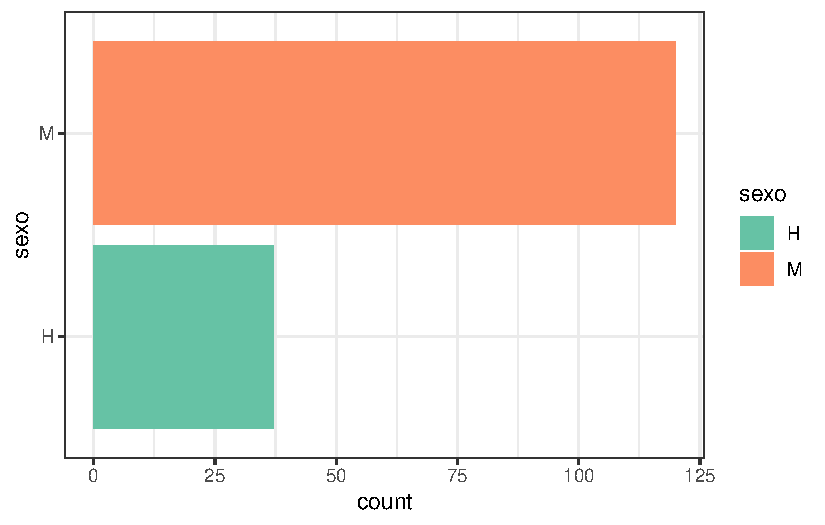
\includegraphics[width=0.85\linewidth,height=\textheight,keepaspectratio]{unidad_1/03_intro_tidyverse_files/figure-pdf/unnamed-chunk-67-1.pdf}
\end{center}

También podemos aplicar un tema de fondo oscuro con
\texttt{theme\_dark()}:

\begin{Shaded}
\begin{Highlighting}[]
\NormalTok{facultad }\SpecialCharTok{|\textgreater{}}

  \FunctionTok{ggplot}\NormalTok{(}\FunctionTok{aes}\NormalTok{(sexo, }\AttributeTok{fill =}\NormalTok{ sexo)) }\SpecialCharTok{+}

  \CommentTok{\# capa geométrica barras}
  \FunctionTok{geom\_bar}\NormalTok{() }\SpecialCharTok{+}

  \CommentTok{\# paleta de colores}
  \FunctionTok{scale\_fill\_brewer}\NormalTok{(}\AttributeTok{palette =} \StringTok{"Set2"}\NormalTok{) }\SpecialCharTok{+}

  \CommentTok{\# invierte disposición de ejes}
  \FunctionTok{coord\_flip}\NormalTok{() }\SpecialCharTok{+}

  \CommentTok{\# tema con fondo oscuro}
  \FunctionTok{theme\_dark}\NormalTok{()}
\end{Highlighting}
\end{Shaded}

\begin{center}
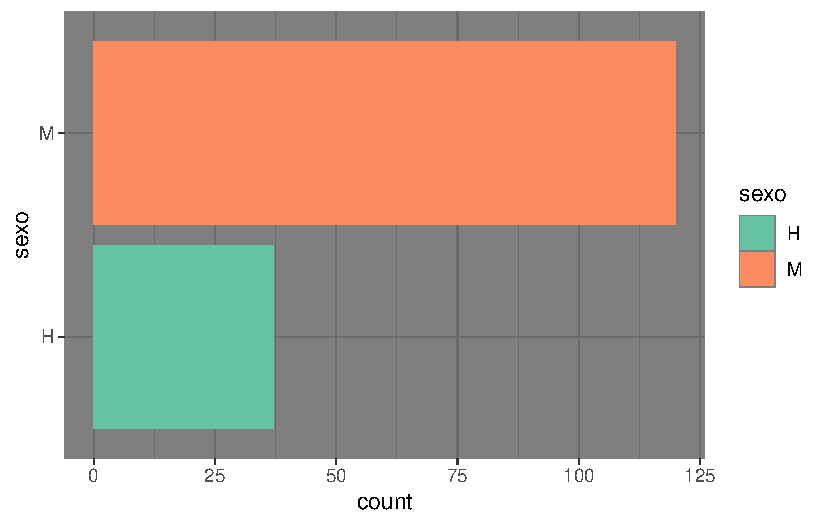
\includegraphics[width=0.85\linewidth,height=\textheight,keepaspectratio]{unidad_1/03_intro_tidyverse_files/figure-pdf/unnamed-chunk-68-1.pdf}
\end{center}

A continuación se muestra un cuadro con los principales temas
disponibles en \texttt{ggplot2} y sus características visuales:

\begin{center}
\pandocbounded{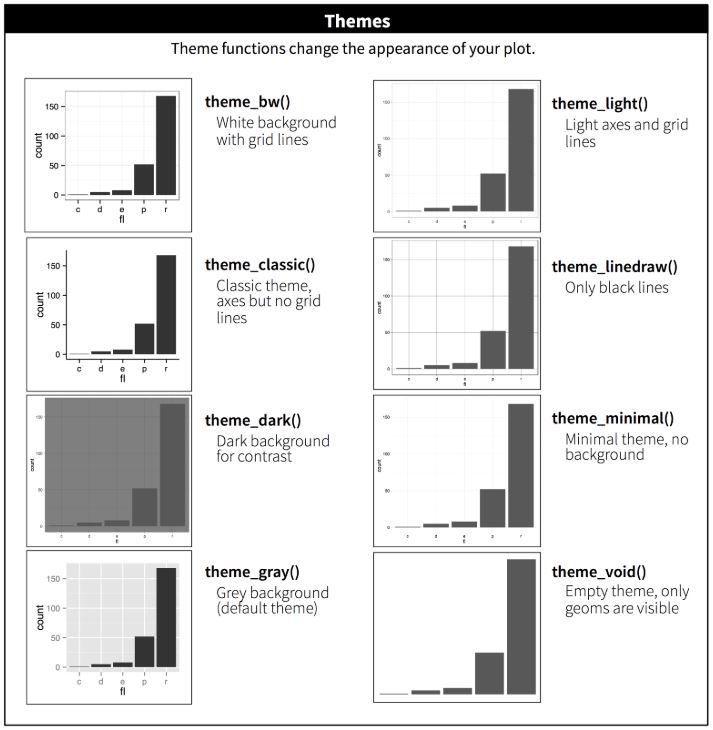
\includegraphics[keepaspectratio]{unidad_1/images/ggplot_temas.JPG}}
\end{center}

Además del aspecto general del gráfico, es posible agregar títulos,
subtítulos y etiquetas de ejes con la función \texttt{labs()}. Por
ejemplo:

\begin{Shaded}
\begin{Highlighting}[]
\FunctionTok{labs}\NormalTok{(}
  \AttributeTok{x =} \StringTok{"Etiqueta X"}\NormalTok{,}
  \AttributeTok{y =} \StringTok{"Etiqueta Y"}\NormalTok{,}
  \AttributeTok{title =} \StringTok{"Título del gráfico"}\NormalTok{,}
  \AttributeTok{subtitle =} \StringTok{"Subtítulo del gráfico"}
\NormalTok{)}
\end{Highlighting}
\end{Shaded}

También se pueden ajustar detalles del texto, como tipo de fuente o
tamaño, mediante la función \texttt{theme()}:

\begin{Shaded}
\begin{Highlighting}[]
\NormalTok{facultad }\SpecialCharTok{|\textgreater{}}
  \FunctionTok{ggplot}\NormalTok{(}\FunctionTok{aes}\NormalTok{(sexo, }\AttributeTok{fill =}\NormalTok{ sexo)) }\SpecialCharTok{+}
  \CommentTok{\# capa geométrica barras}
  \FunctionTok{geom\_bar}\NormalTok{() }\SpecialCharTok{+}
  \CommentTok{\# paleta de colores}
  \FunctionTok{scale\_fill\_brewer}\NormalTok{(}\AttributeTok{palette =} \StringTok{"Set2"}\NormalTok{) }\SpecialCharTok{+}
  \CommentTok{\# invierte disposición de ejes}
  \FunctionTok{coord\_flip}\NormalTok{() }\SpecialCharTok{+}
  \CommentTok{\# cambia etiquetas de los ejes}
  \FunctionTok{labs}\NormalTok{(}\AttributeTok{y =} \StringTok{"Cantidad"}\NormalTok{, }\AttributeTok{title =} \StringTok{"Distribución de sexo"}\NormalTok{) }\SpecialCharTok{+}
  \CommentTok{\# modifica el estilo de fuente del título}
  \FunctionTok{theme}\NormalTok{(}\AttributeTok{plot.title =} \FunctionTok{element\_text}\NormalTok{(}\AttributeTok{face =} \StringTok{"italic"}\NormalTok{, }\AttributeTok{size =} \DecValTok{16}\NormalTok{))}
\end{Highlighting}
\end{Shaded}

\begin{center}
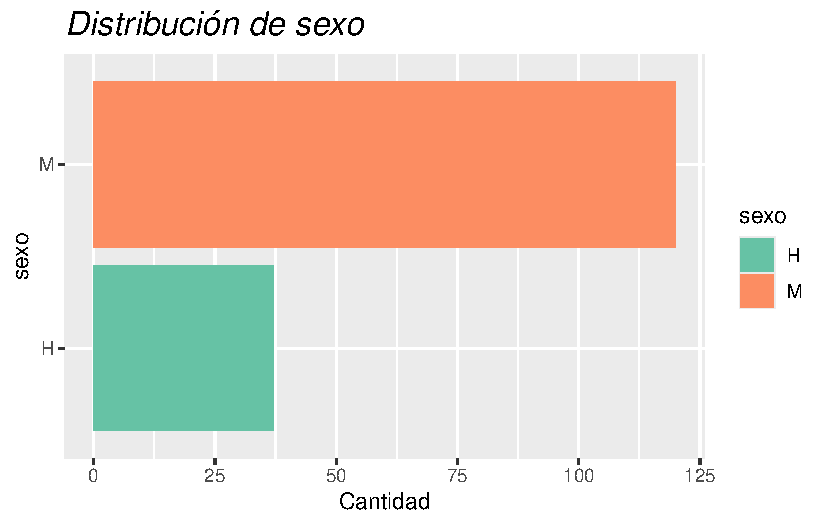
\includegraphics[width=0.85\linewidth,height=\textheight,keepaspectratio]{unidad_1/03_intro_tidyverse_files/figure-pdf/unnamed-chunk-70-1.pdf}
\end{center}

\subsection{\texorpdfstring{Paquete
\texttt{esquisse}}{Paquete esquisse}}\label{paquete-esquisse}

\begin{center}

\includegraphics[width=0.2\linewidth,height=\textheight,keepaspectratio]{unidad_1/images/esquisse.PNG}
\end{center}

El paquete\texttt{esquisse} {[}@esquisse{]} es una extensión de
\texttt{ggplot2} que permite crear gráficos de manera interactiva,
mediante una interfaz gráfica intuitiva basada en el sistema de
arrastrar y soltar (\emph{drag \& drop}).

Con \texttt{esquisse} es posible:

\begin{itemize}
\item
  Explorar visualmente los datos según su tipo.
\item
  Asignar variables a diferentes estéticas del gráfico (ejes, color,
  tamaño, etc.).
\item
  Exportar los resultados en distintos formatos.
\item
  Recuperar el código R que genera el gráfico, facilitando su
  reproducción y modificación.
\end{itemize}

El paquete se instala mediante el menú \textbf{Packages} de RStudio o
ejecutando:

\begin{Shaded}
\begin{Highlighting}[]
\FunctionTok{install.packages}\NormalTok{(}\StringTok{"esquisse"}\NormalTok{)}
\end{Highlighting}
\end{Shaded}

Luego se puede acceder a la aplicación por medio del acceso Addins:

\begin{center}
\pandocbounded{
\includegraphics[keepaspectratio]{unidad_1/images/addins.png}}
\end{center}

o ejecutando en consola:

\begin{Shaded}
\begin{Highlighting}[]
\FunctionTok{esquisser}\NormalTok{()}
\end{Highlighting}
\end{Shaded}

También se puede agregar el nombre de la tabla de datos dentro de los
paréntesis

\begin{Shaded}
\begin{Highlighting}[]
\FunctionTok{esquisser}\NormalTok{(datos)}
\end{Highlighting}
\end{Shaded}

Para más detalles, se puede consultar la
\href{https://cran.r-project.org/web/packages/esquisse/vignettes/get-started.html}{viñeta}
del paquete disponible en CRAN o en su
\href{https://github.com/dreamRs/esquisse}{repositorio de GitHub}.

\subsection{Otras extensiones de
ggplot2}\label{otras-extensiones-de-ggplot2}

Una de las grandes fortalezas de \texttt{ggplot2} es su ecosistema de
extensiones. Hasta el momento, existen más de
\href{https://exts.ggplot2.tidyverse.org/gallery/}{\textbf{140
paquetes}} desarrollados para ampliar sus funcionalidades, muchos de
ellos diseñados para facilitar tareas específicas o agregar nuevas
capas, geometrías, temas, escalas o herramientas interactivas.

Algunas de las extensiones que utilizaremos durante el curso son:

\begin{itemize}
\item
  \texttt{patchwork}{[}@patchwork{]}: permite combinar múltiples
  gráficos de \texttt{ggplot2} en una misma figura de forma sencilla y
  controlada.
\item
  \texttt{GGally}{[}@GGally{]}: extiende \texttt{ggplot2} con funciones
  para crear matrices de gráficos (como \texttt{ggpairs()}), útiles para
  análisis exploratorio multivariado.
\item
  \texttt{ggpubr}{[}@ggpubr{]}: facilita la creación de gráficos listos
  para publicar, con funciones simplificadas para agregar títulos,
  etiquetas, comparaciones estadísticas y anotaciones.
\item
  \texttt{see}{[}@see{]}: ofrece temas, paletas de colores y escalas
  compatibles con personas con daltonismo, además de geometrías
  personalizadas.
\item
  \texttt{survminer}{[}@survminer{]}: diseñado para la visualización de
  análisis de supervivencia (como curvas de Kaplan-Meier) utilizando
  \texttt{ggplot2}.
\item
  \texttt{ggfortify}{[}@ggfortify{]}: permite graficar objetos
  estadísticos como modelos lineales, PCA o series temporales sin
  necesidad de escribir código \texttt{ggplot2} desde cero.
\end{itemize}

Estas extensiones permiten ampliar la flexibilidad y expresividad
gráfica de \texttt{ggplot2} sin perder la estructura gramatical que lo
caracteriza.

\chapter{Análisis exploratorio de
datos}\label{anuxe1lisis-exploratorio-de-datos}

\begin{center}

\includegraphics[width=0.44\linewidth,height=\textheight,keepaspectratio]{unidad_1/images/EDA_packages.png}
\end{center}

\section{Introducción}\label{introducciuxf3n-1}

El análisis exploratorio de datos (conocido como \textbf{EDA}, su sigla
en inglés) es un enfoque de análisis fundamental para resumir y
visualizar las características importantes de un conjunto de datos.

\href{https://es.wikipedia.org/wiki/John_W._Tukey}{\textbf{John Tukey}},
estadístico estadounidense, fue uno de los principales impulsores de
este enfoque. En 1977 publicó el libro \emph{Exploratory Data Analysis},
donde, entre otras contribuciones, introdujo el gráfico \emph{boxplot}
(diagrama de caja y bigotes).

En términos sencillos, antes de avanzar hacia el análisis formal o la
construcción de modelos estadísticos, resulta esencial explorar, conocer
y describir las variables presentes en nuestra tabla de datos.

Entre los principales objetivos perseguidos por EDA se encuentran:

\begin{itemize}
\tightlist
\item
  Conocer la estructura de la tabla de datos y sus tipos de variable.
\item
  Detectar observaciones incompletas (valores \emph{missing} o
  \texttt{NA}).
\item
  Explorar la distribución de las variables de interés a partir de:

  \begin{itemize}
  \tightlist
  \item
    Estadísticos descriptivos
  \item
    Representaciones gráficas
  \end{itemize}
\item
  Detectar valores atípicos (\emph{outliers}).
\end{itemize}

\subsubsection{Aclaración}\label{aclaraciuxf3n}

En este documento utilizaremos funciones del lenguaje R basadas en la
filosofía \emph{tidyverse}, junto con otros paquetes diseñados para
tareas específicas. Esto no implica que no se puedan emplear funciones
del R base; sin embargo, el ecosistema \texttt{tidyverse} facilita la
comprensión y legibilidad del código.

Presentaremos estas diferentes funciones de distintos paquetes que
pueden servir en cada etapa de un EDA. Los paquetes con los que
trabajaremos son:

\begin{itemize}
\tightlist
\item
  \texttt{tidyverse}
\item
  \texttt{skimr}
\item
  \texttt{dlookr}
\item
  \texttt{janitor}
\end{itemize}

\begin{tcolorbox}[enhanced jigsaw, arc=.35mm, bottomrule=.15mm, breakable, colback=white, colframe=quarto-callout-warning-color-frame, left=2mm, leftrule=.75mm, opacityback=0, rightrule=.15mm, toprule=.15mm]
\begin{minipage}[t]{5.5mm}
\textcolor{quarto-callout-warning-color}{\faExclamationTriangle}
\end{minipage}%
\begin{minipage}[t]{\textwidth - 5.5mm}

\textbf{Nota:} Algunos paquetes, como \texttt{dlookr}, pueden generar
falsos positivos en la detección del antivirus durante el proceso de
instalación. Sugerimos desactivar momentáneamente el antivirus para
evitar inconvenientes.

\end{minipage}%
\end{tcolorbox}

Una vez instalados, podemos activar los paquetes con el siguiente
código:

\begin{Shaded}
\begin{Highlighting}[]
\CommentTok{\# Carga de paquetes}
\FunctionTok{library}\NormalTok{(skimr)}
\FunctionTok{library}\NormalTok{(janitor)}
\FunctionTok{library}\NormalTok{(dlookr)}
\FunctionTok{library}\NormalTok{(tidyverse)}
\end{Highlighting}
\end{Shaded}

Se recomienda cargar \texttt{tidyverse} al final de la lista para evitar
conflictos con funciones que puedan solaparse entre paquetes.

\begin{quote}
Es importante destacar que no existe un único camino y/o función para
realizar un análisis exploratorio. Esta selección de herramientas puede
adaptarse según las preferencias y necesidades de cada usuario. Por lo
tanto, quienes ya tengan familiaridad con otras funciones o paquetes
pueden continuar utilizándolos sin inconvenientes.
\end{quote}

Para ilustrar los pasos del análisis exploratorio, utilizaremos un
archivo con datos ficticios llamado ``\texttt{datos2.txt}'', que
contiene variables de distintos tipos.

\section{Conocer la estructura de la tabla de datos y sus tipos de
variable}\label{conocer-la-estructura-de-la-tabla-de-datos-y-sus-tipos-de-variable}

El primer paso en la exploración de un conjunto de datos es conocer su
estructura y tamaño:

\begin{itemize}
\item
  El \textbf{tamaño} se refiere a la cantidad de observaciones (filas) y
  de variables (columnas).
\item
  La \textbf{estructura} incluye cómo están organizadas las variables,
  qué tipo de datos contiene cada una y qué categorías o valores pueden
  tomar.
\end{itemize}

Comenzaremos por cargar los datos de ejemplo con la función
\texttt{read\_csv2()} de \texttt{tidyverse}:

\begin{Shaded}
\begin{Highlighting}[]
\NormalTok{datos }\OtherTok{\textless{}{-}} \FunctionTok{read\_csv2}\NormalTok{(}\StringTok{"datos/datos2.txt"}\NormalTok{)}
\end{Highlighting}
\end{Shaded}

Una vez cargados los datos, la función \texttt{glimpse()} permite
obtener una visión general de la tabla:

\begin{Shaded}
\begin{Highlighting}[]
\FunctionTok{glimpse}\NormalTok{(datos)}
\end{Highlighting}
\end{Shaded}

\begin{verbatim}
Rows: 74
Columns: 7
$ id      <dbl> 1, 2, 3, 4, 5, 6, 7, 8, 9, 10, 11, 12, 13, 14, 15, 16, 17, 18,~
$ sexo    <chr> "M", "M", "M", "M", "M", "M", "M", "M", NA, "F", "F", "M", "F"~
$ edad    <dbl> 76, 68, 50, 49, 51, 68, 70, 64, 60, 57, 83, 76, 27, 34, 17, 45~
$ peso    <dbl> 71, 71, 79, 71, 87, 75, 80, 83, 69, 73, 60, 70, 648, 718, 61, ~
$ talla   <dbl> 167, 164, 164, 164, 1675, 170, 166, 160, 160, 155, 155, 167, 1~
$ trabaja <lgl> FALSE, FALSE, FALSE, TRUE, TRUE, FALSE, NA, TRUE, TRUE, TRUE, ~
$ fecha   <date> 2020-10-20, 2020-10-20, 2020-10-20, 2020-11-05, 2020-11-05, 2~
\end{verbatim}

Esta función nos informa que la tabla contiene, por ejemplo, 74
observaciones y 7 variables, mostrando el tipo de dato de cada una y los
primeros valores que aparecen.

Entre los tipos de datos más comunes que podemos encontrar se incluyen:

\begin{itemize}
\item
  \texttt{int} (\emph{integer}): números enteros.
\item
  \texttt{dbl} (\emph{double}): números reales.
\item
  \texttt{lgl} (\emph{logical}): valores lógicos (\texttt{TRUE},
  \texttt{FALSE}).
\item
  \texttt{chr} (\emph{character}): texto o cadenas de caracteres.
\item
  \texttt{Date}: fechas.
\item
  \texttt{fct} (\emph{factor}): variables categóricas con niveles.
\item
  \texttt{dttm} (\emph{date-time}): fechas y horas.
\end{itemize}

Esta primera revisión de la estructura suele complementarse con el
\textbf{diccionario de datos}, un recurso fundamental que describe el
significado, tipo, unidad y codificación de cada variable. Este
diccionario puede acompañar tanto a bases de datos generadas en
investigaciones propias (fuentes primarias) como a datos provenientes de
fuentes secundarias.

Es importante tener en cuenta que el tipo de dato en R no siempre
coincide con la naturaleza estadística de la variable. Por ejemplo:

\begin{itemize}
\item
  Una variable codificada como \texttt{dbl} puede representar una medida
  cuantitativa continua, como la edad o el peso.
\item
  Pero también puede representar una variable cualitativa codificada con
  números. Por ejemplo, si una variable que registra respuestas ``Sí'' y
  ``No'' fue codificada como \texttt{1} y \texttt{0}, su tipo de dato
  será numérico (\texttt{dbl} o \texttt{int}), aunque conceptualmente
  sea una variable categórica.
\end{itemize}

Por esta razón, además de inspeccionar el tipo de datos en R, es
importante revisar el significado y el uso previsto de cada variable
dentro del contexto del análisis.

\section{Detectar observaciones
incompletas}\label{detectar-observaciones-incompletas}

Los valores perdidos o faltantes (conocidos como \emph{missing} en
inglés), representados en R por el valor especial \texttt{NA},
constituyen un desafío importante en el análisis de datos. Su presencia
puede afectar la calidad del análisis y condicionar las decisiones
estadísticas posteriores.

Existen numerosos enfoques para el tratamiento de valores faltantes,
incluyendo técnicas de imputación y modelado específico. Sin embargo, en
este curso nos enfocaremos exclusivamente en cómo \textbf{detectar},
\textbf{contabilizar} y, en algunos casos, \textbf{excluir} valores
faltantes utilizando funciones del lenguaje R.

Una forma sencilla de detectar valores faltantes es mediante la función
\texttt{count()} del paquete \texttt{dplyr}. Al aplicarla a una
variable, la salida incluye una fila adicional que informa cuántos
valores \texttt{NA} hay:

\begin{Shaded}
\begin{Highlighting}[]
\NormalTok{datos }\SpecialCharTok{|\textgreater{}}
  \FunctionTok{count}\NormalTok{(trabaja)}
\end{Highlighting}
\end{Shaded}

\begin{verbatim}
# A tibble: 3 x 2
  trabaja     n
  <lgl>   <int>
1 FALSE      26
2 TRUE       39
3 NA          9
\end{verbatim}

Una alternativa más completa es la función \texttt{find\_na()} del
paquete \texttt{dlookr} {[}@dlookr{]}:

\begin{Shaded}
\begin{Highlighting}[]
\FunctionTok{find\_na}\NormalTok{(datos, }\AttributeTok{rate =}\NormalTok{ T)}
\end{Highlighting}
\end{Shaded}

\begin{verbatim}
     id    sexo    edad    peso   talla trabaja   fecha 
  0.000   4.054   0.000   0.000   0.000  12.162   0.000 
\end{verbatim}

Esta función se puede aplicar al conjunto de datos completo y devuelve,
para cada variable, la cantidad y el porcentaje de valores \texttt{NA}.
Por ejemplo, podríamos observar que la variable \texttt{sexo} tiene
alrededor de un 4\,\% de valores faltantes, y la variable
\texttt{trabaja}, algo más del 12\,\%.

Estos porcentajes pueden ayudarnos a decidir si una variable debe
incluirse en un análisis o si es conveniente excluir ciertas
observaciones con datos incompletos, siempre que los \texttt{NA} sean el
resultado de una ausencia real de información.

El mismo paquete trae una función gráfica llamada
\texttt{plot\_na\_pareto()}, que genera un gráfico de barras ordenados
por frecuencia de valores faltantes:

\begin{Shaded}
\begin{Highlighting}[]
\FunctionTok{plot\_na\_pareto}\NormalTok{(datos, }\AttributeTok{only\_na =}\NormalTok{ T)}
\end{Highlighting}
\end{Shaded}

\begin{center}
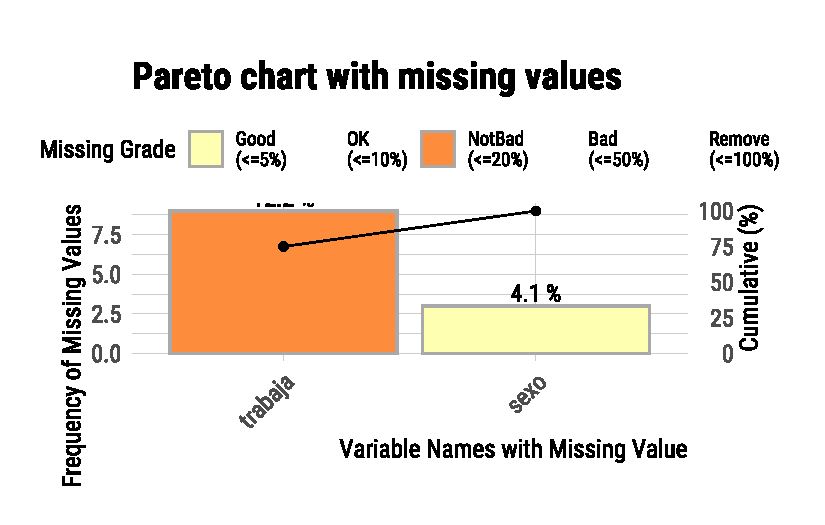
\includegraphics[width=0.85\linewidth,height=\textheight,keepaspectratio]{unidad_1/04_analisis_exploratorio_files/figure-pdf/unnamed-chunk-7-1.pdf}
\end{center}

Finalmente, para un diagnóstico más integral de la calidad de las
variables, puede utilizarse la función \texttt{diagnose()}:

\begin{Shaded}
\begin{Highlighting}[]
\FunctionTok{diagnose}\NormalTok{(datos)}
\end{Highlighting}
\end{Shaded}

\begin{verbatim}
# A tibble: 7 x 6
  variables types     missing_count missing_percent unique_count unique_rate
  <chr>     <chr>             <int>           <dbl>        <int>       <dbl>
1 id        numeric               0            0              74      1     
2 sexo      character             3            4.05            3      0.0405
3 edad      numeric               0            0              45      0.608 
4 peso      numeric               0            0              56      0.757 
5 talla     numeric               0            0              38      0.514 
6 trabaja   logical               9           12.2             3      0.0405
7 fecha     Date                  0            0              11      0.149 
\end{verbatim}

Esta función ofrece un resumen detallado que incluye el tipo de
variable, la cantidad de valores faltantes, la proporción de valores
únicos, entre otros indicadores de utilidad para la exploración inicial.

\section{Conocer la distribución de las variables de
interés}\label{conocer-la-distribuciuxf3n-de-las-variables-de-interuxe9s}

\subsection{Resumir variables
cuantitativas}\label{resumir-variables-cuantitativas}

La instalación básica de R tiene incorporadas múltiples funciones
estadísticas que permiten calcular medidas resumen para variables
cuantitativas. Estas funciones pueden integrarse a la función
\texttt{summarise()} de \texttt{tidyverse}.

\subsubsection{Medidas de tendencia
central}\label{medidas-de-tendencia-central}

Las medidas de tendencia central forman parte del grupo de medidas de
posición o localización, pero su objetivo principal es resumir la
información en torno a un valor que representa el ``centro'' de la
distribución. Es decir, un valor respecto al cual tienden a agruparse
los demás valores.

Podemos obtener la media y la mediana de nuestros datos con el siguiente
código:

\begin{Shaded}
\begin{Highlighting}[]
\NormalTok{datos }\SpecialCharTok{|\textgreater{}}
  \FunctionTok{summarise}\NormalTok{(}
    \CommentTok{\# Media}
    \AttributeTok{media =} \FunctionTok{mean}\NormalTok{(edad),}
    \CommentTok{\# Mediana}
    \AttributeTok{mediana =} \FunctionTok{median}\NormalTok{(edad)}
\NormalTok{  )}
\end{Highlighting}
\end{Shaded}

\begin{verbatim}
# A tibble: 1 x 2
  media mediana
  <dbl>   <dbl>
1  48.1    52.5
\end{verbatim}

En cambio, R base no incluye una función específica para calcular la
\textbf{moda}. Para obtenerla, debemos escribir una función propia o
utilizar algún paquete adicional que la implemente (por ejemplo,
\texttt{modeest::mlv()}).

\subsubsection{Medidas de posición}\label{medidas-de-posiciuxf3n}

Las medidas de posición dividen los datos en grupos con igual número de
observaciones. Entre las más utilizadas se encuentran los
\textbf{cuartiles} y \textbf{percentiles}.

La función \texttt{quantile()} del paquete base \texttt{stats} permite
calcular cuartiles u otros percentiles. Por ejemplo, para calcular los
cuartiles Q1 y Q3, indicamos en el argumento \texttt{probs} los valores
0.25 y 0.75:

\begin{Shaded}
\begin{Highlighting}[]
\NormalTok{datos }\SpecialCharTok{|\textgreater{}}
  \FunctionTok{summarise}\NormalTok{(}
    \CommentTok{\# Primer cuartil}
    \AttributeTok{cuartil1 =} \FunctionTok{quantile}\NormalTok{(edad, }\AttributeTok{probs =} \FloatTok{0.25}\NormalTok{),}
    \CommentTok{\# Tercer cuartil}
    \AttributeTok{cuartil3 =} \FunctionTok{quantile}\NormalTok{(edad, }\AttributeTok{probs =} \FloatTok{0.75}\NormalTok{)}
\NormalTok{  )}
\end{Highlighting}
\end{Shaded}

\begin{verbatim}
# A tibble: 1 x 2
  cuartil1 cuartil3
     <dbl>    <dbl>
1       28       64
\end{verbatim}

Para obtener el mínimo y máximo de estos valores numéricos usamos el
siguiente código:

\begin{Shaded}
\begin{Highlighting}[]
\NormalTok{datos }\SpecialCharTok{|\textgreater{}}
  \FunctionTok{summarise}\NormalTok{(}
    \CommentTok{\# Mínimo}
    \AttributeTok{minimo =} \FunctionTok{min}\NormalTok{(edad),}
    \CommentTok{\# Máximo}
    \AttributeTok{maximo =} \FunctionTok{max}\NormalTok{(edad)}
\NormalTok{  )}
\end{Highlighting}
\end{Shaded}

\begin{verbatim}
# A tibble: 1 x 2
  minimo maximo
   <dbl>  <dbl>
1     13     86
\end{verbatim}

\subsubsection{Medidas de dispersión}\label{medidas-de-dispersiuxf3n}

Las medidas de dispersión nos permiten conocer cuán dispersos o
variables son los valores dentro del conjunto de datos.

Entre las más clásicas se encuentran la \textbf{varianza} y el
\textbf{desvío estándar}, que se calculan fácilmente con las funciones
\texttt{var()} y \texttt{sd()}:

\begin{Shaded}
\begin{Highlighting}[]
\NormalTok{datos }\SpecialCharTok{|\textgreater{}}
  \FunctionTok{summarise}\NormalTok{(}
    \CommentTok{\# Varianza}
    \AttributeTok{varianza =} \FunctionTok{var}\NormalTok{(edad),}
    \CommentTok{\# Desvío estándar}
    \AttributeTok{desvio =} \FunctionTok{sd}\NormalTok{(edad)}
\NormalTok{  )}
\end{Highlighting}
\end{Shaded}

\begin{verbatim}
# A tibble: 1 x 2
  varianza desvio
     <dbl>  <dbl>
1     405.   20.1
\end{verbatim}

También puede ser útil calcular el \textbf{rango}, que se obtiene como
la diferencia entre el valor máximo y el mínimo, y el \textbf{rango
intercuartílico (RIC)}, mediante \texttt{IQR()}:

\begin{Shaded}
\begin{Highlighting}[]
\NormalTok{datos }\SpecialCharTok{|\textgreater{}}
  \FunctionTok{summarise}\NormalTok{(}
    \CommentTok{\# Rango}
    \AttributeTok{rango =} \FunctionTok{max}\NormalTok{(edad) }\SpecialCharTok{{-}} \FunctionTok{min}\NormalTok{(edad),}
    \CommentTok{\# Rango intercuartílico}
    \AttributeTok{ric =} \FunctionTok{IQR}\NormalTok{(edad)}
\NormalTok{  )}
\end{Highlighting}
\end{Shaded}

\begin{verbatim}
# A tibble: 1 x 2
  rango   ric
  <dbl> <dbl>
1    73    36
\end{verbatim}

El paquete \texttt{dlookr} ofrece la función \texttt{describe()} para
generar un resumen completo de las variables numéricas:

\begin{Shaded}
\begin{Highlighting}[]
\FunctionTok{describe}\NormalTok{(datos, }\SpecialCharTok{{-}}\NormalTok{id)}
\end{Highlighting}
\end{Shaded}

\begin{verbatim}
# A tibble: 3 x 26
  described_variables     n    na  mean    sd se_mean   IQR skewness kurtosis
  <chr>               <int> <int> <dbl> <dbl>   <dbl> <dbl>    <dbl>    <dbl>
1 edad                   74     0  48.1  20.1    2.34  36     -0.211    -1.11
2 peso                   74     0 358.  323.    37.6  626.     0.451    -1.41
3 talla                  74     0 363.  505.    58.7   12.8    2.19      2.90
# i 17 more variables: p00 <dbl>, p01 <dbl>, p05 <dbl>, p10 <dbl>, p20 <dbl>,
#   p25 <dbl>, p30 <dbl>, p40 <dbl>, p50 <dbl>, p60 <dbl>, p70 <dbl>,
#   p75 <dbl>, p80 <dbl>, p90 <dbl>, p95 <dbl>, p99 <dbl>, p100 <dbl>
\end{verbatim}

Esta función puede aplicarse directamente sobre todo el conjunto de
datos. Si bien selecciona automáticamente las variables numéricas, en
este caso estamos excluyendo explícitamente la variable \texttt{id}, ya
que un identificador no tiene interés estadístico.

El resumen que devuelve incluye:

\begin{itemize}
\item
  \texttt{na}: cantidad de observaciones con datos y con \texttt{NA.}
\item
  \texttt{mean}: media aritmética.
\item
  \texttt{sd}: desvío estándar de la media.
\item
  \texttt{se\_mean}: error estándar de la media.
\item
  \texttt{IQR}: rango intercuartílico.
\item
  Medidas de forma como la simetría (\texttt{skewness}) y la curtosis
  (\texttt{kurtosis}).
\item
  Percentiles, incluyendo la mediana (\texttt{P50}) y los cuartiles
  (\texttt{P25} y \texttt{P75}).
\end{itemize}

\subsection{Resumir variables
cualitativas}\label{resumir-variables-cualitativas}

Las variables cualitativas o categóricas pueden encontrarse en R bajo
los tipos de dato \texttt{character} o \texttt{factor}. En ocasiones
será necesario convertirlas a \texttt{factor}, ya que este tipo permite
aplicar ciertos procedimientos específicos para variables categóricas.

\subsubsection{Frecuencias}\label{frecuencias}

Podemos resumir individualmente variables cualitativas mediante las
frecuencias absolutas y relativas de sus categorías. La función
\texttt{count()} de \texttt{dplyr} nos muestra el conteo absoluto:

\begin{Shaded}
\begin{Highlighting}[]
\NormalTok{datos }\SpecialCharTok{|\textgreater{}}
  \FunctionTok{count}\NormalTok{(sexo)}
\end{Highlighting}
\end{Shaded}

\begin{verbatim}
# A tibble: 3 x 2
  sexo      n
  <chr> <int>
1 F        27
2 M        44
3 <NA>      3
\end{verbatim}

En la salida se incluirán, además de las categorías presentes, las
observaciones con valores faltantes (\texttt{NA}).

La inclusión o no de los valores faltantes dependerá del propósito del
análisis. Para excluirlos, podemos utilizar \texttt{drop\_na()}:

\begin{Shaded}
\begin{Highlighting}[]
\NormalTok{datos }\SpecialCharTok{|\textgreater{}}
  \FunctionTok{count}\NormalTok{(sexo) }\SpecialCharTok{|\textgreater{}}
  \CommentTok{\# Saltea los valores NA}
  \FunctionTok{drop\_na}\NormalTok{()}
\end{Highlighting}
\end{Shaded}

\begin{verbatim}
# A tibble: 2 x 2
  sexo      n
  <chr> <int>
1 F        27
2 M        44
\end{verbatim}

Para obtener frecuencias relativas en porcentaje:

\begin{Shaded}
\begin{Highlighting}[]
\NormalTok{datos }\SpecialCharTok{|\textgreater{}}
  \FunctionTok{count}\NormalTok{(sexo) }\SpecialCharTok{|\textgreater{}}
  \CommentTok{\# Saltea los valores NA}
  \FunctionTok{drop\_na}\NormalTok{() }\SpecialCharTok{|\textgreater{}}
  \CommentTok{\# Transforma a porcentajes}
  \FunctionTok{mutate}\NormalTok{(}\AttributeTok{porc =} \DecValTok{100} \SpecialCharTok{*}\NormalTok{ n }\SpecialCharTok{/} \FunctionTok{sum}\NormalTok{(n))}
\end{Highlighting}
\end{Shaded}

\begin{verbatim}
# A tibble: 2 x 3
  sexo      n  porc
  <chr> <int> <dbl>
1 F        27  38.0
2 M        44  62.0
\end{verbatim}

Redondeamos el valor del porcentaje con \texttt{round()}:

\begin{Shaded}
\begin{Highlighting}[]
\NormalTok{datos }\SpecialCharTok{|\textgreater{}}
  \FunctionTok{count}\NormalTok{(sexo) }\SpecialCharTok{|\textgreater{}}
  \CommentTok{\# Saltea los valores NA}
  \FunctionTok{drop\_na}\NormalTok{() }\SpecialCharTok{|\textgreater{}}
  \CommentTok{\# Transforma a porcentajes y redondea decimales}
  \FunctionTok{mutate}\NormalTok{(}
    \AttributeTok{porc =} \DecValTok{100} \SpecialCharTok{*}\NormalTok{ n }\SpecialCharTok{/} \FunctionTok{sum}\NormalTok{(n),}
    \AttributeTok{porc =} \FunctionTok{round}\NormalTok{(porc, }\AttributeTok{digits =} \DecValTok{2}\NormalTok{)}
\NormalTok{  )}
\end{Highlighting}
\end{Shaded}

\begin{verbatim}
# A tibble: 2 x 3
  sexo      n  porc
  <chr> <int> <dbl>
1 F        27  38.0
2 M        44  62.0
\end{verbatim}

El paquete \texttt{janitor} {[}@janitor{]} ofrece una alternativa más
completa mediante la función \texttt{tabyl()}:

\begin{Shaded}
\begin{Highlighting}[]
\NormalTok{datos }\SpecialCharTok{|\textgreater{}}
  \FunctionTok{tabyl}\NormalTok{(sexo)}
\end{Highlighting}
\end{Shaded}

\begin{verbatim}
 sexo  n    percent valid_percent
    F 27 0.36486486     0.3802817
    M 44 0.59459459     0.6197183
 <NA>  3 0.04054054            NA
\end{verbatim}

Esta función muestra tanto frecuencias absolutas como relativas,
incluyendo y excluyendo los valores \texttt{NA} (porcentaje sobre el
total de valores válidos).

Podemos mejorar la presentación combinando otras funciones del paquete:

\begin{Shaded}
\begin{Highlighting}[]
\NormalTok{datos }\SpecialCharTok{|\textgreater{}}
  \CommentTok{\# Excluímos valores NA}
  \FunctionTok{tabyl}\NormalTok{(sexo, }\AttributeTok{show\_na =}\NormalTok{ F) }\SpecialCharTok{|\textgreater{}}
  \CommentTok{\# Añadimos totales por fila}
  \FunctionTok{adorn\_totals}\NormalTok{(}\AttributeTok{where =} \StringTok{"row"}\NormalTok{) }\SpecialCharTok{|\textgreater{}}
  \CommentTok{\# Redondea porcentajes a 2 decimales}
  \FunctionTok{adorn\_pct\_formatting}\NormalTok{(}\AttributeTok{digits =} \DecValTok{2}\NormalTok{)}
\end{Highlighting}
\end{Shaded}

\begin{verbatim}
  sexo  n percent
     F 27  38.03%
     M 44  61.97%
 Total 71 100.00%
\end{verbatim}

\subsubsection{Tablas de contingencia}\label{tablas-de-contingencia}

La forma más adecuada de describir la relación entre dos variables
cualitativas es a través de una \textbf{tabla de contingencia}, en la
cual:

\begin{itemize}
\item
  Las filas representan las categorías de una variable.
\item
  Las columnas representan las categorías de otra variable.
\item
  Las celdas muestran el número de observaciones correspondientes a cada
  combinación de categorías.
\end{itemize}

La función \texttt{tabyl()} también permite crear este tipo de tablas. A
continuación, un ejemplo entre \texttt{sexo} y \texttt{trabaja} (aunque
\texttt{trabaja} sea lógica, puede tratarse como categórica):

\begin{Shaded}
\begin{Highlighting}[]
\NormalTok{datos }\SpecialCharTok{|\textgreater{}}
  \FunctionTok{tabyl}\NormalTok{(sexo, trabaja)}
\end{Highlighting}
\end{Shaded}

\begin{verbatim}
 sexo FALSE TRUE NA_
    F     8   15   4
    M    17   22   5
 <NA>     1    2   0
\end{verbatim}

Recordemos que el orden dentro de los paréntesis de la función es igual
al de los índices, el primer argumento es la variable que aparecerá en
las filas y el segundo la variable de las columnas. Por ese motivo, en
la tabla de contingencia absoluta tenemos \texttt{sexo} en las filas y
\texttt{trabaja} en las columnas.

Se puede mejorar la tabla excluyendo los valores \texttt{NA} y agregando
totales por fila:

\begin{Shaded}
\begin{Highlighting}[]
\NormalTok{datos }\SpecialCharTok{|\textgreater{}}
  \CommentTok{\# Excluímos valores NA}
  \FunctionTok{tabyl}\NormalTok{(sexo, trabaja, }\AttributeTok{show\_na =}\NormalTok{ F) }\SpecialCharTok{|\textgreater{}}
  \CommentTok{\# Añadimos totales por fila}
  \FunctionTok{adorn\_totals}\NormalTok{(}\AttributeTok{where =} \StringTok{"row"}\NormalTok{)}
\end{Highlighting}
\end{Shaded}

\begin{verbatim}
  sexo FALSE TRUE
     F     8   15
     M    17   22
 Total    25   37
\end{verbatim}

Para calcular frecuencias relativas porcentuales por columna usamos el
siguiente código:

\begin{Shaded}
\begin{Highlighting}[]
\NormalTok{datos }\SpecialCharTok{|\textgreater{}}
  \CommentTok{\# Excluímos valores NA}
  \FunctionTok{tabyl}\NormalTok{(sexo, trabaja, }\AttributeTok{show\_na =}\NormalTok{ F) }\SpecialCharTok{|\textgreater{}}
  \CommentTok{\# Añadimos totales}
  \FunctionTok{adorn\_totals}\NormalTok{(}\AttributeTok{where =} \StringTok{"row"}\NormalTok{) }\SpecialCharTok{|\textgreater{}}
  \CommentTok{\# Añadimos porcentajes por columna}
  \FunctionTok{adorn\_percentages}\NormalTok{(}\AttributeTok{denominator =} \StringTok{"col"}\NormalTok{) }\SpecialCharTok{|\textgreater{}}
  \CommentTok{\# Redondea porcentajes a 2 decimales}
  \FunctionTok{adorn\_pct\_formatting}\NormalTok{(}\AttributeTok{digits =} \DecValTok{2}\NormalTok{)}
\end{Highlighting}
\end{Shaded}

\begin{verbatim}
  sexo   FALSE    TRUE
     F  32.00%  40.54%
     M  68.00%  59.46%
 Total 100.00% 100.00%
\end{verbatim}

Calculamos frecuencias relativas porcentuales por fila:

\begin{Shaded}
\begin{Highlighting}[]
\NormalTok{datos }\SpecialCharTok{|\textgreater{}}
  \CommentTok{\# Excluímos valores NA}
  \FunctionTok{tabyl}\NormalTok{(sexo, trabaja, }\AttributeTok{show\_na =}\NormalTok{ F) }\SpecialCharTok{|\textgreater{}}
  \CommentTok{\# Añadimos totales por columna}
  \FunctionTok{adorn\_totals}\NormalTok{(}\AttributeTok{where =} \StringTok{"col"}\NormalTok{) }\SpecialCharTok{|\textgreater{}}
  \CommentTok{\# Añadimos porcentajes por fila}
  \FunctionTok{adorn\_percentages}\NormalTok{(}\AttributeTok{denominator =} \StringTok{"row"}\NormalTok{) }\SpecialCharTok{|\textgreater{}}
  \CommentTok{\# Redondea porcentajes a 2 decimales}
  \FunctionTok{adorn\_pct\_formatting}\NormalTok{(}\AttributeTok{digits =} \DecValTok{2}\NormalTok{)}
\end{Highlighting}
\end{Shaded}

\begin{verbatim}
 sexo  FALSE   TRUE   Total
    F 34.78% 65.22% 100.00%
    M 43.59% 56.41% 100.00%
\end{verbatim}

Cambiando el argumento \texttt{denominator} por \texttt{"all"} se
calculan frecuencias relativas al total:

\begin{Shaded}
\begin{Highlighting}[]
\NormalTok{datos }\SpecialCharTok{|\textgreater{}}
  \CommentTok{\# Excluímos valores NA}
  \FunctionTok{tabyl}\NormalTok{(sexo, trabaja, }\AttributeTok{show\_na =}\NormalTok{ F) }\SpecialCharTok{|\textgreater{}}
  \CommentTok{\# Añadimos totales por columna}
  \FunctionTok{adorn\_totals}\NormalTok{(}\AttributeTok{where =} \StringTok{"col"}\NormalTok{) }\SpecialCharTok{|\textgreater{}}
  \CommentTok{\# Añadimos porcentajes al total}
  \FunctionTok{adorn\_percentages}\NormalTok{(}\AttributeTok{denominator =} \StringTok{"all"}\NormalTok{) }\SpecialCharTok{|\textgreater{}}
  \CommentTok{\# Redondea porcentajes a 2 decimales}
  \FunctionTok{adorn\_pct\_formatting}\NormalTok{(}\AttributeTok{digits =} \DecValTok{2}\NormalTok{)}
\end{Highlighting}
\end{Shaded}

\begin{verbatim}
 sexo  FALSE   TRUE  Total
    F 12.90% 24.19% 37.10%
    M 27.42% 35.48% 62.90%
\end{verbatim}

\subsection{Explorar variables mediante
gráficos}\label{explorar-variables-mediante-gruxe1ficos}

Uno de los aportes más importantes de John Tukey al análisis de datos es
la incorporación de los gráficos como herramienta exploratoria. A través
de representaciones visuales podemos detectar rápidamente patrones,
anomalías, valores extremos, asimetrías o relaciones entre variables.

En R, los gráficos más útiles para explorar la distribución
\textbf{univariada} de las variables son:

\begin{itemize}
\item
  Para variables \textbf{cualitativas}: gráficos de barras
\item
  Para variables \textbf{cuantitativas}: histogramas, gráficos de
  densidad, boxplots y violin plots
\item
  Cuando queremos explorar la relación entre \textbf{dos o más
  variables}, los tipos de gráficos más comunes incluyen:

  \begin{itemize}
  \item
    Diagramas de dispersión (puntos)
  \item
    Gráficos de líneas
  \item
    Gráficos de mosaico para variables categóricas cruzadas
  \end{itemize}
\end{itemize}

El lenguaje R soporta una serie de sistemas gráficos asociados a
paquetes como \texttt{graphics}, \texttt{lattice}, \texttt{ggplot2},
etc. que sirven de base incluso para otros paquetes con funciones más
específicas. Actualmente el estándar gráfico en R es \texttt{ggplot2}.

En el documento dedicado a
\hyperref[gruxe1ficos-estaduxedsticos-con-ggplot2]{\textbf{tidyverse}}
ya explicamos cómo funciona \texttt{ggplot2}. Aquí nos concentraremos
únicamente en aplicar distintos elementos geométricos (\texttt{geoms})
para representar las variables según su tipo.

\subsubsection{Barras (univariado)}\label{barras-univariado}

El gráfico de barras permite visualizar la frecuencia de las categorías
de una variable cualitativa:

\begin{Shaded}
\begin{Highlighting}[]
\NormalTok{datos }\SpecialCharTok{|\textgreater{}}
  \CommentTok{\# Omitimos los NA de sexo}
  \FunctionTok{drop\_na}\NormalTok{(sexo) }\SpecialCharTok{|\textgreater{}}
  \CommentTok{\# Generamos histograma}
  \FunctionTok{ggplot}\NormalTok{(}\FunctionTok{aes}\NormalTok{(}\AttributeTok{x =}\NormalTok{ sexo, }\AttributeTok{fill =}\NormalTok{ sexo)) }\SpecialCharTok{+}
  \FunctionTok{geom\_bar}\NormalTok{() }\SpecialCharTok{+}
  \FunctionTok{scale\_fill\_manual}\NormalTok{(}\AttributeTok{values =} \FunctionTok{c}\NormalTok{(}\StringTok{"palevioletred4"}\NormalTok{, }\StringTok{"orange"}\NormalTok{)) }\SpecialCharTok{+}
  \FunctionTok{theme\_minimal}\NormalTok{()}
\end{Highlighting}
\end{Shaded}

\begin{center}
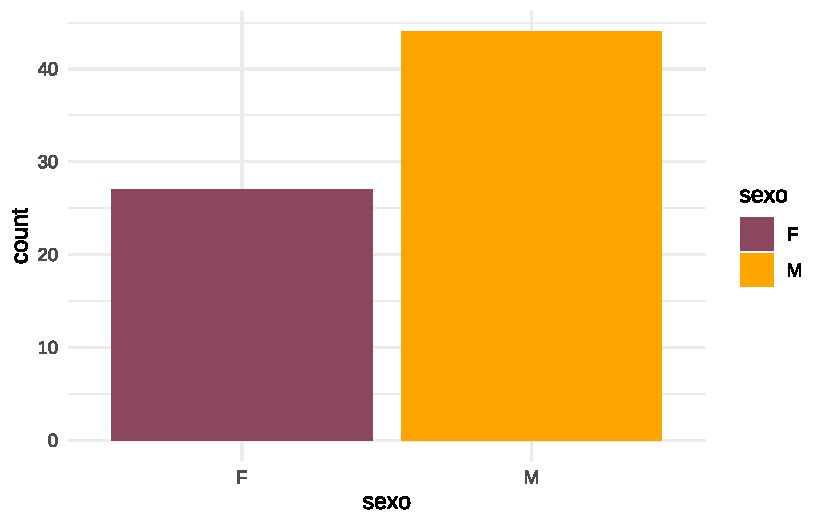
\includegraphics[width=0.85\linewidth,height=\textheight,keepaspectratio]{unidad_1/04_analisis_exploratorio_files/figure-pdf/unnamed-chunk-26-1.pdf}
\end{center}

\subsubsection{Barras (bivariado)}\label{barras-bivariado}

Cuando cruzamos dos variables categóricas, podemos representar la
relación entre ambas modificando el argumento \texttt{position} de
\texttt{geom\_bar()}.

El argumento \texttt{position\ =\ "stack"} nos muestra los valores
absolutos acumulados:

\begin{Shaded}
\begin{Highlighting}[]
\NormalTok{datos }\SpecialCharTok{|\textgreater{}}
  \CommentTok{\# Omitimos los NA de sexo y trabaja}
  \FunctionTok{drop\_na}\NormalTok{(sexo, trabaja) }\SpecialCharTok{|\textgreater{}}
  \CommentTok{\# Generamos gráfico de barras}
  \FunctionTok{ggplot}\NormalTok{(}\FunctionTok{aes}\NormalTok{(}\AttributeTok{x =}\NormalTok{ sexo, }\AttributeTok{fill =}\NormalTok{ trabaja)) }\SpecialCharTok{+}
  \FunctionTok{geom\_bar}\NormalTok{(}\AttributeTok{position =} \StringTok{"stack"}\NormalTok{) }\SpecialCharTok{+}
  \FunctionTok{scale\_fill\_brewer}\NormalTok{(}\AttributeTok{palette =} \StringTok{"Set1"}\NormalTok{) }\SpecialCharTok{+}
  \FunctionTok{theme\_minimal}\NormalTok{()}
\end{Highlighting}
\end{Shaded}

\begin{center}
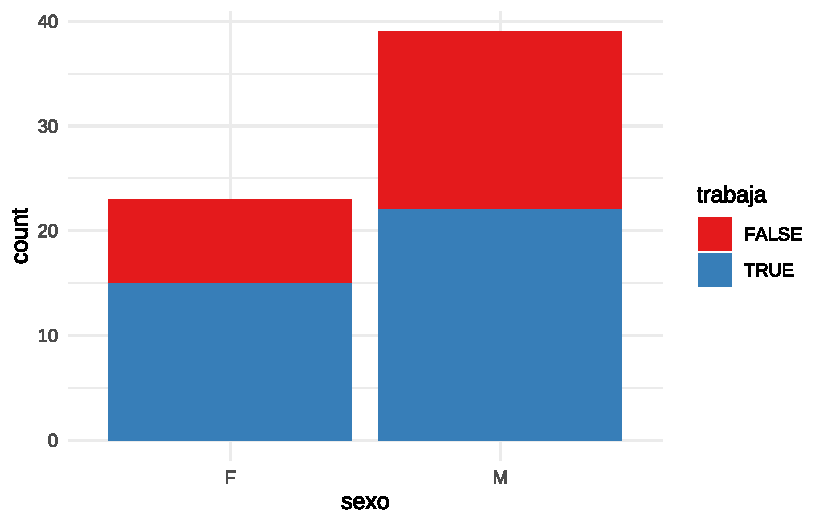
\includegraphics[width=0.85\linewidth,height=\textheight,keepaspectratio]{unidad_1/04_analisis_exploratorio_files/figure-pdf/unnamed-chunk-27-1.pdf}
\end{center}

Por otro lado, el argumento \texttt{position\ =\ "dodge"} muestra las
barras lado a lado, permitiendo comparar proporciones entre grupos:

\begin{Shaded}
\begin{Highlighting}[]
\NormalTok{datos }\SpecialCharTok{|\textgreater{}}
  \CommentTok{\# Omitimos los NA de sexo y trabaja}
  \FunctionTok{drop\_na}\NormalTok{(sexo, trabaja) }\SpecialCharTok{|\textgreater{}}
  \CommentTok{\# Generamos gráfico de barras}
  \FunctionTok{ggplot}\NormalTok{(}\FunctionTok{aes}\NormalTok{(}\AttributeTok{x =}\NormalTok{ sexo, }\AttributeTok{fill =}\NormalTok{ trabaja)) }\SpecialCharTok{+}
  \FunctionTok{geom\_bar}\NormalTok{(}\AttributeTok{position =} \StringTok{"dodge"}\NormalTok{) }\SpecialCharTok{+}
  \FunctionTok{scale\_fill\_brewer}\NormalTok{(}\AttributeTok{palette =} \StringTok{"Set1"}\NormalTok{) }\SpecialCharTok{+}
  \FunctionTok{theme\_minimal}\NormalTok{()}
\end{Highlighting}
\end{Shaded}

\begin{center}
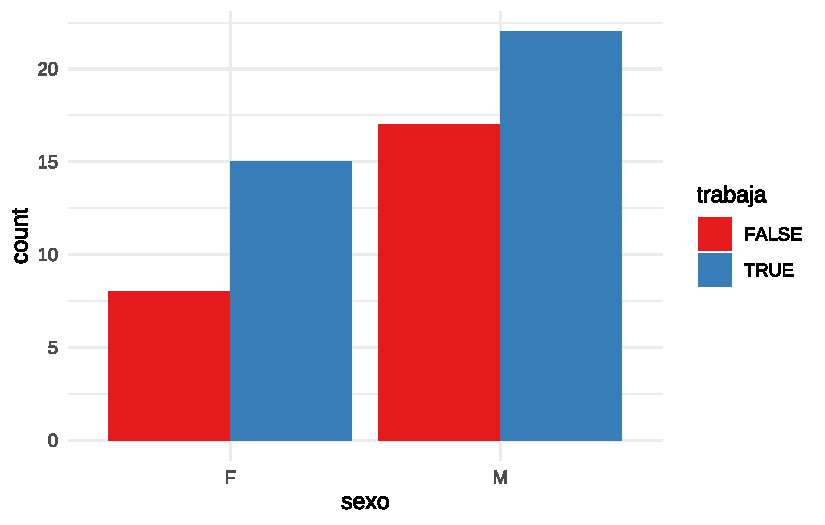
\includegraphics[width=0.85\linewidth,height=\textheight,keepaspectratio]{unidad_1/04_analisis_exploratorio_files/figure-pdf/unnamed-chunk-28-1.pdf}
\end{center}

Finalmente, \texttt{position\ =\ "fill"} convierte las alturas en
proporciones sobre el total por grupo:

\begin{Shaded}
\begin{Highlighting}[]
\NormalTok{datos }\SpecialCharTok{|\textgreater{}}
  \CommentTok{\# Omitimos los NA de sexo y trabaja}
  \FunctionTok{drop\_na}\NormalTok{(sexo, trabaja) }\SpecialCharTok{|\textgreater{}}
  \CommentTok{\# Generamos gráfico de barras}
  \FunctionTok{ggplot}\NormalTok{(}\FunctionTok{aes}\NormalTok{(}\AttributeTok{x =}\NormalTok{ sexo, }\AttributeTok{fill =}\NormalTok{ trabaja)) }\SpecialCharTok{+}
  \FunctionTok{geom\_bar}\NormalTok{(}\AttributeTok{position =} \StringTok{"fill"}\NormalTok{) }\SpecialCharTok{+}
  \FunctionTok{scale\_fill\_brewer}\NormalTok{(}\AttributeTok{palette =} \StringTok{"Set1"}\NormalTok{) }\SpecialCharTok{+}
  \FunctionTok{theme\_minimal}\NormalTok{()}
\end{Highlighting}
\end{Shaded}

\begin{center}
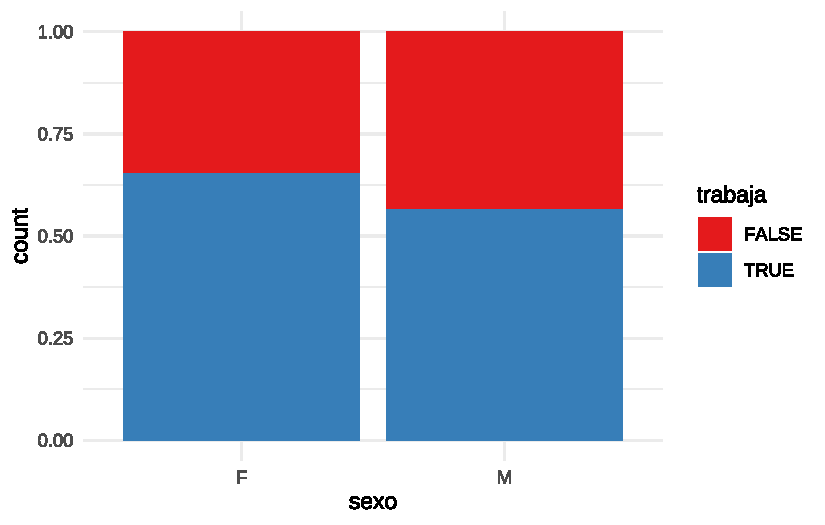
\includegraphics[width=0.85\linewidth,height=\textheight,keepaspectratio]{unidad_1/04_analisis_exploratorio_files/figure-pdf/unnamed-chunk-29-1.pdf}
\end{center}

\subsubsection{Histograma}\label{histograma}

Representa la frecuencia de valores en intervalos definidos. Útil para
observar la forma general de la distribución:

\begin{Shaded}
\begin{Highlighting}[]
\NormalTok{datos }\SpecialCharTok{|\textgreater{}}
  \CommentTok{\# Genera histograma}
  \FunctionTok{ggplot}\NormalTok{(}\FunctionTok{aes}\NormalTok{(}\AttributeTok{x =}\NormalTok{ edad)) }\SpecialCharTok{+}
  \FunctionTok{geom\_histogram}\NormalTok{(}\AttributeTok{binwidth =} \DecValTok{10}\NormalTok{, }\AttributeTok{fill =} \StringTok{"royalblue1"}\NormalTok{, }\AttributeTok{color =} \StringTok{"white"}\NormalTok{)}
\end{Highlighting}
\end{Shaded}

\begin{center}
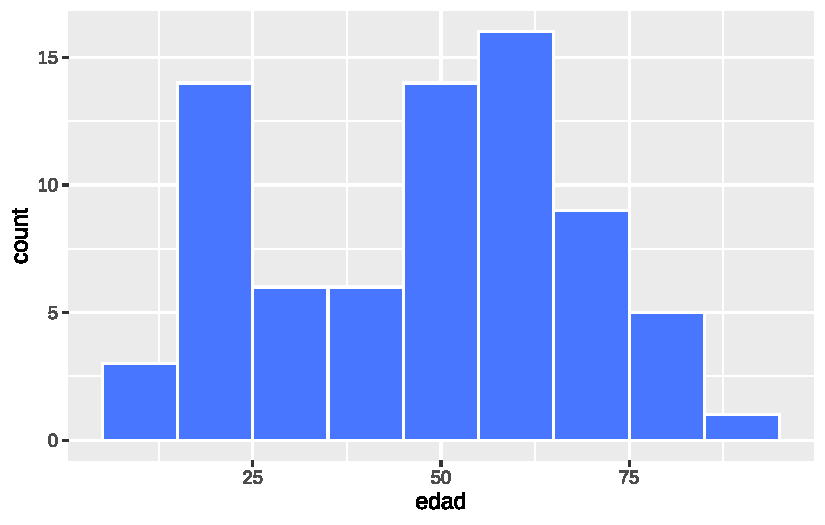
\includegraphics[width=0.85\linewidth,height=\textheight,keepaspectratio]{unidad_1/04_analisis_exploratorio_files/figure-pdf/unnamed-chunk-30-1.pdf}
\end{center}

\subsubsection{Densidad}\label{densidad}

Es una estimación suave de la distribución de frecuencias:

\begin{Shaded}
\begin{Highlighting}[]
\NormalTok{datos }\SpecialCharTok{|\textgreater{}}
  \FunctionTok{ggplot}\NormalTok{(}\FunctionTok{aes}\NormalTok{(}\AttributeTok{x =}\NormalTok{ edad)) }\SpecialCharTok{+}
  \FunctionTok{geom\_density}\NormalTok{(}\AttributeTok{fill =} \StringTok{"thistle1"}\NormalTok{)}
\end{Highlighting}
\end{Shaded}

\begin{center}
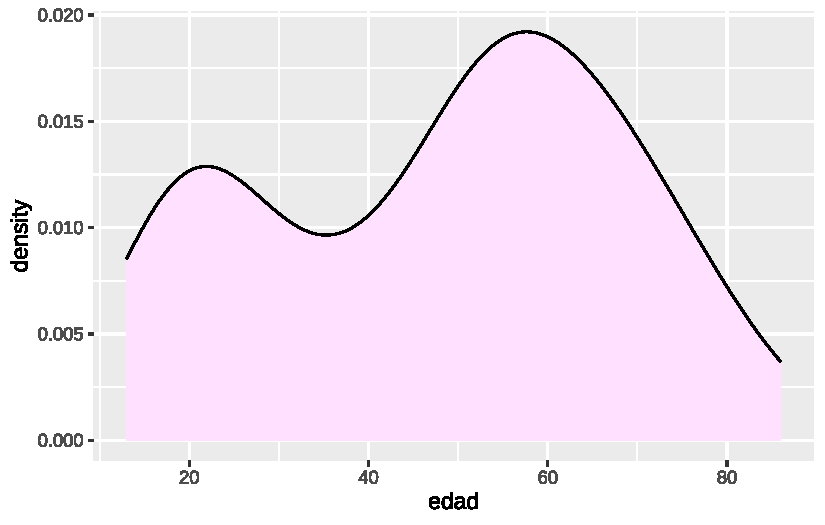
\includegraphics[width=0.85\linewidth,height=\textheight,keepaspectratio]{unidad_1/04_analisis_exploratorio_files/figure-pdf/unnamed-chunk-31-1.pdf}
\end{center}

\subsubsection{\texorpdfstring{\emph{Boxplot}}{Boxplot}}\label{boxplot}

Muestra el rango intercuartílico, la mediana y los valores atípicos.
Ideal para detectar asimetrías y \emph{outliers}:

\begin{Shaded}
\begin{Highlighting}[]
\NormalTok{datos }\SpecialCharTok{|\textgreater{}}
  \CommentTok{\# Genera boxplot}
  \FunctionTok{ggplot}\NormalTok{(}\FunctionTok{aes}\NormalTok{(}\AttributeTok{x =}\NormalTok{ edad)) }\SpecialCharTok{+}
  \FunctionTok{geom\_boxplot}\NormalTok{(}\AttributeTok{fill =} \StringTok{"seagreen4"}\NormalTok{)}
\end{Highlighting}
\end{Shaded}

\begin{center}
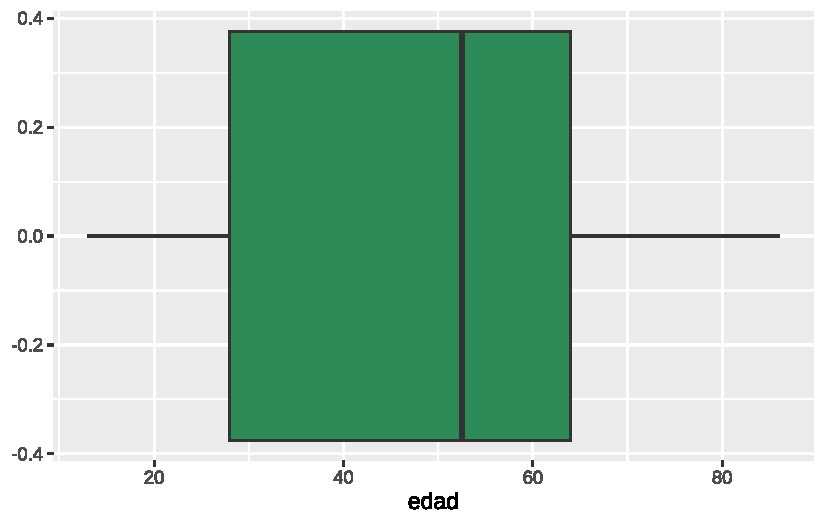
\includegraphics[width=0.85\linewidth,height=\textheight,keepaspectratio]{unidad_1/04_analisis_exploratorio_files/figure-pdf/unnamed-chunk-32-1.pdf}
\end{center}

\subsubsection{\texorpdfstring{\emph{Violinplot}}{Violinplot}}\label{violinplot}

Combina el \emph{boxplot} con una curva de densidad reflejada. Permite
visualizar tanto la forma de la distribución como los cuantiles:

\begin{Shaded}
\begin{Highlighting}[]
\NormalTok{datos }\SpecialCharTok{|\textgreater{}}
  \CommentTok{\# Omitimos los NA de sexo}
  \FunctionTok{drop\_na}\NormalTok{(sexo) }\SpecialCharTok{|\textgreater{}}
  \CommentTok{\# Genera violinplot}
  \FunctionTok{ggplot}\NormalTok{(}\FunctionTok{aes}\NormalTok{(}\AttributeTok{x =}\NormalTok{ edad, }\AttributeTok{y =}\NormalTok{ sexo, }\AttributeTok{fill =}\NormalTok{ sexo)) }\SpecialCharTok{+}
  \FunctionTok{geom\_violin}\NormalTok{() }\SpecialCharTok{+}
  \FunctionTok{scale\_fill\_brewer}\NormalTok{(}\AttributeTok{palette =} \StringTok{"Set2"}\NormalTok{) }\SpecialCharTok{+}
  \FunctionTok{theme\_light}\NormalTok{()}
\end{Highlighting}
\end{Shaded}

\begin{center}
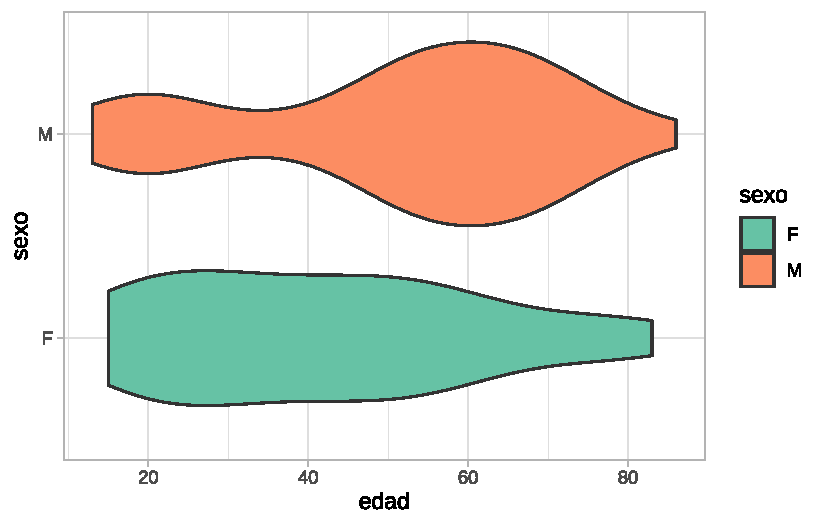
\includegraphics[width=0.85\linewidth,height=\textheight,keepaspectratio]{unidad_1/04_analisis_exploratorio_files/figure-pdf/unnamed-chunk-33-1.pdf}
\end{center}

\textbf{\emph{Q-Q Plot}}

Los gráficos Q-Q (cuantil-cuantil) permiten evaluar visualmente si una
variable sigue una distribución teórica, como la normal. Suelen usarse
como método gráfico para analizar ``normalidad'', es decir cuanto se
asemeja la distribución de la variable a la distribución normal o
gaussiana.

La función \texttt{plot\_normality()} de \texttt{dlookr} muestra un
diagnóstico gráfico de normalidad de una variable usando histogramas y
Q-Q plot. Además muestra otros histogramas con conversiones de datos
(logarítmico y raíz cuadrada por defecto, pero también ``Box-Cox'' y
otras):

\begin{Shaded}
\begin{Highlighting}[]
\CommentTok{\# Sobre la variable edad}
\NormalTok{datos }\SpecialCharTok{|\textgreater{}}
  \FunctionTok{plot\_normality}\NormalTok{(edad)}
\end{Highlighting}
\end{Shaded}

\begin{center}
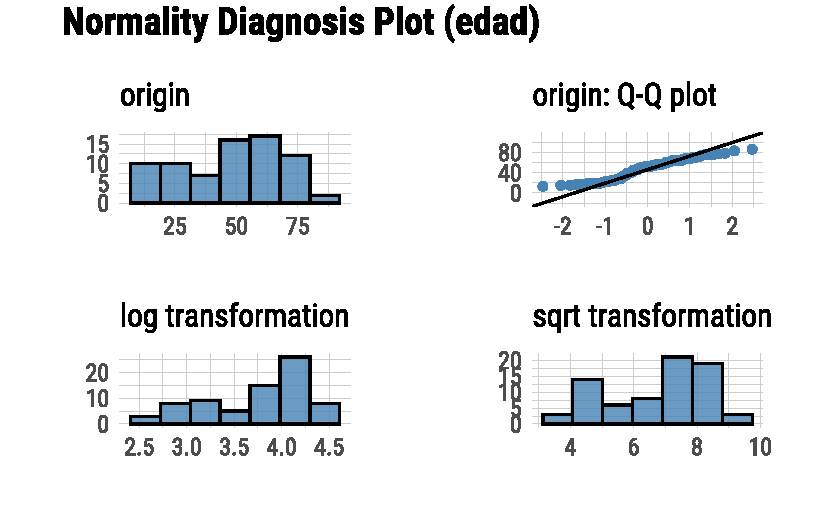
\includegraphics[width=0.85\linewidth,height=\textheight,keepaspectratio]{unidad_1/04_analisis_exploratorio_files/figure-pdf/unnamed-chunk-34-1.pdf}
\end{center}

\begin{Shaded}
\begin{Highlighting}[]
\CommentTok{\# Sobre la variable peso}
\NormalTok{datos }\SpecialCharTok{|\textgreater{}}
  \FunctionTok{plot\_normality}\NormalTok{(peso)}
\end{Highlighting}
\end{Shaded}

\begin{center}
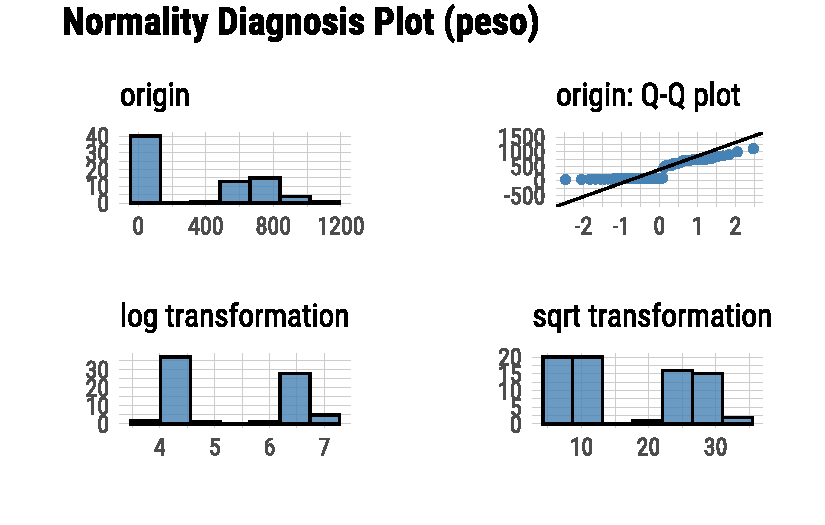
\includegraphics[width=0.85\linewidth,height=\textheight,keepaspectratio]{unidad_1/04_analisis_exploratorio_files/figure-pdf/unnamed-chunk-34-2.pdf}
\end{center}

Podemos decir que la variable \texttt{peso} se ajusta mejor a una
distribución normal, ya que los puntos del Q-Q plot se alinean más
cercanamente a la diagonal teórica.

\begin{quote}
\textbf{Nota}: Este análisis gráfico de normalidad suele complementarse
con pruebas estadísticas específicas, que abordaremos en la próxima
unidad.
\end{quote}

\section{Detección de valores
atípicos}\label{detecciuxf3n-de-valores-atuxedpicos}

Un valor atípico (\emph{outlier}) es una observación que se encuentra
numéricamente alejada del resto de los datos. Su presencia puede tener
diferentes causas, y su tratamiento dependerá del contexto:

\begin{itemize}
\item
  \textbf{Errores de carga o procedimiento}: deben corregirse si se
  detectan.
\item
  \textbf{Valores extremos plausibles}: pueden ser válidos, pero
  conviene evaluarlos en detalle.
\item
  \textbf{Eventos extraordinarios o causas desconocidas}: si no se
  pueden justificar, suelen excluirse del análisis.
\end{itemize}

Estos valores pueden afectar sensiblemente ciertos estadísticos como la
media, distorsionando su interpretación.

Una forma gráfica común de detectar valores atípicos es mediante los
\emph{boxplots}. Los puntos situados fuera de los ``bigotes''
representan posibles \emph{outliers}.

A continuación, se presenta un ejemplo con la variable \texttt{peso},
donde se observa un valor extremo en el límite superior de la
distribución (punto rojo):

\begin{Shaded}
\begin{Highlighting}[]
\NormalTok{datos }\SpecialCharTok{|\textgreater{}}
  \FunctionTok{ggplot}\NormalTok{(}\FunctionTok{aes}\NormalTok{(}\AttributeTok{x =}\NormalTok{ peso)) }\SpecialCharTok{+}
  \FunctionTok{geom\_boxplot}\NormalTok{(}\AttributeTok{fill =} \StringTok{"darkkhaki"}\NormalTok{, }\AttributeTok{outlier.color =} \StringTok{"red"}\NormalTok{)}
\end{Highlighting}
\end{Shaded}

\begin{center}
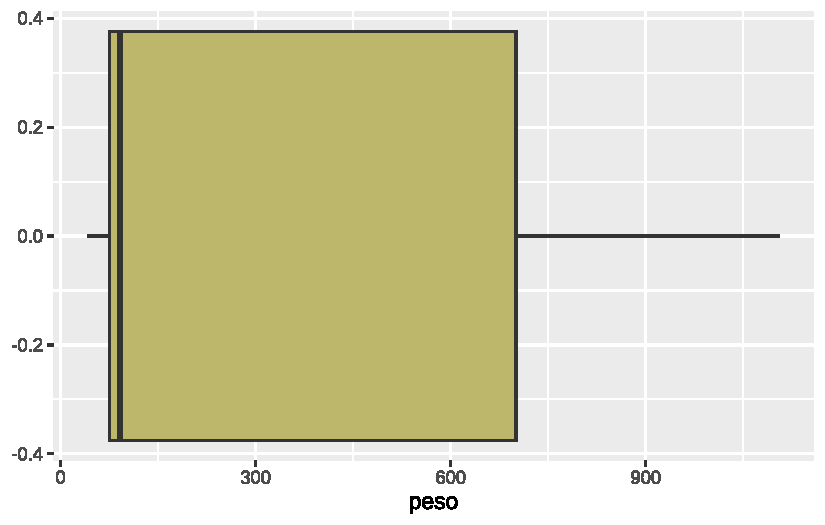
\includegraphics[width=0.85\linewidth,height=\textheight,keepaspectratio]{unidad_1/04_analisis_exploratorio_files/figure-pdf/unnamed-chunk-35-1.pdf}
\end{center}

Este valor coincide con el máximo observado:

\begin{Shaded}
\begin{Highlighting}[]
\FunctionTok{max}\NormalTok{(datos}\SpecialCharTok{$}\NormalTok{peso)}
\end{Highlighting}
\end{Shaded}

\begin{verbatim}
[1] 1105
\end{verbatim}

El paquete \texttt{dlookr} incluye la función
\texttt{diagnose\_outlier()} para la detección automatizada de valores
atípicos en todas las variables numéricas de un conjunto de datos:

\begin{Shaded}
\begin{Highlighting}[]
\FunctionTok{diagnose\_outlier}\NormalTok{(datos)}
\end{Highlighting}
\end{Shaded}

\begin{verbatim}
# A tibble: 4 x 6
  variables outliers_cnt outliers_ratio outliers_mean with_mean without_mean
  <chr>            <int>          <dbl>         <dbl>     <dbl>        <dbl>
1 id                   0            0             NaN      37.5         37.5
2 edad                 0            0             NaN      48.1         48.1
3 peso                 0            0             NaN     358.         358. 
4 talla               10           13.5          1630     363.         165. 
\end{verbatim}

Esta función devuelve una tabla que incluye, para cada variable:
cantidad y proporción de \emph{outliers} detectados, media de la
variable incluyendo los \emph{outliers}, media de la variable excluyendo
los \emph{outliers}. En función de estos dos estadísticos se puede
comparar el efecto de los valores atípicos en la media.

El paquete \texttt{skimr} {[}@skimr{]} permite obtener un resumen
estadístico compacto y amigable de un conjunto de datos mediante la
función \texttt{skim()}:

\begin{Shaded}
\begin{Highlighting}[]
\FunctionTok{skim}\NormalTok{(datos)}
\end{Highlighting}
\end{Shaded}

\begin{longtable}[]{@{}ll@{}}
\caption{Data summary}\tabularnewline
\toprule\noalign{}
\endfirsthead
\endhead
\bottomrule\noalign{}
\endlastfoot
Name & datos \\
Number of rows & 74 \\
Number of columns & 7 \\
\_\_\_\_\_\_\_\_\_\_\_\_\_\_\_\_\_\_\_\_\_\_\_ & \\
Column type frequency: & \\
character & 1 \\
Date & 1 \\
logical & 1 \\
numeric & 4 \\
\_\_\_\_\_\_\_\_\_\_\_\_\_\_\_\_\_\_\_\_\_\_\_\_ & \\
Group variables & None \\
\end{longtable}

\textbf{Variable type: character}

{\def\LTcaptype{none} % do not increment counter
\begin{longtable}[]{@{}
  >{\raggedright\arraybackslash}p{(\linewidth - 14\tabcolsep) * \real{0.1944}}
  >{\raggedleft\arraybackslash}p{(\linewidth - 14\tabcolsep) * \real{0.1389}}
  >{\raggedleft\arraybackslash}p{(\linewidth - 14\tabcolsep) * \real{0.1944}}
  >{\raggedleft\arraybackslash}p{(\linewidth - 14\tabcolsep) * \real{0.0556}}
  >{\raggedleft\arraybackslash}p{(\linewidth - 14\tabcolsep) * \real{0.0556}}
  >{\raggedleft\arraybackslash}p{(\linewidth - 14\tabcolsep) * \real{0.0833}}
  >{\raggedleft\arraybackslash}p{(\linewidth - 14\tabcolsep) * \real{0.1250}}
  >{\raggedleft\arraybackslash}p{(\linewidth - 14\tabcolsep) * \real{0.1528}}@{}}
\toprule\noalign{}
\begin{minipage}[b]{\linewidth}\raggedright
skim\_variable
\end{minipage} & \begin{minipage}[b]{\linewidth}\raggedleft
n\_missing
\end{minipage} & \begin{minipage}[b]{\linewidth}\raggedleft
complete\_rate
\end{minipage} & \begin{minipage}[b]{\linewidth}\raggedleft
min
\end{minipage} & \begin{minipage}[b]{\linewidth}\raggedleft
max
\end{minipage} & \begin{minipage}[b]{\linewidth}\raggedleft
empty
\end{minipage} & \begin{minipage}[b]{\linewidth}\raggedleft
n\_unique
\end{minipage} & \begin{minipage}[b]{\linewidth}\raggedleft
whitespace
\end{minipage} \\
\midrule\noalign{}
\endhead
\bottomrule\noalign{}
\endlastfoot
sexo & 3 & 0.96 & 1 & 1 & 0 & 2 & 0 \\
\end{longtable}
}

\textbf{Variable type: Date}

{\def\LTcaptype{none} % do not increment counter
\begin{longtable}[]{@{}
  >{\raggedright\arraybackslash}p{(\linewidth - 12\tabcolsep) * \real{0.1750}}
  >{\raggedleft\arraybackslash}p{(\linewidth - 12\tabcolsep) * \real{0.1250}}
  >{\raggedleft\arraybackslash}p{(\linewidth - 12\tabcolsep) * \real{0.1750}}
  >{\raggedright\arraybackslash}p{(\linewidth - 12\tabcolsep) * \real{0.1375}}
  >{\raggedright\arraybackslash}p{(\linewidth - 12\tabcolsep) * \real{0.1375}}
  >{\raggedright\arraybackslash}p{(\linewidth - 12\tabcolsep) * \real{0.1375}}
  >{\raggedleft\arraybackslash}p{(\linewidth - 12\tabcolsep) * \real{0.1125}}@{}}
\toprule\noalign{}
\begin{minipage}[b]{\linewidth}\raggedright
skim\_variable
\end{minipage} & \begin{minipage}[b]{\linewidth}\raggedleft
n\_missing
\end{minipage} & \begin{minipage}[b]{\linewidth}\raggedleft
complete\_rate
\end{minipage} & \begin{minipage}[b]{\linewidth}\raggedright
min
\end{minipage} & \begin{minipage}[b]{\linewidth}\raggedright
max
\end{minipage} & \begin{minipage}[b]{\linewidth}\raggedright
median
\end{minipage} & \begin{minipage}[b]{\linewidth}\raggedleft
n\_unique
\end{minipage} \\
\midrule\noalign{}
\endhead
\bottomrule\noalign{}
\endlastfoot
fecha & 0 & 1 & 2020-10-20 & 2020-12-15 & 2020-11-11 & 11 \\
\end{longtable}
}

\textbf{Variable type: logical}

{\def\LTcaptype{none} % do not increment counter
\begin{longtable}[]{@{}lrrrl@{}}
\toprule\noalign{}
skim\_variable & n\_missing & complete\_rate & mean & count \\
\midrule\noalign{}
\endhead
\bottomrule\noalign{}
\endlastfoot
trabaja & 9 & 0.88 & 0.6 & TRU: 39, FAL: 26 \\
\end{longtable}
}

\textbf{Variable type: numeric}

{\def\LTcaptype{none} % do not increment counter
\begin{longtable}[]{@{}
  >{\raggedright\arraybackslash}p{(\linewidth - 20\tabcolsep) * \real{0.1609}}
  >{\raggedleft\arraybackslash}p{(\linewidth - 20\tabcolsep) * \real{0.1149}}
  >{\raggedleft\arraybackslash}p{(\linewidth - 20\tabcolsep) * \real{0.1609}}
  >{\raggedleft\arraybackslash}p{(\linewidth - 20\tabcolsep) * \real{0.0805}}
  >{\raggedleft\arraybackslash}p{(\linewidth - 20\tabcolsep) * \real{0.0805}}
  >{\raggedleft\arraybackslash}p{(\linewidth - 20\tabcolsep) * \real{0.0460}}
  >{\raggedleft\arraybackslash}p{(\linewidth - 20\tabcolsep) * \real{0.0805}}
  >{\raggedleft\arraybackslash}p{(\linewidth - 20\tabcolsep) * \real{0.0690}}
  >{\raggedleft\arraybackslash}p{(\linewidth - 20\tabcolsep) * \real{0.0805}}
  >{\raggedleft\arraybackslash}p{(\linewidth - 20\tabcolsep) * \real{0.0575}}
  >{\raggedright\arraybackslash}p{(\linewidth - 20\tabcolsep) * \real{0.0690}}@{}}
\toprule\noalign{}
\begin{minipage}[b]{\linewidth}\raggedright
skim\_variable
\end{minipage} & \begin{minipage}[b]{\linewidth}\raggedleft
n\_missing
\end{minipage} & \begin{minipage}[b]{\linewidth}\raggedleft
complete\_rate
\end{minipage} & \begin{minipage}[b]{\linewidth}\raggedleft
mean
\end{minipage} & \begin{minipage}[b]{\linewidth}\raggedleft
sd
\end{minipage} & \begin{minipage}[b]{\linewidth}\raggedleft
p0
\end{minipage} & \begin{minipage}[b]{\linewidth}\raggedleft
p25
\end{minipage} & \begin{minipage}[b]{\linewidth}\raggedleft
p50
\end{minipage} & \begin{minipage}[b]{\linewidth}\raggedleft
p75
\end{minipage} & \begin{minipage}[b]{\linewidth}\raggedleft
p100
\end{minipage} & \begin{minipage}[b]{\linewidth}\raggedright
hist
\end{minipage} \\
\midrule\noalign{}
\endhead
\bottomrule\noalign{}
\endlastfoot
id & 0 & 1 & 37.50 & 21.51 & 1 & 19.25 & 37.5 & 55.75 & 74 & ▇▇▇▇▇ \\
edad & 0 & 1 & 48.07 & 20.12 & 13 & 28.00 & 52.5 & 64.00 & 86 & ▇▃▇▇▃ \\
peso & 0 & 1 & 358.05 & 323.31 & 42 & 75.00 & 91.5 & 700.50 & 1105 &
▇▁▂▃▁ \\
talla & 0 & 1 & 363.09 & 504.93 & 148 & 161.00 & 166.0 & 173.75 & 1745 &
▇▁▁▁▁ \\
\end{longtable}
}

Además, puede integrarse fácilmente con la gramática \texttt{tidyverse}.
Por ejemplo, podemos explorar estadísticas descriptivas de variables
numéricas agrupadas por \texttt{sexo}:

\begin{Shaded}
\begin{Highlighting}[]
\NormalTok{datos }\SpecialCharTok{|\textgreater{}}
  \CommentTok{\# Excluye NAs de sexo}
  \FunctionTok{drop\_na}\NormalTok{(sexo) }\SpecialCharTok{|\textgreater{}}
  \CommentTok{\# Agrupa por sexo}
  \FunctionTok{group\_by}\NormalTok{(sexo) }\SpecialCharTok{|\textgreater{}}
  \CommentTok{\# Solo variables numéricas {-} id}
  \FunctionTok{select}\NormalTok{(}\FunctionTok{where}\NormalTok{(is.numeric), }\SpecialCharTok{{-}}\NormalTok{id) }\SpecialCharTok{|\textgreater{}}
  \CommentTok{\# Explora outliers}
  \FunctionTok{skim}\NormalTok{()}
\end{Highlighting}
\end{Shaded}

\begin{longtable}[]{@{}ll@{}}
\caption{Data summary}\tabularnewline
\toprule\noalign{}
\endfirsthead
\endhead
\bottomrule\noalign{}
\endlastfoot
Name & select(\ldots) \\
Number of rows & 71 \\
Number of columns & 4 \\
\_\_\_\_\_\_\_\_\_\_\_\_\_\_\_\_\_\_\_\_\_\_\_ & \\
Column type frequency: & \\
numeric & 3 \\
\_\_\_\_\_\_\_\_\_\_\_\_\_\_\_\_\_\_\_\_\_\_\_\_ & \\
Group variables & sexo \\
\end{longtable}

\textbf{Variable type: numeric}

{\def\LTcaptype{none} % do not increment counter
\begin{longtable}[]{@{}
  >{\raggedright\arraybackslash}p{(\linewidth - 22\tabcolsep) * \real{0.1522}}
  >{\raggedright\arraybackslash}p{(\linewidth - 22\tabcolsep) * \real{0.0543}}
  >{\raggedleft\arraybackslash}p{(\linewidth - 22\tabcolsep) * \real{0.1087}}
  >{\raggedleft\arraybackslash}p{(\linewidth - 22\tabcolsep) * \real{0.1522}}
  >{\raggedleft\arraybackslash}p{(\linewidth - 22\tabcolsep) * \real{0.0761}}
  >{\raggedleft\arraybackslash}p{(\linewidth - 22\tabcolsep) * \real{0.0761}}
  >{\raggedleft\arraybackslash}p{(\linewidth - 22\tabcolsep) * \real{0.0435}}
  >{\raggedleft\arraybackslash}p{(\linewidth - 22\tabcolsep) * \real{0.0761}}
  >{\raggedleft\arraybackslash}p{(\linewidth - 22\tabcolsep) * \real{0.0652}}
  >{\raggedleft\arraybackslash}p{(\linewidth - 22\tabcolsep) * \real{0.0761}}
  >{\raggedleft\arraybackslash}p{(\linewidth - 22\tabcolsep) * \real{0.0543}}
  >{\raggedright\arraybackslash}p{(\linewidth - 22\tabcolsep) * \real{0.0652}}@{}}
\toprule\noalign{}
\begin{minipage}[b]{\linewidth}\raggedright
skim\_variable
\end{minipage} & \begin{minipage}[b]{\linewidth}\raggedright
sexo
\end{minipage} & \begin{minipage}[b]{\linewidth}\raggedleft
n\_missing
\end{minipage} & \begin{minipage}[b]{\linewidth}\raggedleft
complete\_rate
\end{minipage} & \begin{minipage}[b]{\linewidth}\raggedleft
mean
\end{minipage} & \begin{minipage}[b]{\linewidth}\raggedleft
sd
\end{minipage} & \begin{minipage}[b]{\linewidth}\raggedleft
p0
\end{minipage} & \begin{minipage}[b]{\linewidth}\raggedleft
p25
\end{minipage} & \begin{minipage}[b]{\linewidth}\raggedleft
p50
\end{minipage} & \begin{minipage}[b]{\linewidth}\raggedleft
p75
\end{minipage} & \begin{minipage}[b]{\linewidth}\raggedleft
p100
\end{minipage} & \begin{minipage}[b]{\linewidth}\raggedright
hist
\end{minipage} \\
\midrule\noalign{}
\endhead
\bottomrule\noalign{}
\endlastfoot
edad & F & 0 & 1 & 41.89 & 19.64 & 15 & 26.00 & 39.0 & 54.50 & 83 &
▇▃▅▃▂ \\
edad & M & 0 & 1 & 51.59 & 19.56 & 13 & 40.75 & 55.5 & 64.75 & 86 &
▅▂▅▇▂ \\
peso & F & 0 & 1 & 426.78 & 300.85 & 42 & 70.50 & 516.0 & 677.00 & 856 &
▇▁▃▃▆ \\
peso & M & 0 & 1 & 306.95 & 331.27 & 64 & 78.00 & 86.5 & 647.00 & 1105 &
▇▁▁▂▁ \\
talla & F & 0 & 1 & 421.74 & 562.57 & 148 & 155.50 & 161.0 & 167.50 &
1625 & ▇▁▁▁▂ \\
talla & M & 0 & 1 & 340.77 & 485.79 & 158 & 164.00 & 168.5 & 177.25 &
1745 & ▇▁▁▁▁ \\
\end{longtable}
}

En este ejemplo, mostramos resultados de variables numéricas menos de
\texttt{id} agrupados por \texttt{sexo} (sin considerar valores
\texttt{NA} en las categorías de sexo).

\chapter{Hoja de Estilo del lenguaje
R}\label{hoja-de-estilo-del-lenguaje-r}

\section{Convenciones de estilo R}\label{convenciones-de-estilo-r}

R es bastante indulgente con la forma en que escribimos código, a
diferencia de otros lenguajes como Python, donde un espacio mal puesto
puede arruinar el script. Sin embargo, adoptar una guía de estilo mejora
la legibilidad, facilita la colaboración y reduce errores.

Las siguientes líneas de código producen el mismo resultado, pero no
todas son igual de claras:

\begin{Shaded}
\begin{Highlighting}[]
\CommentTok{\# Opción 1}
\NormalTok{mpg }\SpecialCharTok{|\textgreater{}}
  \FunctionTok{filter}\NormalTok{(cty }\SpecialCharTok{\textgreater{}} \DecValTok{10}\NormalTok{, class }\SpecialCharTok{==} \StringTok{"compact"}\NormalTok{)}

\CommentTok{\# Opción 2}
\NormalTok{mpg }\SpecialCharTok{|\textgreater{}} \FunctionTok{filter}\NormalTok{(cty }\SpecialCharTok{\textgreater{}} \DecValTok{10}\NormalTok{, class }\SpecialCharTok{==} \StringTok{"compact"}\NormalTok{)}

\CommentTok{\# Opción 3}
\NormalTok{mpg }\SpecialCharTok{|\textgreater{}}
  \FunctionTok{filter}\NormalTok{(cty }\SpecialCharTok{\textgreater{}} \DecValTok{10}\NormalTok{, class }\SpecialCharTok{==} \StringTok{"compact"}\NormalTok{)}

\CommentTok{\# Opción 4}
\NormalTok{mpg }\SpecialCharTok{|\textgreater{}} \FunctionTok{filter}\NormalTok{(cty }\SpecialCharTok{\textgreater{}} \DecValTok{10}\NormalTok{, class }\SpecialCharTok{==} \StringTok{"compact"}\NormalTok{)}

\CommentTok{\# Opción 5}
\FunctionTok{filter}\NormalTok{(mpg, cty }\SpecialCharTok{\textgreater{}} \DecValTok{10}\NormalTok{, class }\SpecialCharTok{==} \StringTok{"compact"}\NormalTok{)}

\CommentTok{\# Opción 6}
\NormalTok{mpg }\SpecialCharTok{|\textgreater{}}
  \FunctionTok{filter}\NormalTok{(cty }\SpecialCharTok{\textgreater{}} \DecValTok{10}\NormalTok{, class }\SpecialCharTok{==} \StringTok{"compact"}\NormalTok{)}

\CommentTok{\# Opción 7}
\FunctionTok{filter}\NormalTok{(mpg, cty }\SpecialCharTok{\textgreater{}} \DecValTok{10}\NormalTok{, class }\SpecialCharTok{==} \StringTok{"compact"}\NormalTok{)}
\end{Highlighting}
\end{Shaded}

Las tres primeras versiones son más legibles. El resto, aunque válidas,
son difíciles de seguir, especialmente en trabajos colaborativos o
materiales docentes.

\section{\texorpdfstring{Guía de estilo de
\textbf{\texttt{tidyverse}}}{Guía de estilo de tidyverse}}\label{guuxeda-de-estilo-de-tidyverse}

Para ayudar a mejorar la legibilidad y facilitar el compartir código con
otros, el equipo de Tidyverse publicó una guía concisa con ejemplos
claros de buenas y malas formas de escribir código, nombres de
variables, sangría, líneas largas, y más:

➡️
\href{https://style.tidyverse.org/}{\textbf{https://style.tidyverse.org/}}

Además, RStudio incluye herramientas para aplicar estas convenciones
automáticamente. Por ejemplo, seleccionando el código y presionando
\texttt{Ctrl\ +\ i} (Windows) se puede reidentar el texto. No siempre es
perfecto, pero es realmente útil para lograr la sangría correcta sin
tener que presionar manualmente espacio muchas veces.

\subsection{Espaciado}\label{espaciado}

Colocar espacios después de las comas:

✔️ \textbf{Correcto}

\begin{Shaded}
\begin{Highlighting}[]
\FunctionTok{filter}\NormalTok{(mpg, cty }\SpecialCharTok{\textgreater{}} \DecValTok{10}\NormalTok{)}
\end{Highlighting}
\end{Shaded}

✖️ \textbf{Incorrecto}

\begin{Shaded}
\begin{Highlighting}[]
\FunctionTok{filter}\NormalTok{(mpg, cty }\SpecialCharTok{\textgreater{}} \DecValTok{10}\NormalTok{)}

\FunctionTok{filter}\NormalTok{(mpg, cty }\SpecialCharTok{\textgreater{}} \DecValTok{10}\NormalTok{)}

\FunctionTok{filter}\NormalTok{(mpg, cty }\SpecialCharTok{\textgreater{}} \DecValTok{10}\NormalTok{)}
\end{Highlighting}
\end{Shaded}

Colocar espacios después de comas y alrededor de operadores (\texttt{+},
\texttt{-}, \texttt{\textgreater{}}, \texttt{=}, etc.) mejora la
legibilidad. También se deben evitar espacios innecesarios dentro de
paréntesis:

✔️ \textbf{Correcto}

\begin{Shaded}
\begin{Highlighting}[]
\FunctionTok{filter}\NormalTok{(mpg, cty }\SpecialCharTok{\textgreater{}} \DecValTok{10}\NormalTok{)}
\end{Highlighting}
\end{Shaded}

✖️ \textbf{Incorrecto}

\begin{Shaded}
\begin{Highlighting}[]
\FunctionTok{filter}\NormalTok{(mpg, cty }\SpecialCharTok{\textgreater{}} \DecValTok{10}\NormalTok{)}

\FunctionTok{filter}\NormalTok{(mpg, cty }\SpecialCharTok{\textgreater{}} \DecValTok{10}\NormalTok{)}

\FunctionTok{filter}\NormalTok{(mpg, cty }\SpecialCharTok{\textgreater{}} \DecValTok{10}\NormalTok{)}
\end{Highlighting}
\end{Shaded}

No colocar espacios alrededor de paréntesis que sean parte de funciones:

✔️ \textbf{Correcto}

\begin{Shaded}
\begin{Highlighting}[]
\FunctionTok{filter}\NormalTok{(mpg, cty }\SpecialCharTok{\textgreater{}} \DecValTok{10}\NormalTok{)}
\end{Highlighting}
\end{Shaded}

✖️ \textbf{Incorrecto}

\begin{Shaded}
\begin{Highlighting}[]
\FunctionTok{filter}\NormalTok{(mpg, cty }\SpecialCharTok{\textgreater{}} \DecValTok{10}\NormalTok{)}

\FunctionTok{filter}\NormalTok{(mpg, cty }\SpecialCharTok{\textgreater{}} \DecValTok{10}\NormalTok{)}

\FunctionTok{filter}\NormalTok{(mpg, cty }\SpecialCharTok{\textgreater{}} \DecValTok{10}\NormalTok{)}
\end{Highlighting}
\end{Shaded}

\subsection{Líneas largas}\label{luxedneas-largas}

En general, es una buena práctica no tener líneas de código muy largas.
Se recomienda limitar las líneas a \textbf{80 caracteres}. Para
visualizarlo, en RStudio vamos a
\texttt{Tools\ \textgreater{}\ Global\ Options\ \textgreater{}\ Code\ \textgreater{}\ Display}y
seleccionamos la casilla \textbf{Show margin.}

Se sugiere agregar saltos de línea dentro de las líneas de código más
largas, los mismos deben colocarse luego de las comas y los argumentos
se deben alinear dentro de la función:

✔️ \textbf{Correcto}

\begin{Shaded}
\begin{Highlighting}[]
\FunctionTok{filter}\NormalTok{(mpg, cty }\SpecialCharTok{\textgreater{}} \DecValTok{10}\NormalTok{, class }\SpecialCharTok{==} \StringTok{"compact"}\NormalTok{)}


\FunctionTok{filter}\NormalTok{(mpg, cty }\SpecialCharTok{\textgreater{}} \DecValTok{10}\NormalTok{, class }\SpecialCharTok{==} \StringTok{"compact"}\NormalTok{)}


\FunctionTok{filter}\NormalTok{(mpg, cty }\SpecialCharTok{\textgreater{}} \DecValTok{10}\NormalTok{, class }\SpecialCharTok{==} \StringTok{"compact"}\NormalTok{)}

\FunctionTok{filter}\NormalTok{(}
\NormalTok{  mpg,}
\NormalTok{  cty }\SpecialCharTok{\textgreater{}} \DecValTok{10}\NormalTok{,}
\NormalTok{  class }\SpecialCharTok{\%in\%}
    \FunctionTok{c}\NormalTok{(}\StringTok{"compact"}\NormalTok{, }\StringTok{"pickup"}\NormalTok{, }\StringTok{"midsize"}\NormalTok{, }\StringTok{"subcompact"}\NormalTok{, }\StringTok{"suv"}\NormalTok{, }\StringTok{"2seater"}\NormalTok{, }\StringTok{"minivan"}\NormalTok{)}
\NormalTok{)}
\end{Highlighting}
\end{Shaded}

✖️ \textbf{Incorrecto}

\begin{Shaded}
\begin{Highlighting}[]
\FunctionTok{filter}\NormalTok{(}
\NormalTok{  mpg,}
\NormalTok{  cty }\SpecialCharTok{\textgreater{}} \DecValTok{10}\NormalTok{,}
\NormalTok{  class }\SpecialCharTok{\%in\%}
    \FunctionTok{c}\NormalTok{(}\StringTok{"compact"}\NormalTok{, }\StringTok{"pickup"}\NormalTok{, }\StringTok{"midsize"}\NormalTok{, }\StringTok{"subcompact"}\NormalTok{, }\StringTok{"suv"}\NormalTok{, }\StringTok{"2seater"}\NormalTok{, }\StringTok{"minivan"}\NormalTok{)}
\NormalTok{)}
\end{Highlighting}
\end{Shaded}

\subsection{\texorpdfstring{Tuberías y capas
\texttt{ggplot2}}{Tuberías y capas ggplot2}}\label{tuberuxedas-y-capas-ggplot2}

Colocar cada paso de la tubería \texttt{(\%\textgreater{}\%} ó
\texttt{\textbar{}\textgreater{}}) en una línea separada, con sangría de
dos espacios debajo del operador:

✔️ \textbf{Correcto}

\begin{Shaded}
\begin{Highlighting}[]
\NormalTok{mpg }\SpecialCharTok{|\textgreater{}}
  \FunctionTok{filter}\NormalTok{(cty }\SpecialCharTok{\textgreater{}} \DecValTok{10}\NormalTok{) }\SpecialCharTok{|\textgreater{}}
  \FunctionTok{group\_by}\NormalTok{(class) }\SpecialCharTok{|\textgreater{}}
  \FunctionTok{summarize}\NormalTok{(}\AttributeTok{avg\_hwy =} \FunctionTok{mean}\NormalTok{(hwy))}
\end{Highlighting}
\end{Shaded}

✖️ \textbf{Incorrecto}

\begin{Shaded}
\begin{Highlighting}[]
\CommentTok{\# Mal}
\NormalTok{mpg }\SpecialCharTok{|\textgreater{}} \FunctionTok{filter}\NormalTok{(cty }\SpecialCharTok{\textgreater{}} \DecValTok{10}\NormalTok{) }\SpecialCharTok{|\textgreater{}} \FunctionTok{group\_by}\NormalTok{(class) }\SpecialCharTok{|\textgreater{}} 
  \FunctionTok{summarize}\NormalTok{(}\AttributeTok{avg\_hwy =} \FunctionTok{mean}\NormalTok{(hwy))}

\CommentTok{\# Muy mal}
\NormalTok{mpg }\SpecialCharTok{|\textgreater{}} \FunctionTok{filter}\NormalTok{(cty }\SpecialCharTok{\textgreater{}} \DecValTok{10}\NormalTok{) }\SpecialCharTok{|\textgreater{}} \FunctionTok{group\_by}\NormalTok{(class) }\SpecialCharTok{|\textgreater{}} \FunctionTok{summarize}\NormalTok{(}\AttributeTok{avg\_hwy =} \FunctionTok{mean}\NormalTok{(hwy))}

\CommentTok{\# Tan mal que no funciona}
\NormalTok{mpg }\SpecialCharTok{|\textgreater{}} 
  \FunctionTok{filter}\NormalTok{(cty }\SpecialCharTok{\textgreater{}} \DecValTok{10}\NormalTok{)}
  \SpecialCharTok{|\textgreater{}} \FunctionTok{group\_by}\NormalTok{(class)}
  \SpecialCharTok{|\textgreater{}} \FunctionTok{summarize}\NormalTok{(}\AttributeTok{avg\_hwy =} \FunctionTok{mean}\NormalTok{(hwy))}
\end{Highlighting}
\end{Shaded}

Lo mismo aplica para las capas de gráficos de \texttt{ggplot2}, usando
el conector \texttt{+} al final de la línea y debajo sangría de dos
espacios:

✔️ \textbf{Correcto}

\begin{Shaded}
\begin{Highlighting}[]
\FunctionTok{ggplot}\NormalTok{(mpg, }\FunctionTok{aes}\NormalTok{(}\AttributeTok{x =}\NormalTok{ cty, }\AttributeTok{y =}\NormalTok{ hwy, }\AttributeTok{color =}\NormalTok{ class)) }\SpecialCharTok{+}
  \FunctionTok{geom\_point}\NormalTok{() }\SpecialCharTok{+}
  \FunctionTok{geom\_smooth}\NormalTok{() }\SpecialCharTok{+}
  \FunctionTok{theme\_bw}\NormalTok{()}

\CommentTok{\# Mal}
\FunctionTok{ggplot}\NormalTok{(mpg, }\FunctionTok{aes}\NormalTok{(}\AttributeTok{x =}\NormalTok{ cty, }\AttributeTok{y =}\NormalTok{ hwy, }\AttributeTok{color =}\NormalTok{ class)) }\SpecialCharTok{+}
  \FunctionTok{geom\_point}\NormalTok{() }\SpecialCharTok{+}
  \FunctionTok{geom\_smooth}\NormalTok{() }\SpecialCharTok{+}
  \FunctionTok{theme\_bw}\NormalTok{()}

\CommentTok{\# Muy mal}
\FunctionTok{ggplot}\NormalTok{(mpg, }\FunctionTok{aes}\NormalTok{(}\AttributeTok{x =}\NormalTok{ cty, }\AttributeTok{y =}\NormalTok{ hwy, }\AttributeTok{color =}\NormalTok{ class)) }\SpecialCharTok{+}
  \FunctionTok{geom\_point}\NormalTok{() }\SpecialCharTok{+}
  \FunctionTok{geom\_smooth}\NormalTok{() }\SpecialCharTok{+}
  \FunctionTok{theme\_bw}\NormalTok{()}

\CommentTok{\# Tan mal que no funciona}
\FunctionTok{ggplot}\NormalTok{(mpg, }\FunctionTok{aes}\NormalTok{(}\AttributeTok{x =}\NormalTok{ cty, }\AttributeTok{y =}\NormalTok{ hwy, }\AttributeTok{color =}\NormalTok{ class))}
\SpecialCharTok{+}\FunctionTok{geom\_point}\NormalTok{()}
\SpecialCharTok{+}\FunctionTok{geom\_smooth}\NormalTok{()}
\SpecialCharTok{+}\FunctionTok{theme\_bw}\NormalTok{()}
\end{Highlighting}
\end{Shaded}

✖️ \textbf{Incorrecto}

\begin{Shaded}
\begin{Highlighting}[]
\CommentTok{\# Mal}
\FunctionTok{ggplot}\NormalTok{(mpg, }\FunctionTok{aes}\NormalTok{(}\AttributeTok{x =}\NormalTok{ cty, }\AttributeTok{y =}\NormalTok{ hwy, }\AttributeTok{color =}\NormalTok{ class)) }\SpecialCharTok{+}
  \FunctionTok{geom\_point}\NormalTok{() }\SpecialCharTok{+}
  \FunctionTok{geom\_smooth}\NormalTok{() }\SpecialCharTok{+}
  \FunctionTok{theme\_bw}\NormalTok{()}

\CommentTok{\# Muy mal}
\FunctionTok{ggplot}\NormalTok{(mpg, }\FunctionTok{aes}\NormalTok{(}\AttributeTok{x =}\NormalTok{ cty, }\AttributeTok{y =}\NormalTok{ hwy, }\AttributeTok{color =}\NormalTok{ class)) }\SpecialCharTok{+}
  \FunctionTok{geom\_point}\NormalTok{() }\SpecialCharTok{+}
  \FunctionTok{geom\_smooth}\NormalTok{() }\SpecialCharTok{+}
  \FunctionTok{theme\_bw}\NormalTok{()}

\CommentTok{\# Tan mal que no funciona}
\FunctionTok{ggplot}\NormalTok{(mpg, }\FunctionTok{aes}\NormalTok{(}\AttributeTok{x =}\NormalTok{ cty, }\AttributeTok{y =}\NormalTok{ hwy, }\AttributeTok{color =}\NormalTok{ class))}
\SpecialCharTok{+}\FunctionTok{geom\_point}\NormalTok{()}
\SpecialCharTok{+}\FunctionTok{geom\_smooth}\NormalTok{()}
\SpecialCharTok{+}\FunctionTok{theme\_bw}\NormalTok{()}
\end{Highlighting}
\end{Shaded}

\subsection{Comentarios}\label{comentarios}

Los comentarios deben comenzar con \texttt{\#} seguido de un espacio:

✔️ \textbf{Correcto}

\begin{Shaded}
\begin{Highlighting}[]
\CommentTok{\# Bien}
\end{Highlighting}
\end{Shaded}

✖️ \textbf{Incorrecto}

\begin{Shaded}
\begin{Highlighting}[]
\CommentTok{\#Mal}

\CommentTok{\#Mal}
\end{Highlighting}
\end{Shaded}

Si el comentario es corto, se puede incluir en la misma línea, separado
por al menos dos espacios para mejorar la legibilidad:

\begin{Shaded}
\begin{Highlighting}[]
\NormalTok{mpg }\SpecialCharTok{|\textgreater{}}
  \FunctionTok{filter}\NormalTok{(cty }\SpecialCharTok{\textgreater{}} \DecValTok{10}\NormalTok{) }\SpecialCharTok{|\textgreater{}} \CommentTok{\# filtro filas donde cty es 10 o más}
  \FunctionTok{group\_by}\NormalTok{(class) }\SpecialCharTok{|\textgreater{}} \CommentTok{\# estratifica por class}
  \FunctionTok{summarize}\NormalTok{(}\AttributeTok{avg\_hwy =} \FunctionTok{mean}\NormalTok{(hwy)) }\CommentTok{\# resume la media de hwy por cada grupo}
\end{Highlighting}
\end{Shaded}

Se puede agregar espacios adicionales para alinear los comentarios en
línea, si lo deseamos:

\begin{Shaded}
\begin{Highlighting}[]
\NormalTok{mpg }\SpecialCharTok{|\textgreater{}}
  \FunctionTok{filter}\NormalTok{(cty }\SpecialCharTok{\textgreater{}} \DecValTok{10}\NormalTok{) }\SpecialCharTok{|\textgreater{}} \CommentTok{\# filtro filas donde cty es 10 o más}
  \FunctionTok{group\_by}\NormalTok{(class) }\SpecialCharTok{|\textgreater{}} \CommentTok{\# estratifica por class}
  \FunctionTok{summarize}\NormalTok{(}\AttributeTok{avg\_hwy =} \FunctionTok{mean}\NormalTok{(hwy)) }\CommentTok{\# resume la media de hwy por cada grupo}
\end{Highlighting}
\end{Shaded}

Si el comentario es muy largo, podemos dividirlo en varias líneas.
RStudio incluye una herramienta útil para comentarios largos:
\texttt{Code\ \textgreater{}\ Reflow\ Comment} los ajusta
automáticamente al ancho deseado.




\end{document}
